\capitolo{Controllo del Moto per Trasmissione Elastica}

\import{Immagini/}{modello_trasmissione_elastica}

\paragrafo{Inerzia del riduttore:}
L'inerzia del riduttore andrebbe divisa in componenti e separarle per albero lento e veloce; tuttavia viene descritta a catalogo da un unico dato \(J_R\).
Occorre utilizzare un modello approssimato, che consideri l'inerzia del carico alta e permetta di trascurare \(\tau^2_R J_{out}\), dove \(J_{out}\) è l'inerzia della trasmissione verso l'uscita, da cui: \(J_C + J_{out} \simeq J_C\) e \(J_M + J_{sole} \simeq J_C + J_R\) con \(J_R = J_{sole} + \tau^2_R J_{out} \simeq J_{sole}\).

\sezione{Modello Newtoniano}
La forza visco-elastica è data da \(R = -k(\theta_C - \theta_R) - D(\VelAng_C - \VelAng_R) \) con k rigidezza e D fattore di smorzamento.
Lato carico vale \(J_C \AccAng_C = R - C_C - f_c \VelAng_C\), da cui: \(J_C \AccAng_C + D\VelAng_C + k\theta_C + f_c \VelAng_C = k \tau_R \theta_M + D \tau_R \VelAng_M - C_C\).
Lato motore, ricordando \(\theta_R = \tau_R \theta_M\), vale \(J_M \AccAng_M = C_M - f_m \VelAng_M - \tau_R D \VelAng_c + \tau_R k \theta_c\).
Da queste passando a Laplace:
\[
\begin{cases}
    (J_c s^2 + D s + k) \theta_c(s) = (D s + k)\theta_M(s) \tau_R \\
    (J_M s^2 + \tau_R^2 D s + \tau_R^2 k)\theta_M(s) = C_m(s) + \tau_R (D s + k)\theta_c(s)
\end{cases}
\]

A partire da queste espressioni è possibile ricavare le varie funzioni di trasferimento che andranno poi a definire il sistema. Ognuna di queste verrà scritta nella forma "fisica" (con D,k,J) e nella forma classica dei controlli (con \(\xi\) e \(\omega\)), che sono definiti:
\begin{itemize}
    \item \(\omega_p = \sqrt{\frac{k J}{J_k J_c}}\)
    \item \(\xi_p = \frac{D J}{2 \sqrt{J J_k J_c k}}\)
    \item \(\omega_z = \sqrt{\frac{k}{J_c}}\)
    \item \(\xi_z = \frac{D}{2\sqrt{J_c k}}\)
\end{itemize}
Dove \(J = J_M + \tau_R^2 J_c\).

\paragrafo{Trasmissibilità:}
La trasmissibilità è la funzione di trasferimento che lega posizione angolare del motore \(\theta_M\) e la posizione angolare del carico \(\theta_c\). Se in un sistema rigido vale esattamente il rapporto di trasmissione \(\tau\), considerando la rigidezza e lo smorzamento che caratterizzano qualsiasi riduttore, diventa:
\[ T(s) := \frac{\theta_c(s)}{\theta_M(s)}=\tau \frac{D s + k}{J_c s^2 + D s +k} = \tau \frac{2\frac{2\xi_z}{\omega_z} s + 1}{\frac{s^2}{\omega_p^2} + \frac{2\xi_p}{\omega_p} s + 1}\]

\sottosezione{Ricettanza, Mobilità, Inertanza}
La ricettanza è la relazione che lega posizione in uscita e coppia in ingresso; di nostro interesse c'è la mobilità, che relaziona la velocità e la coppia; mentre l'inertanza lega accelerazione e coppia.
Considerando in ingresso la coppia del motore e in uscita la posizione/velocità/accelerazione del motore, si ottengono le seguenti espressioni:
\begin{itemize}
    \item \(\frac{\theta_M(s)}{C_M(s)} = \frac{1}{s^2} \frac{J_c s^2 + D s + k}{J_M J_c s^2 + D J s + k J} \)
    \item \(\frac{s \theta_M(s)}{C_M(s)} = \frac{1}{s} \frac{J_c s^2 + D s + k}{J_M J_c s^2 + D J s + k J} := G_{vm}(s) \)
    \item \(\frac{s^2 \theta_M(s)}{C_M(s)} = \frac{J_c s^2 + D s + k}{J_M J_c s^2 + D J s + k J} \)
\end{itemize}

Riscrivendo la mobilità nella forma controllistica classica si ottiene:
\(G_{vm}(s) = \frac{1}{sJ} \frac{\frac{s^2}{\omega_z^2} + \frac{2\xi_z}{\omega_z} s + 1}{\frac{s^2}{\omega_p^2} + \frac{2\xi_p}{\omega_p} s + 1}\).

Si può anche riscrivere la mobilità con la velocità del carico in uscita e la coppia del motore in ingresso, da quanto appena scritto su \(G_{vm}(s)\) basta moltiplicare la trasmissibilità da cui si ottiene \(G_{vc}(s) = G_{vm}(s) T(s) = \tau \frac{1}{s} \frac{D s + k}{J_M J_c s^2 + D J s + k J}\).

\paragrafo{Analisi poli-zeri della Mobilità:}
Importante da notare come i poli delle mobilità, lato carico e motore, siano gli stessi.
Gli zeri della mobilità lato motore sono due, questo comporta la presenza di antirisonanza\footnote{Vedi \ref{antirisonanza}}. Invece la mobilità lato carico ha un solo zero reale, perciò non ha antirisonanza.

\paragrafo{Antirisonanza Gvm:}
L'antirisonanza di \(G_{vm}(s)\) ha frequenza naturale del sistema aggiunto, ottenuto bloccando il rotore del motore da cui si ottiene (in modo del tutto simile a quanto visto in meccanica delle vibrazioni) \(\omega_z=\sqrt{\frac{k}{J_c}}\).
Per ricavarla sperimentalmente basta mantenere frenato il motore, applicare una sollecitazione impulsiva al carico, misurare le vibrazioni e utilizzare il decremento logaritmico, per cui misuro il periodo di oscillazione, da cui ricavo la pulsazione di oscillazione (smorzata) \(\omega_{z,d} = \omega_z \sqrt{1-\xi_z^2}\), misuro diversi picchi così da poter determinare lo smorzamento \(\xi_z\) e la pulsazione \(\omega_z\) \footnote{Vedi \ref{decr_log}}.

\begin{figure}[h]
    \centering
    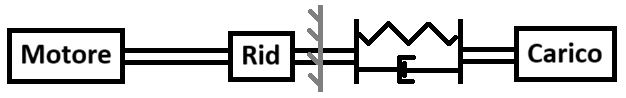
\includegraphics[width=0.5\textwidth]{Immagini/schema_antirisonanza.png}
    \caption{Schema equivalente per verifica su antirisonanza}
\end{figure}

\paragrafo{Relazione poli-zeri Gvm:}
Ricordando rapporto di inerzia \(\rho = \frac{\tau_R^2 J_c}{J_m} > 0\), in \(G_{vm}(s)\) esiste una relazione tra pulsazione del polo e pulsazione dello zero e per smorzamento del polo e smorzamento dello zero:
\[
\begin{cases}
    \omega_p = \omega_z \sqrt{1+\rho} \\
    \xi_p = \xi_z \sqrt{1+\rho} \\
    \omega_z < \omega_p \\
    \xi_z < \xi_p
\end{cases}
\]

\begin{figure}[h]
    \centering
    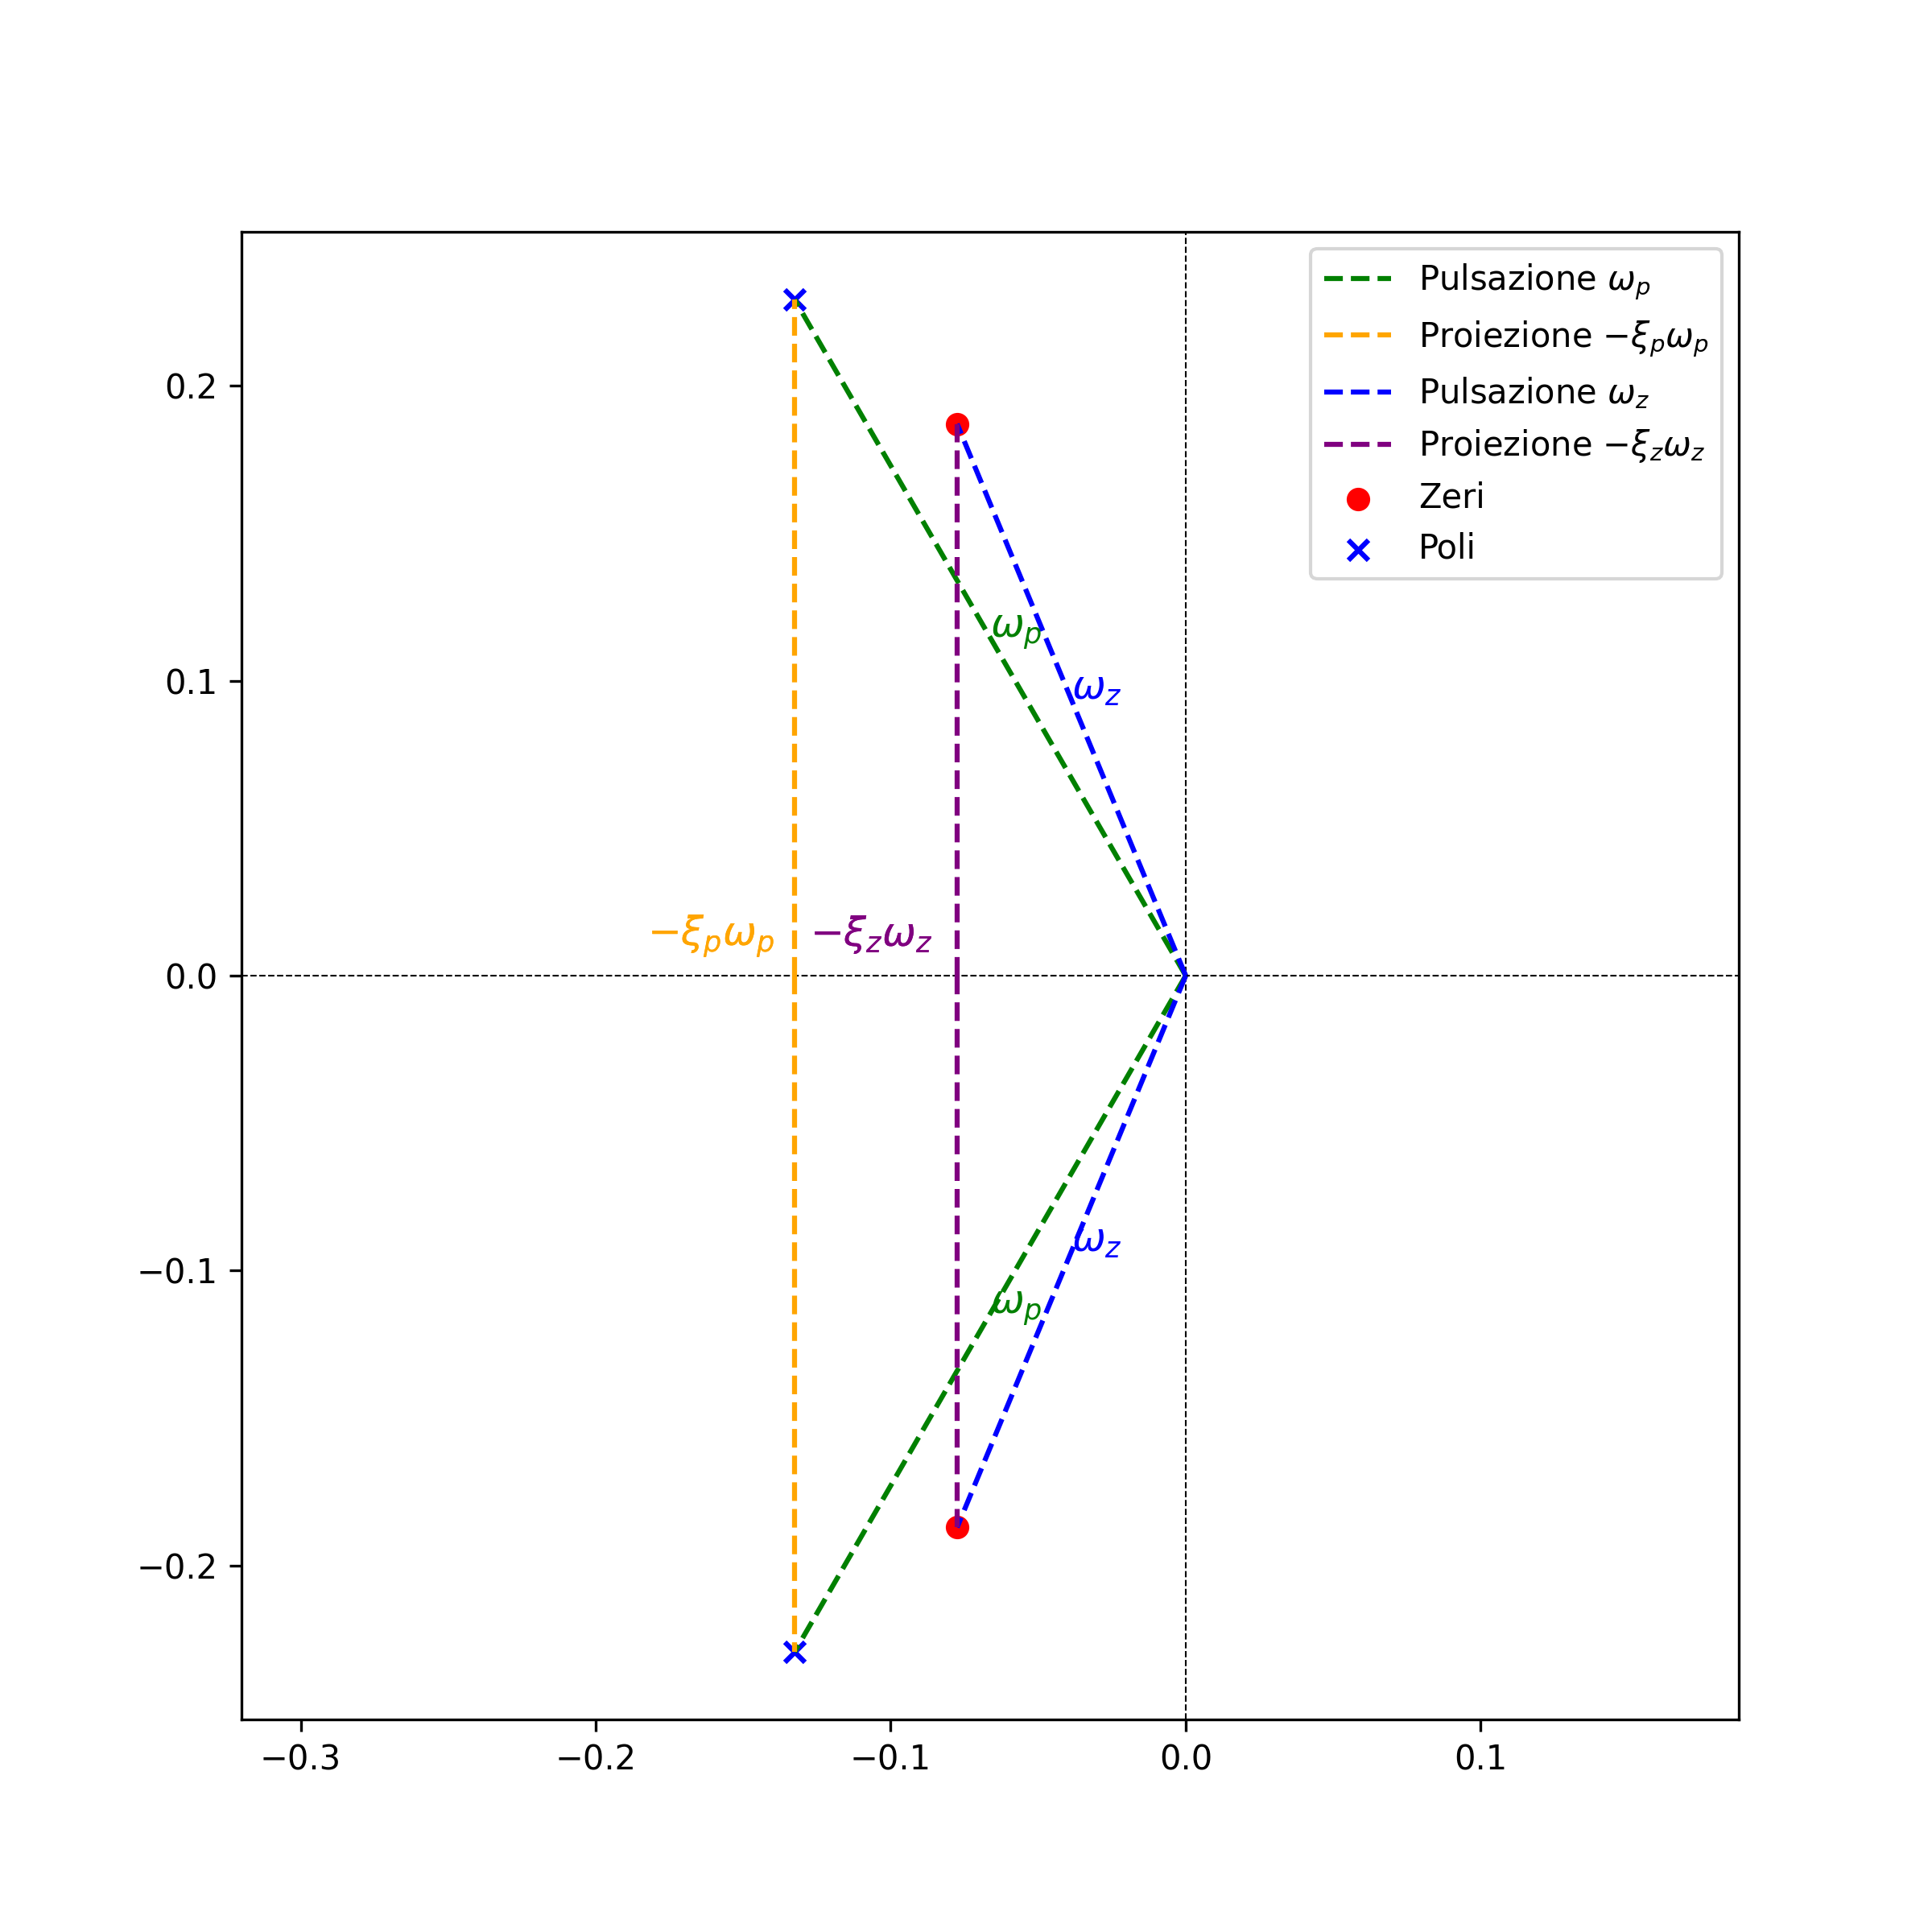
\includegraphics[width=0.5\textwidth]{Immagini/poli_zeri_Gvm.png}
    \caption{Rappresentazione su piano complesso di poli e zeri di \(G_{vm}\)}
\end{figure}

\sezione{Architetture di controllo}
Ci sono diverse tipologie di controllo in base alla grandezza misurata (o stimata) e grandezza attuata e se sono riferite entrambe allo stesso sitema (entrambe motore oppure una motore l'altra carico) o all'utilizzo di controllo SISO o MIMO.

\paragrafo{Controllo Co-Locato:}
Con controllo co-locato si intende un controllo in cui misura e grandezza attuata sono al motore; il carico si trova all'esterno del loop ed è in catena aperta.

\import{Immagini}{controllo_co_locato}

\paragrafo{Controllo non Co-Locato:}
Con controllo non co-locato si intende un controllo in cui misura e grandezza attuata sono differenti, in particolare la misura è effettuata al carico mentre la grandezza attuata è al motore; il carico si trova all'interno del loop.

\import{Immagini}{controllo_non_co_locato}

\paragrafo{Controllo di stato:}
Nel controllo di stato, lavorando in MIMO, permette di scegliere entrambe le grandezza di misura, risultando in un controllo migliore. Tuttavia nell'industria sono solitamente difficilmente praticabili. 

\sottosezione{Controllo Co-Locato vs non Co-Locato}
Per valutare quale controllo utilizzare vado a studiare intanto il controllo Co-Locato e in particolare l'inertanza (per semplicità di analisi) \(sG_{vm}(s)\) e la mobilità \(G_{vm}(s)\). Per il tracciamento si consiglia di studiare gli asintoti e quindi tracciare la funzione di trasferimento collegandoli.
Si notano in particolare \(m_\phi > 90^\circ\) e, non arrivando mai a \(-180^\circ\), vale anche \(m_a = \infty\). Questo è un ottimo segnale in termini di stabilità del sistema.\footnote{In fase, variazione tra \(-360^\circ\rightarrow -180^\circ\) equivale alla variazione \(0^\circ\rightarrow 180^\circ\) vista in aula}

\begin{figure}[h]
    \centering
    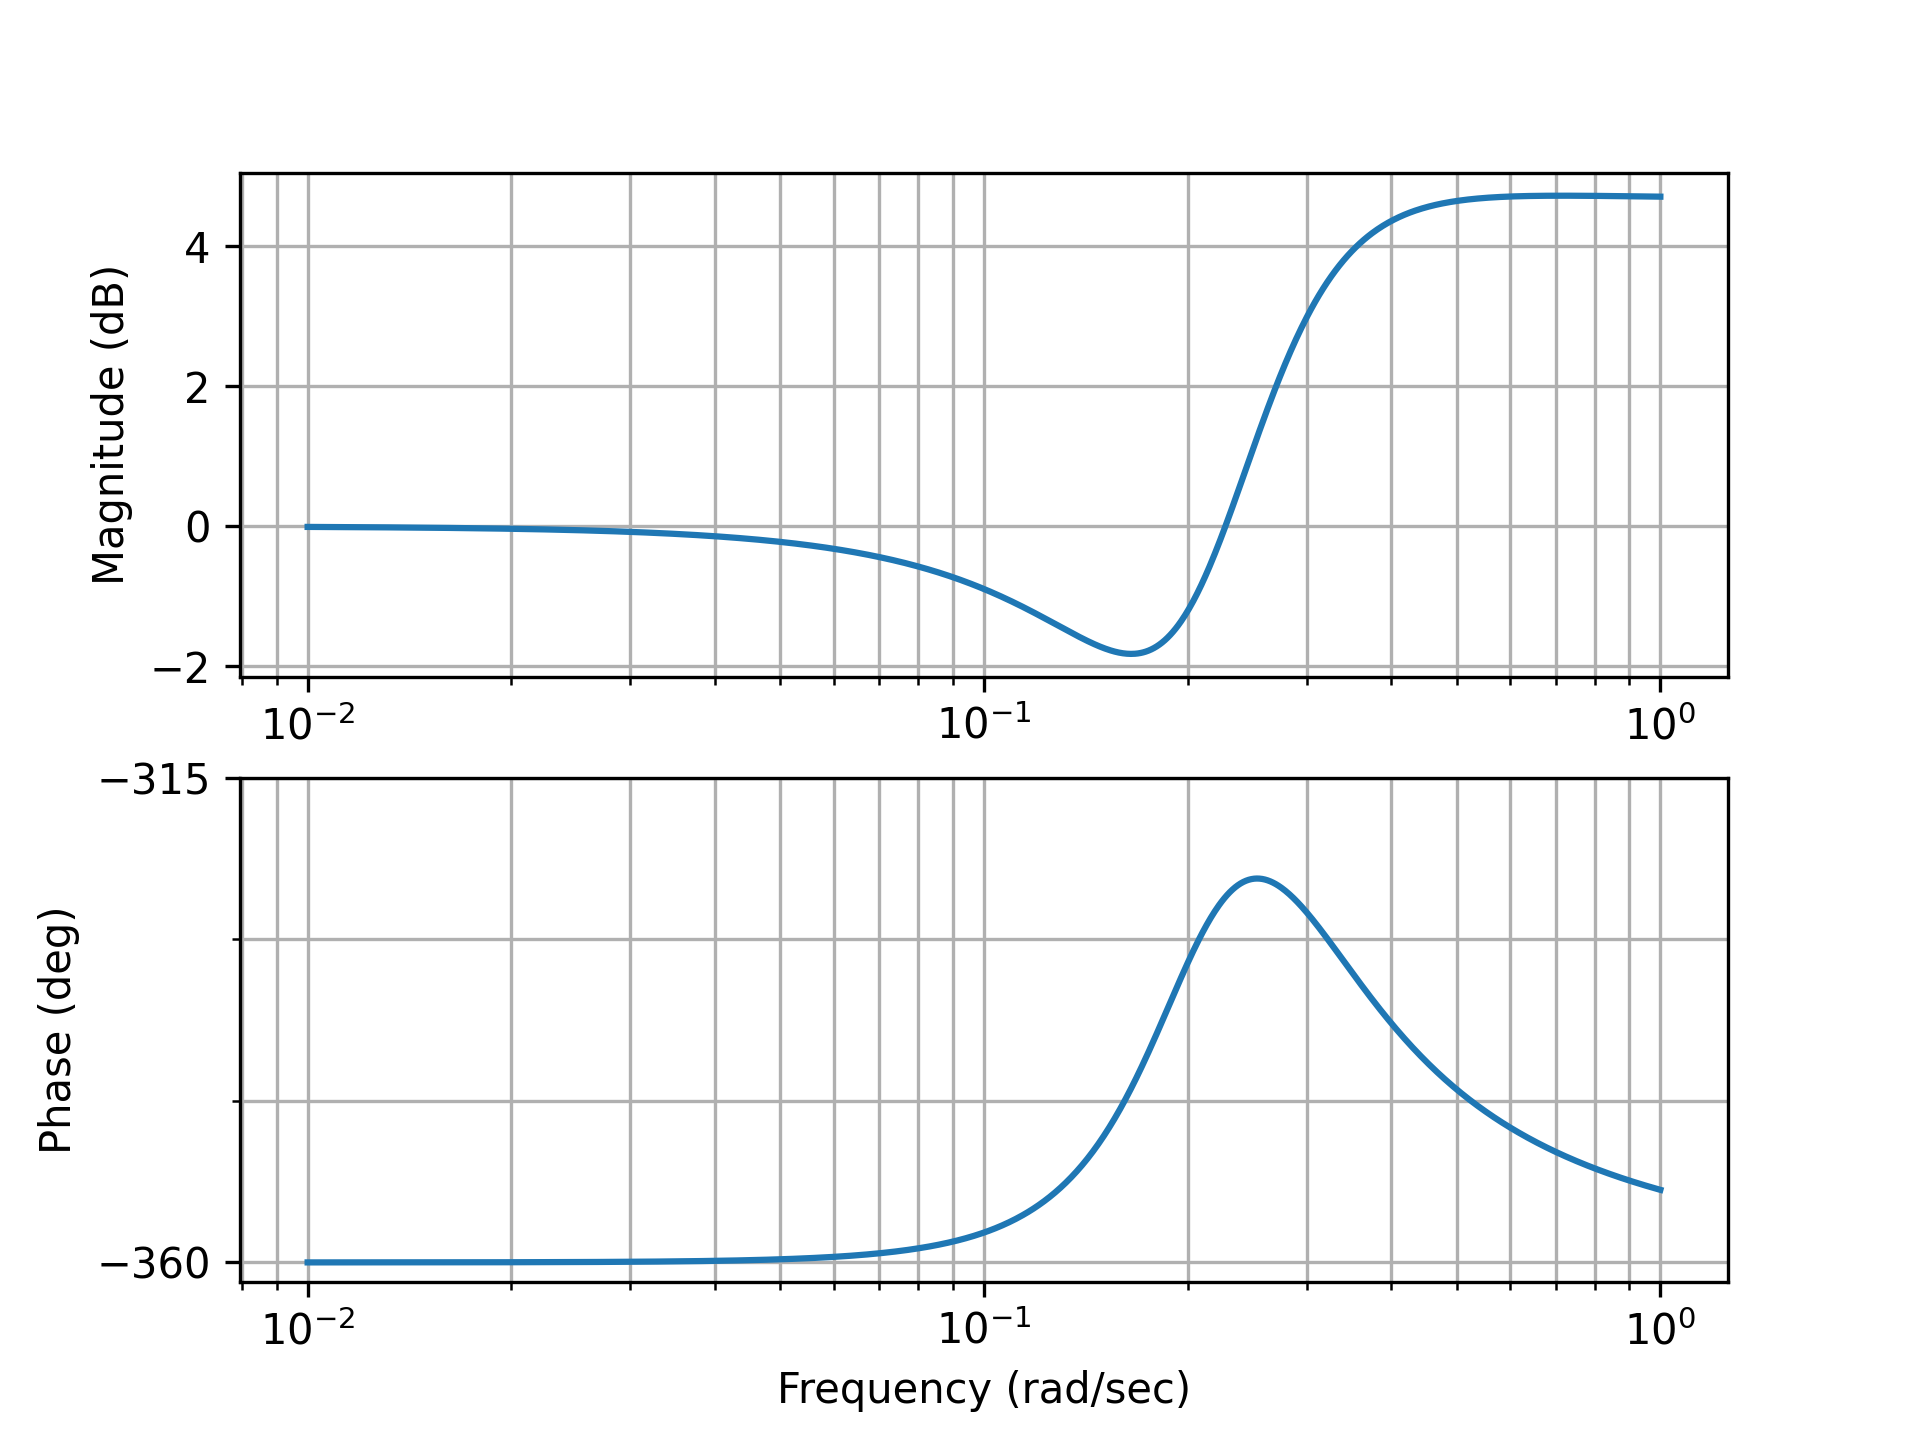
\includegraphics[width=0.45\textwidth]{Immagini/Inertanza_gvm.png}
    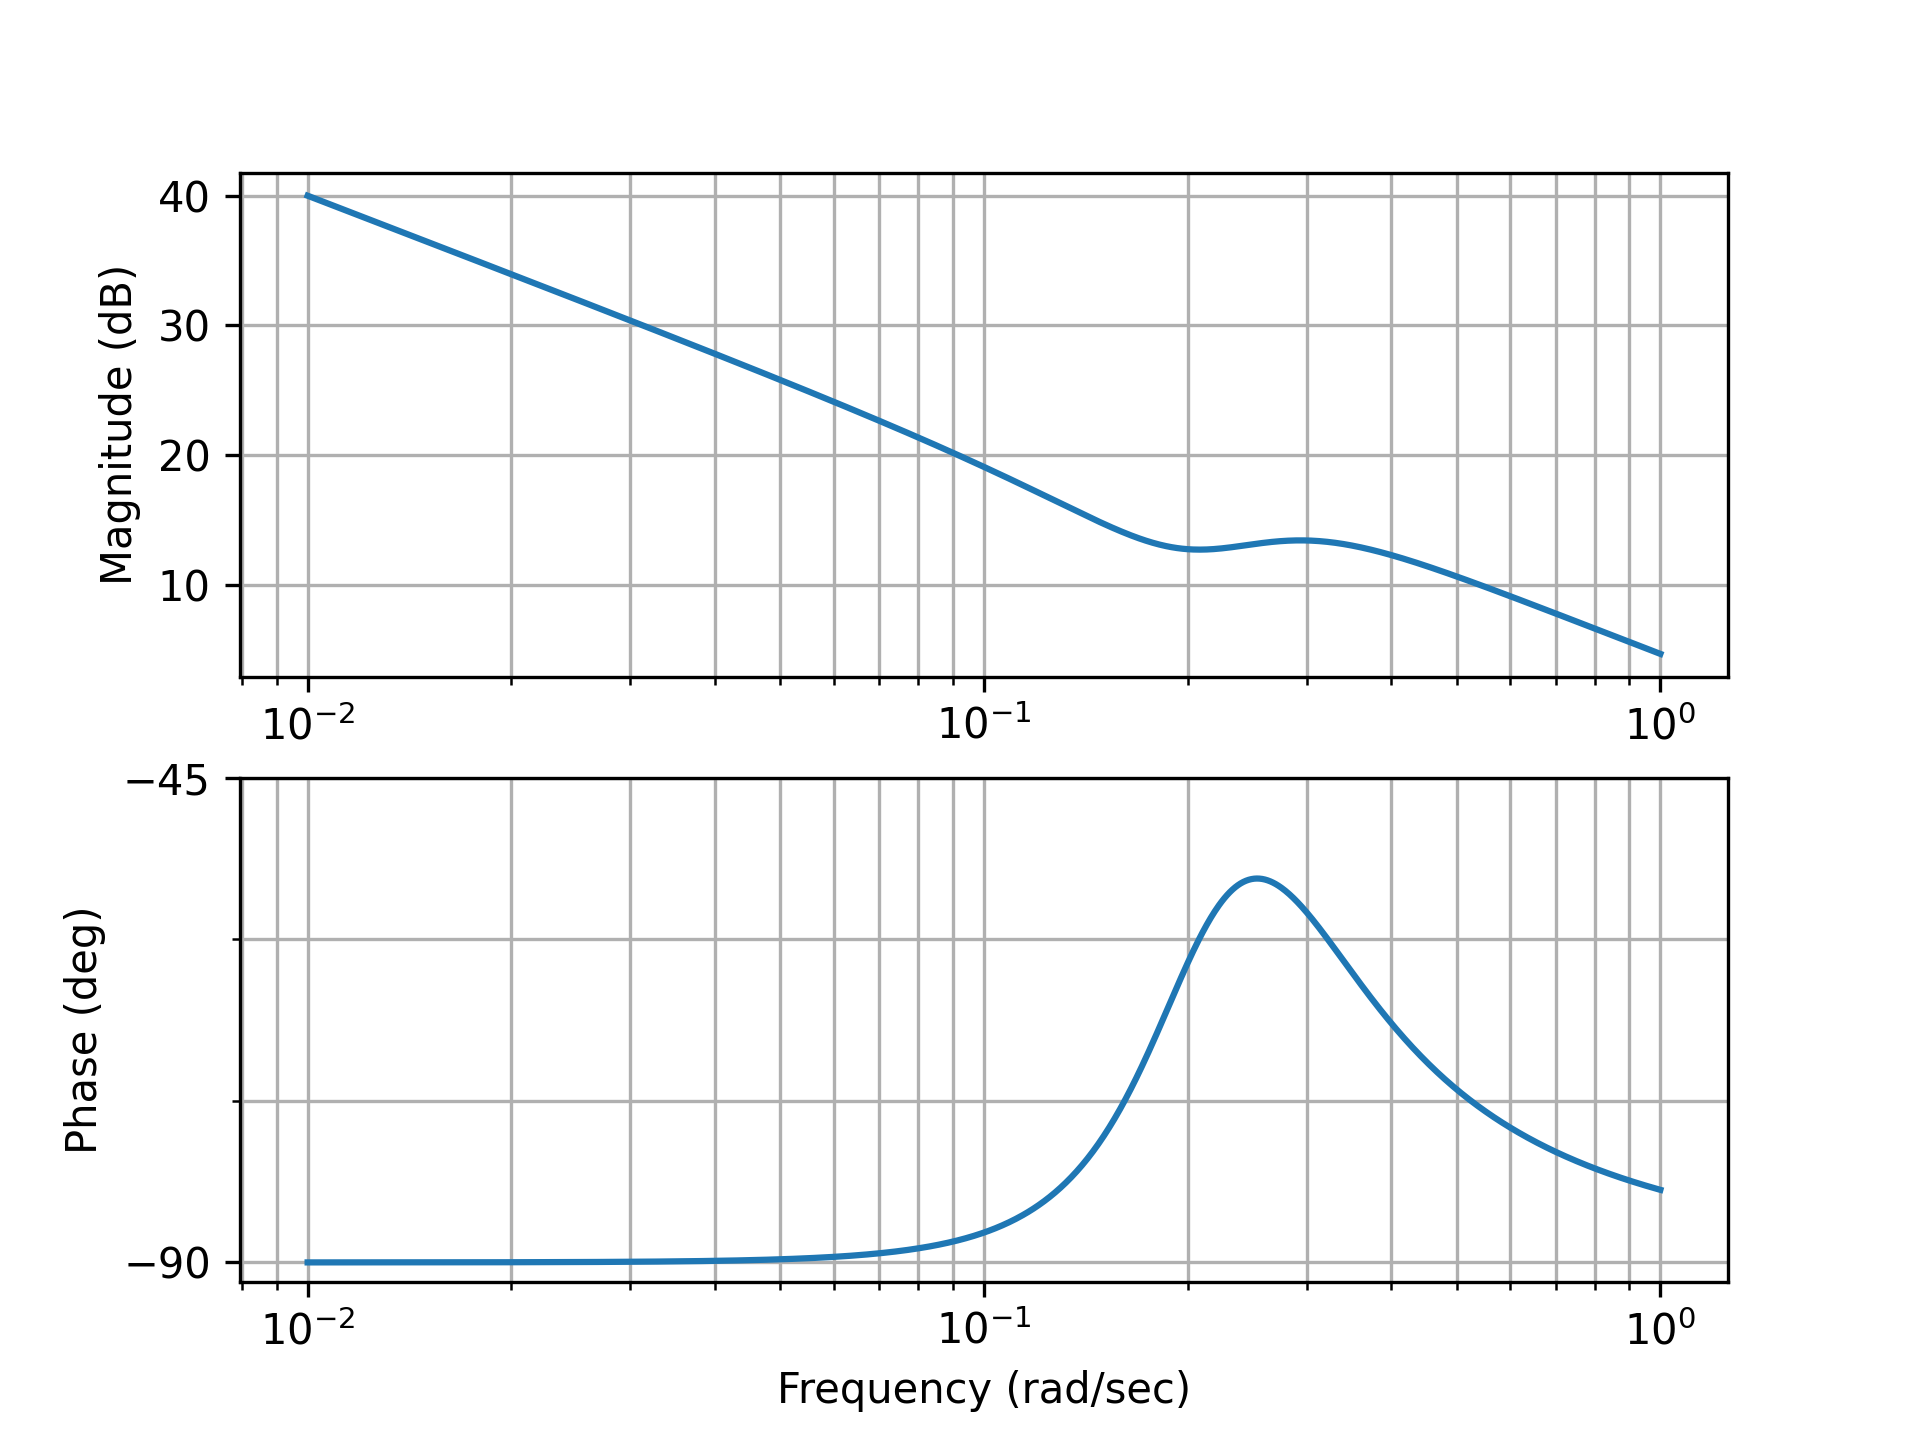
\includegraphics[width=0.45\textwidth]{Immagini/mobilita_gvm.png}
    \caption{Inertanza \(sG_{vm}\) sx e mobilità \(G_{vm}\)}
\end{figure}

\paragrafo{Controllo non Co-Locato:}
Per quanto riguarda il controllo non Co-Locato, facendo lo stesso ci si accorge di come la mobilità, complessivamente sia un sistema con polo del secondo ordine, inoltre il polo agisce prima dello zero, quindi in un certo tratto la fase potrebbe andare al di sotto dei \(-180^\circ\). Come risulta più chiaro dal grafico, questo aspetto ha conseguenze sulla stabilità del sistema: \textbf{Non si può fare un controllo non co-locato in velocità.}

\begin{figure}[h]
    \centering
    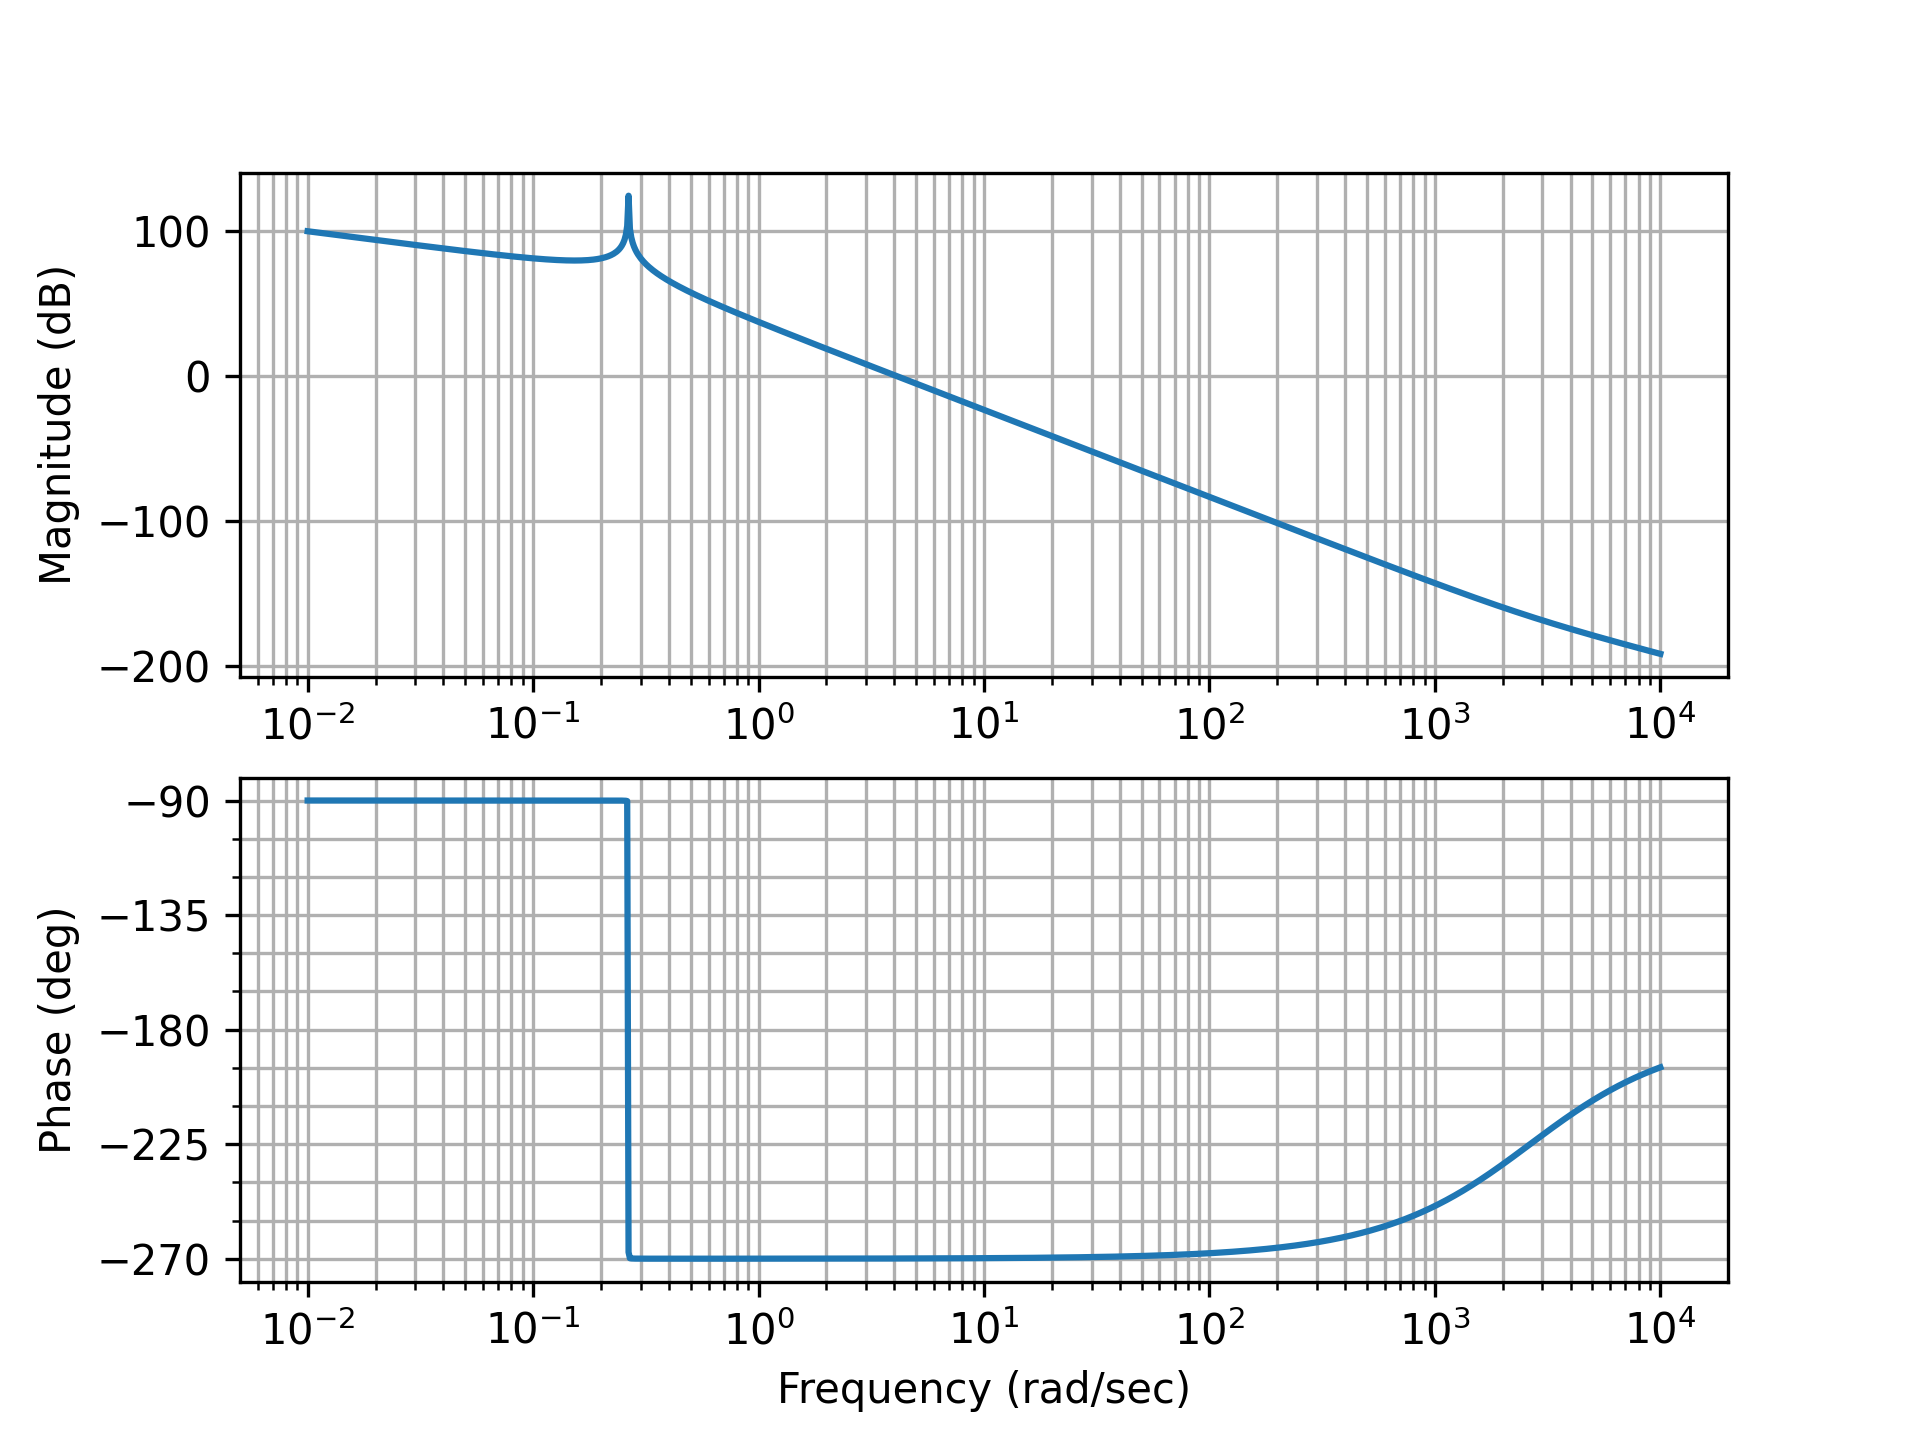
\includegraphics[width=0.45\textwidth]{Immagini/mobilita_gvc.png}
    \caption{Mobilità \(G_{vc}\)}
\end{figure}

\paragrafo{Luogo delle radici:}
Valutazioni simili possono essere fatte utilizzando il luogo delle radici\footnote{Vedi \ref{rlocus} per le regole di tracciamento, noi lavoreremo in modo qualitativo, quindi senza valutare esattamente gli asintoti, gli angoli di uscita o il passaggio per l'asse immaginario.}.

\begin{figure}[h]
    \centering
    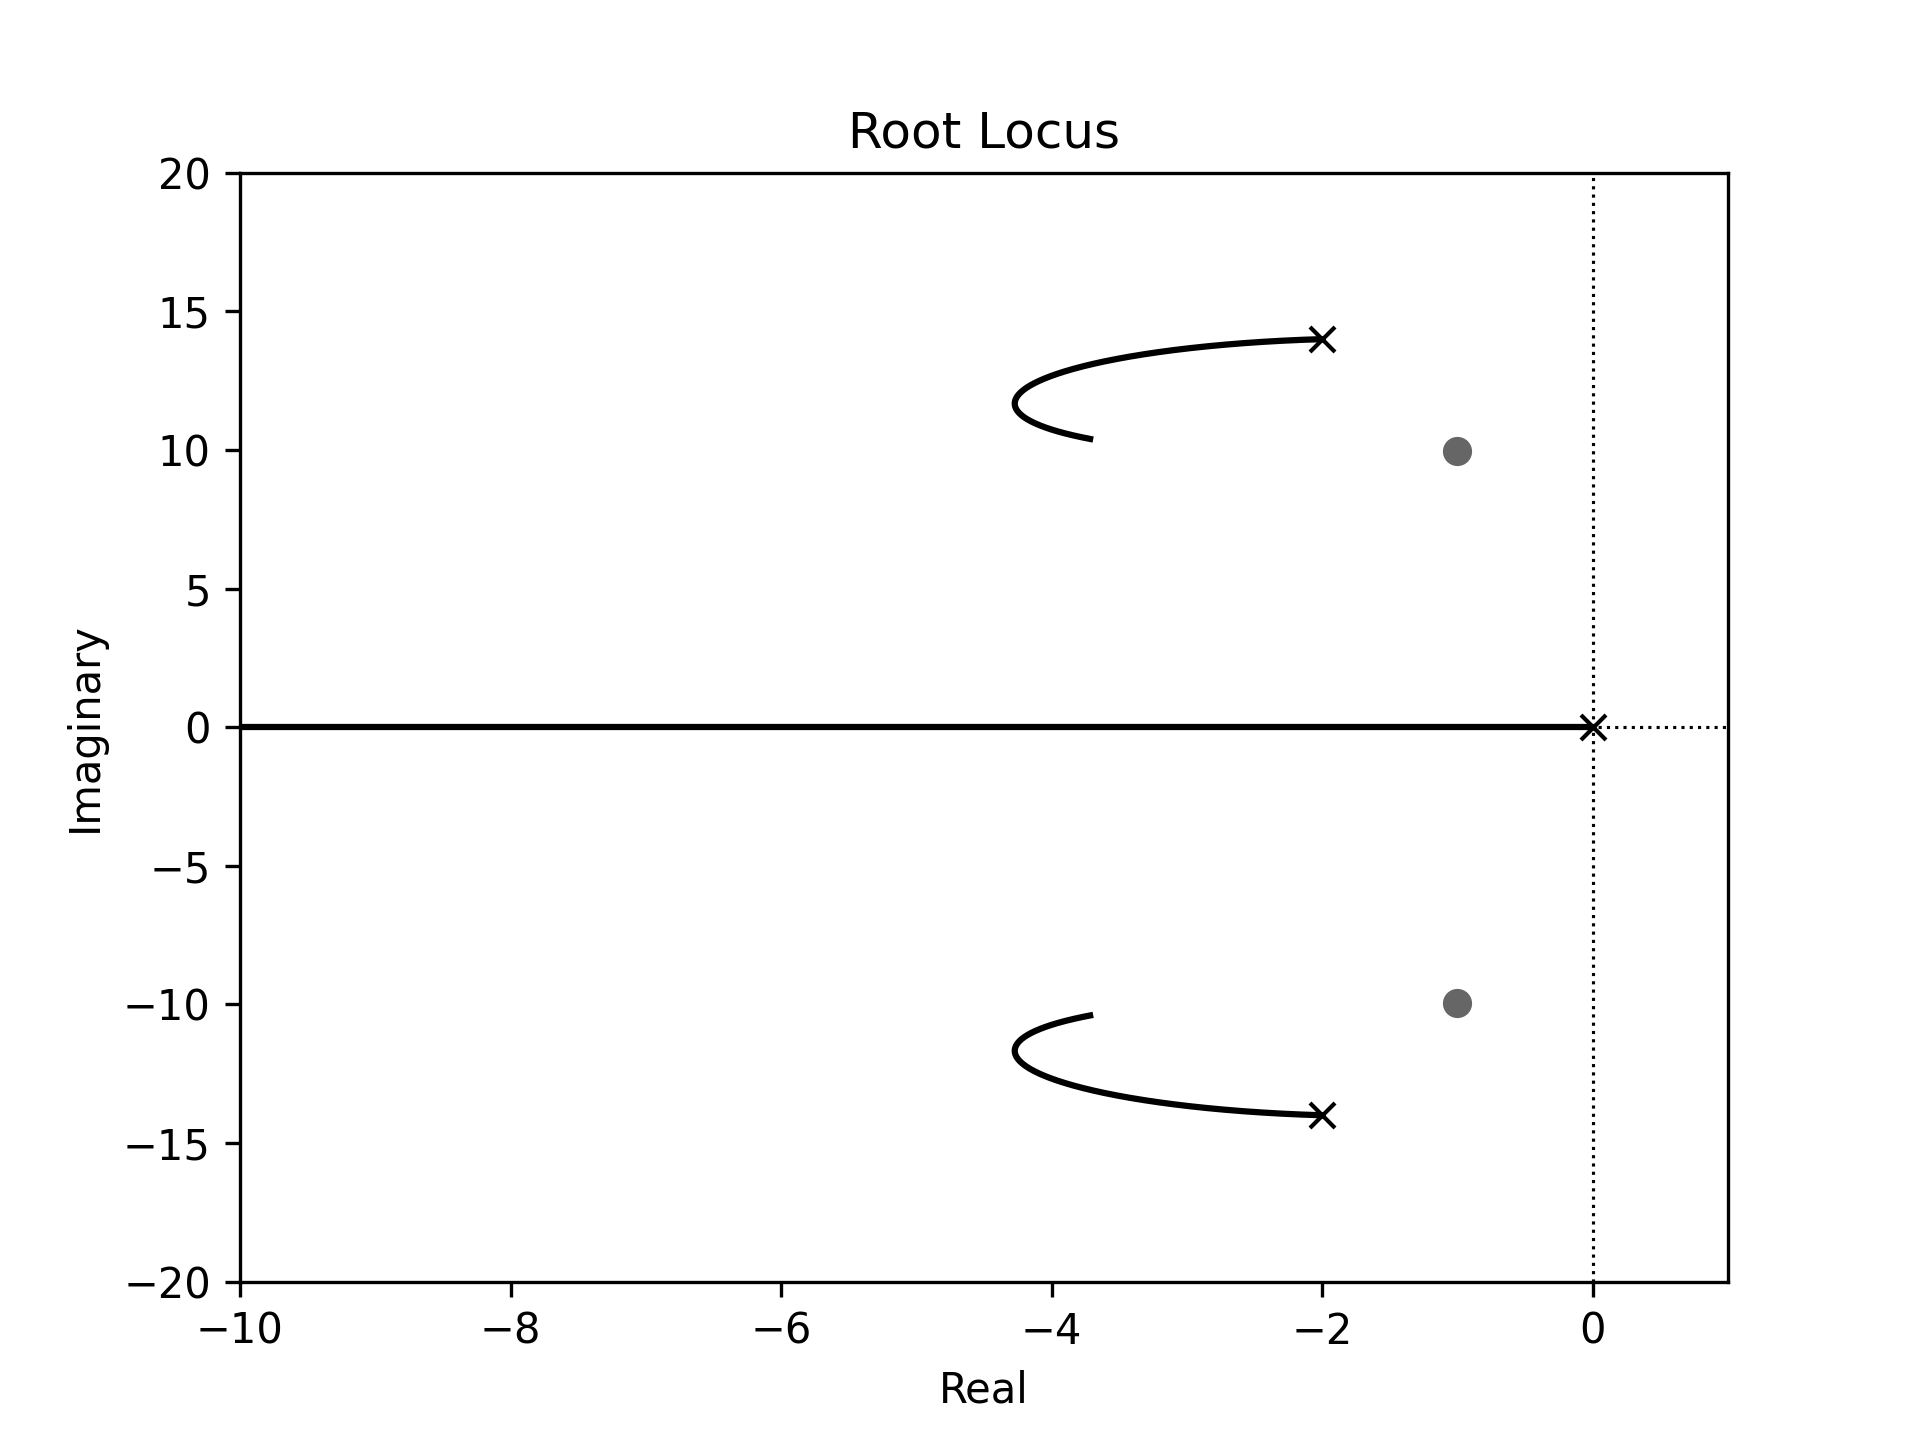
\includegraphics[width=0.45\textwidth]{Immagini/controllo_v_colocato.png}
    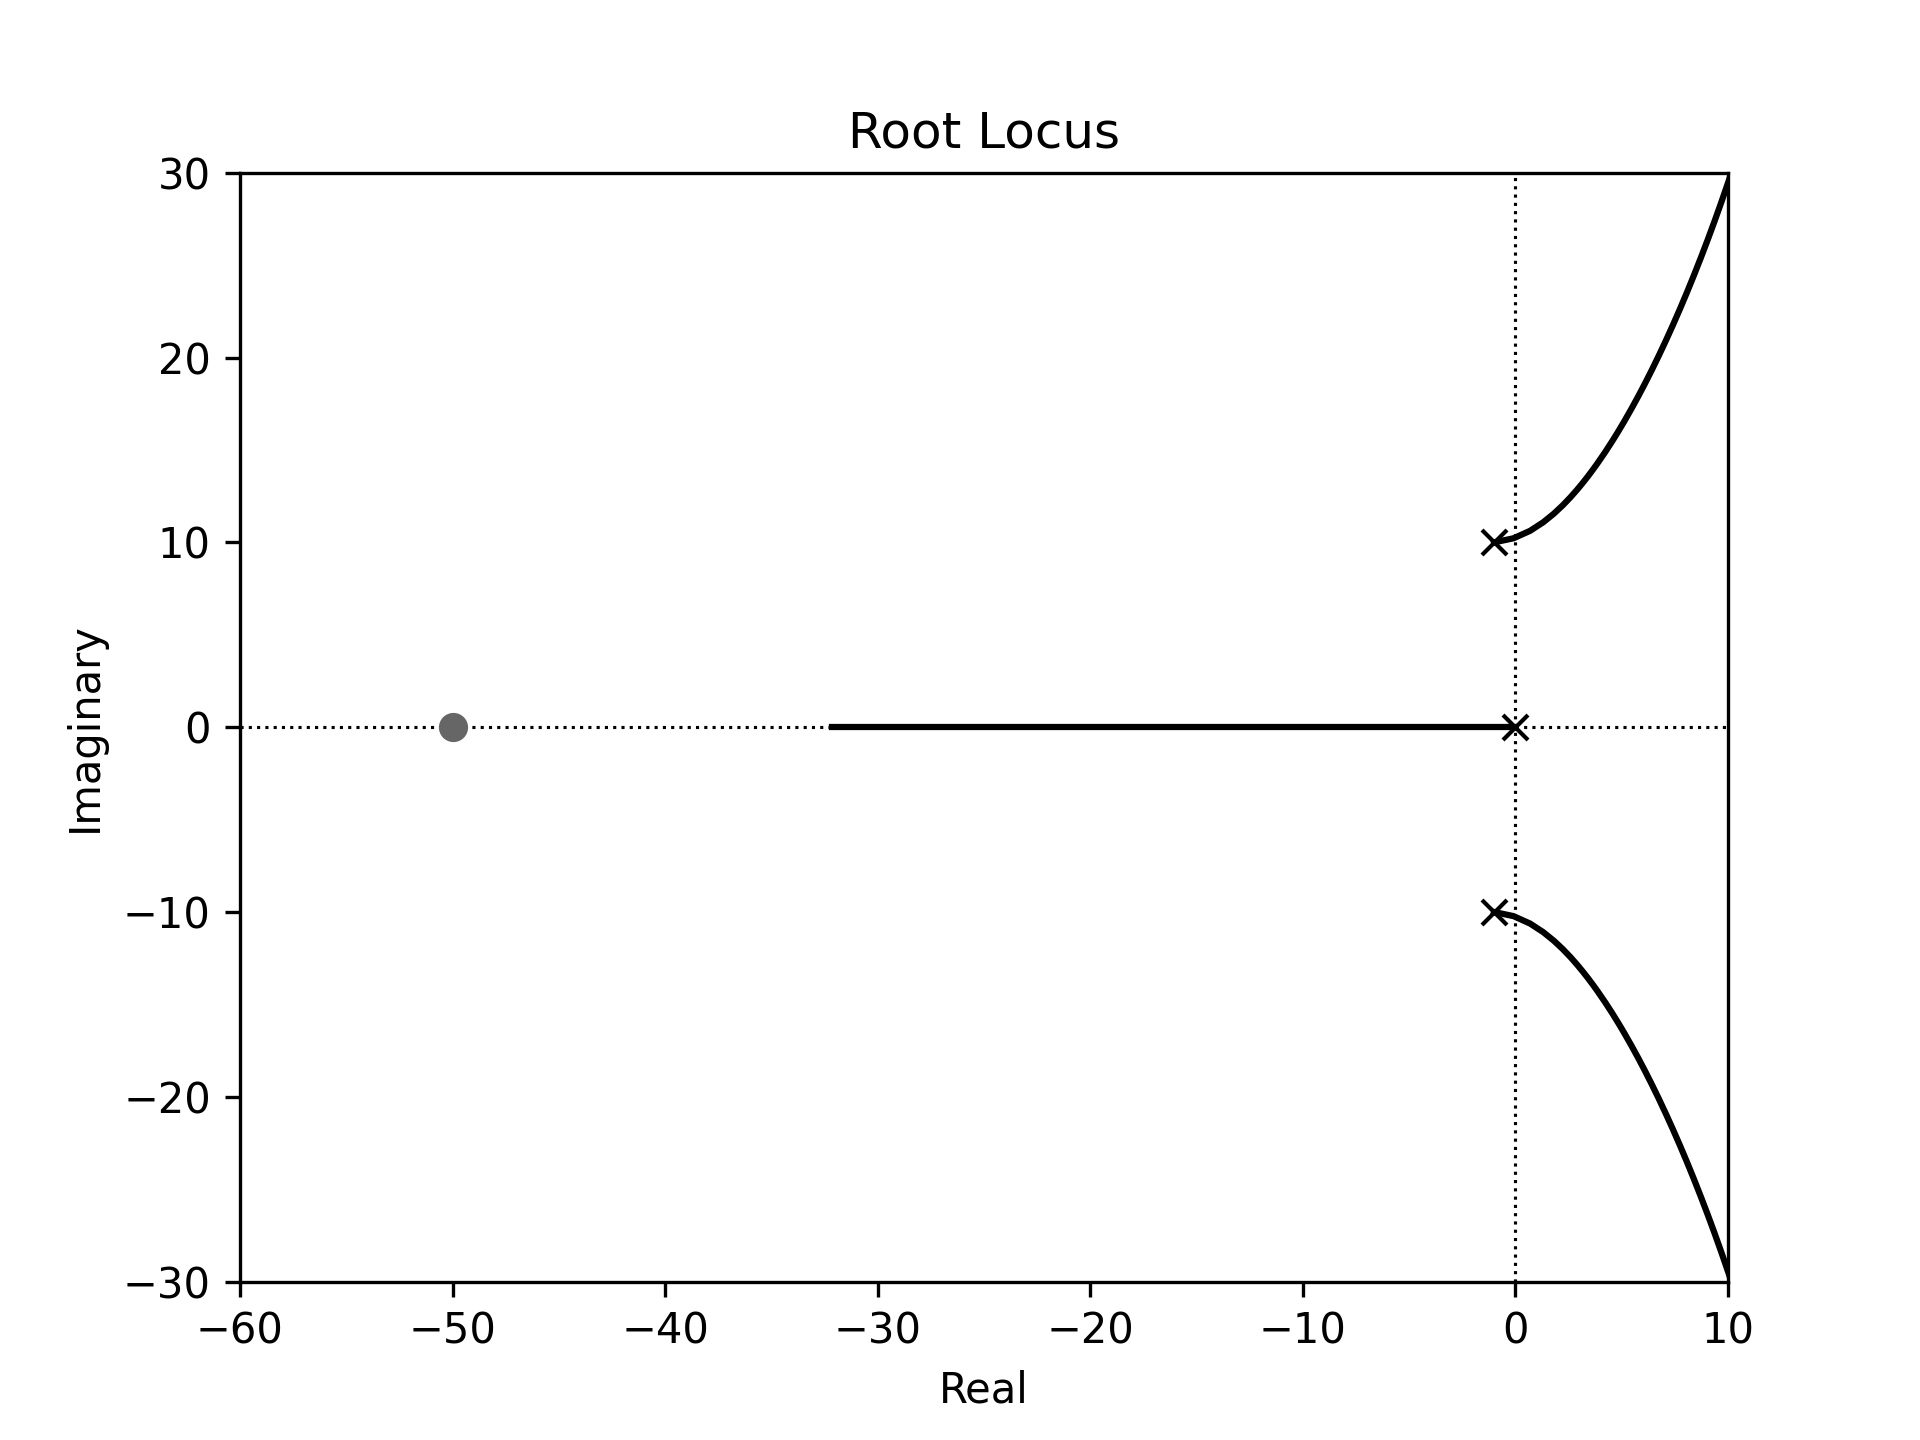
\includegraphics[width=0.45\textwidth]{Immagini/controllo_v_non_colocato.png}
    \caption{Controlli di velocità: Co-Locato sx; Non Co-Locato dx}
\end{figure}

\sottosezione{Trasmissibilità}
A completamento dell'analisi, si può studiare anche la trasmissibilità \(T(s) = \tau \frac{1+\frac{2\xi_z}{\omega_z}s}{1+\frac{2\xi_z}{\omega_z}s + \frac{s^2}{\omega_z^2}}\). Da notare come ad alta frequenza (come visto in Meccanica delle Vibrazioni) vi sia la zona di non trasmissione del moto, con modulo fortemente attenuato e ritardo. Il moto relativo di motore e carico è "grande".

\begin{figure}[h]
    \centering
    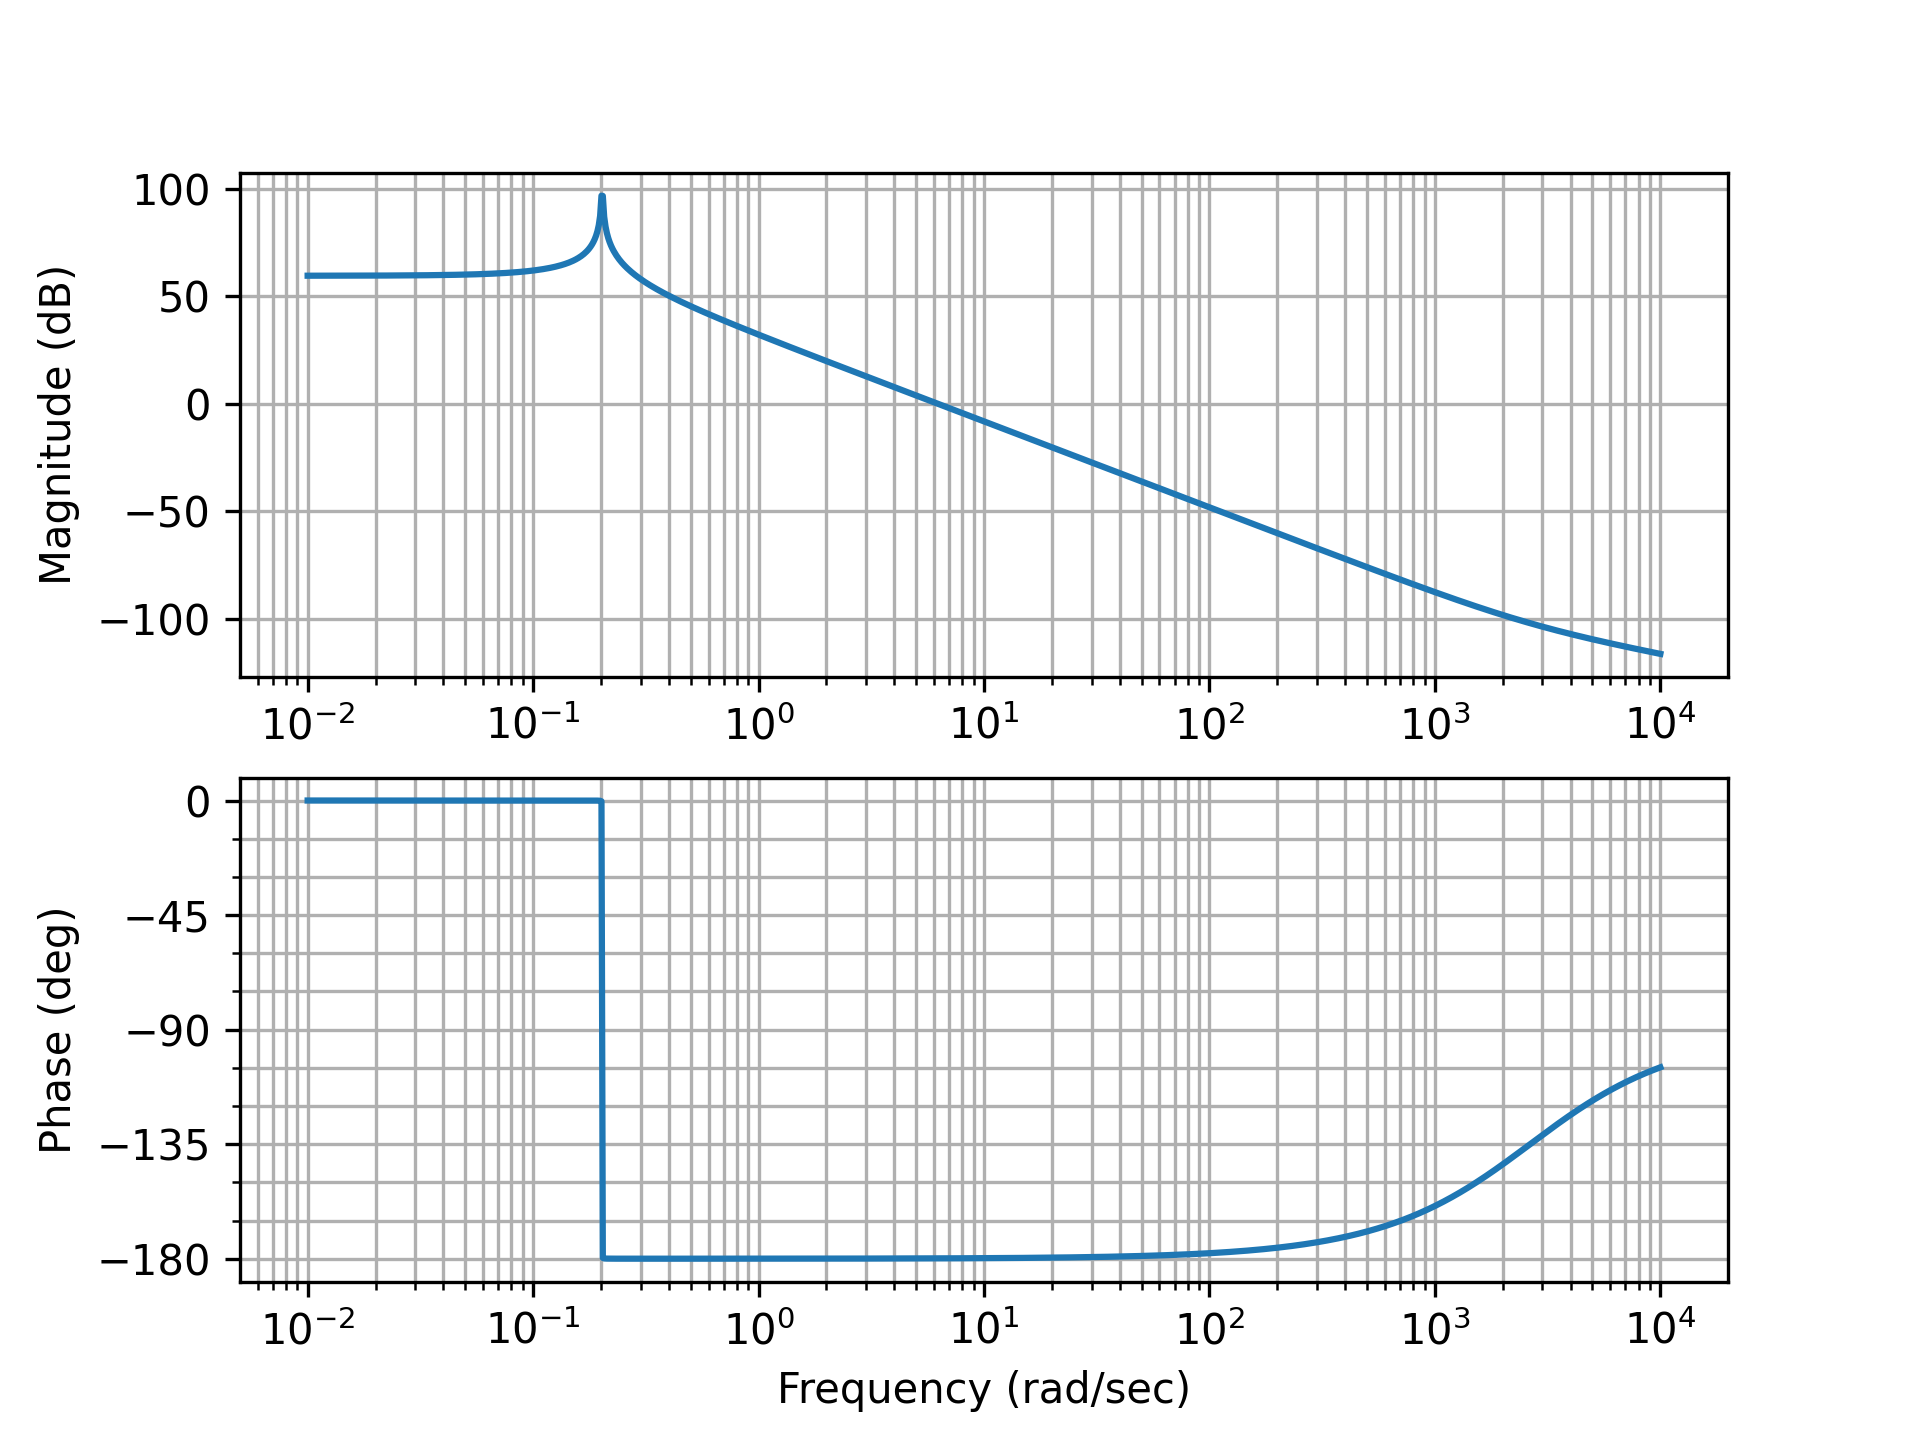
\includegraphics[width=0.45\textwidth]{Immagini/trasmissibilita.png}
    \caption{Trasmissibilità \(T(s)\)}
\end{figure}

\sottosezione{Attrito}
L'attrito ha implicazioni in tutto il sistema, volessi fare un'analisi rigorosa dovrei ricalcolare gli smorzamenti e le pulsazioni. Per un analisi approssimata invece è sufficiente considerare come l'attrito vada ad agire principalmente sul sistema rigido, quindi soprattutto per basse frequenze, si ottiene quindi il modello: \(G_{vm}(s) \simeq \frac{1}{sJ+f} \frac{\frac{s^2}{\omega_z^2} + \frac{2\xi_z}{\omega_z} s + 1}{\frac{s^2}{\omega_p^2} + \frac{2\xi_p}{\omega_p} s + 1}\). 

A differenza del precedente, al posto di avere un integrale in ingresso c'è un filtro passa basso, che in alta frequenza si comporta esattamente come un integrale.

In senso fisico, l'attrito è legato al moto assoluto (più rilevante in bassa frequenza), mentre l'attrito viscoso è maggiormente legato al moto relativo (più rilevante in alta frequenza).

\sezione{Controllo Co-Locato di Velocità}
Valutato come il controllo da utilizzare in velocità sia quello Co-Locato, considero due casi:
\[
\frac{\omega_p}{\omega_z} = \frac{\xi_p}{\xi_z} = \sqrt{1+\rho} \ \rightarrow \
\begin{cases}
    \rho \rightarrow 0 \text{ , allora } \omega_p\simeq \omega_z, \xi_p\simeq \xi_z \text{ cancellazione fisica polo-zero} \\
    \rho >> 0 \text{ , allora } \omega_p >> \omega_z, \xi_p >> \xi_z \text{ poli zeri ben distinti}
\end{cases}
\]


Dal luogo delle radici è possibile verificare come, col variare di \(K_{pv}\), varino: 
\begin{itemize}
    \item la lunghezza del vettore che collega origine e punti del luogo, che corrisponde alla variazione di pulsazione dei poli del sistema a catena chiusa \(W_v\)
    \item l'angolo del vettore, che corrisponde alla variazione di fattore di smorzamento del polo di \(W_v\)
    \item la proiezione del vettore sull'ascissa, che corrisponde a \(\abs{\mathbb{R}(W_v)}\)
\end{itemize}

\paragrafo{Significato fisico:}
\(\rho \simeq 1\) significa motore e carico di massa paragonabili. Il motore percepisce oscillazioni del carico, può quindi attivarsi per cercare di limitarle.
\(\rho \rightarrow 0\) significa motore di massa tanto maggiore a quella del carico. Il controllo viene visto come semplificato perché qualsiasi problematica di carico non viene percepita dal motore. Soluzione per questo caso è quella di utilizzare un controllo in controllo di stato (se possibile) oppure scegliere una legge di moto dolce standard o ad hoc (in particolare leggi di moto dolci ad hoc per \(\rho \rightarrow 0\) si vedranno in laboratorio).

\begin{figure}[h]
    \centering
    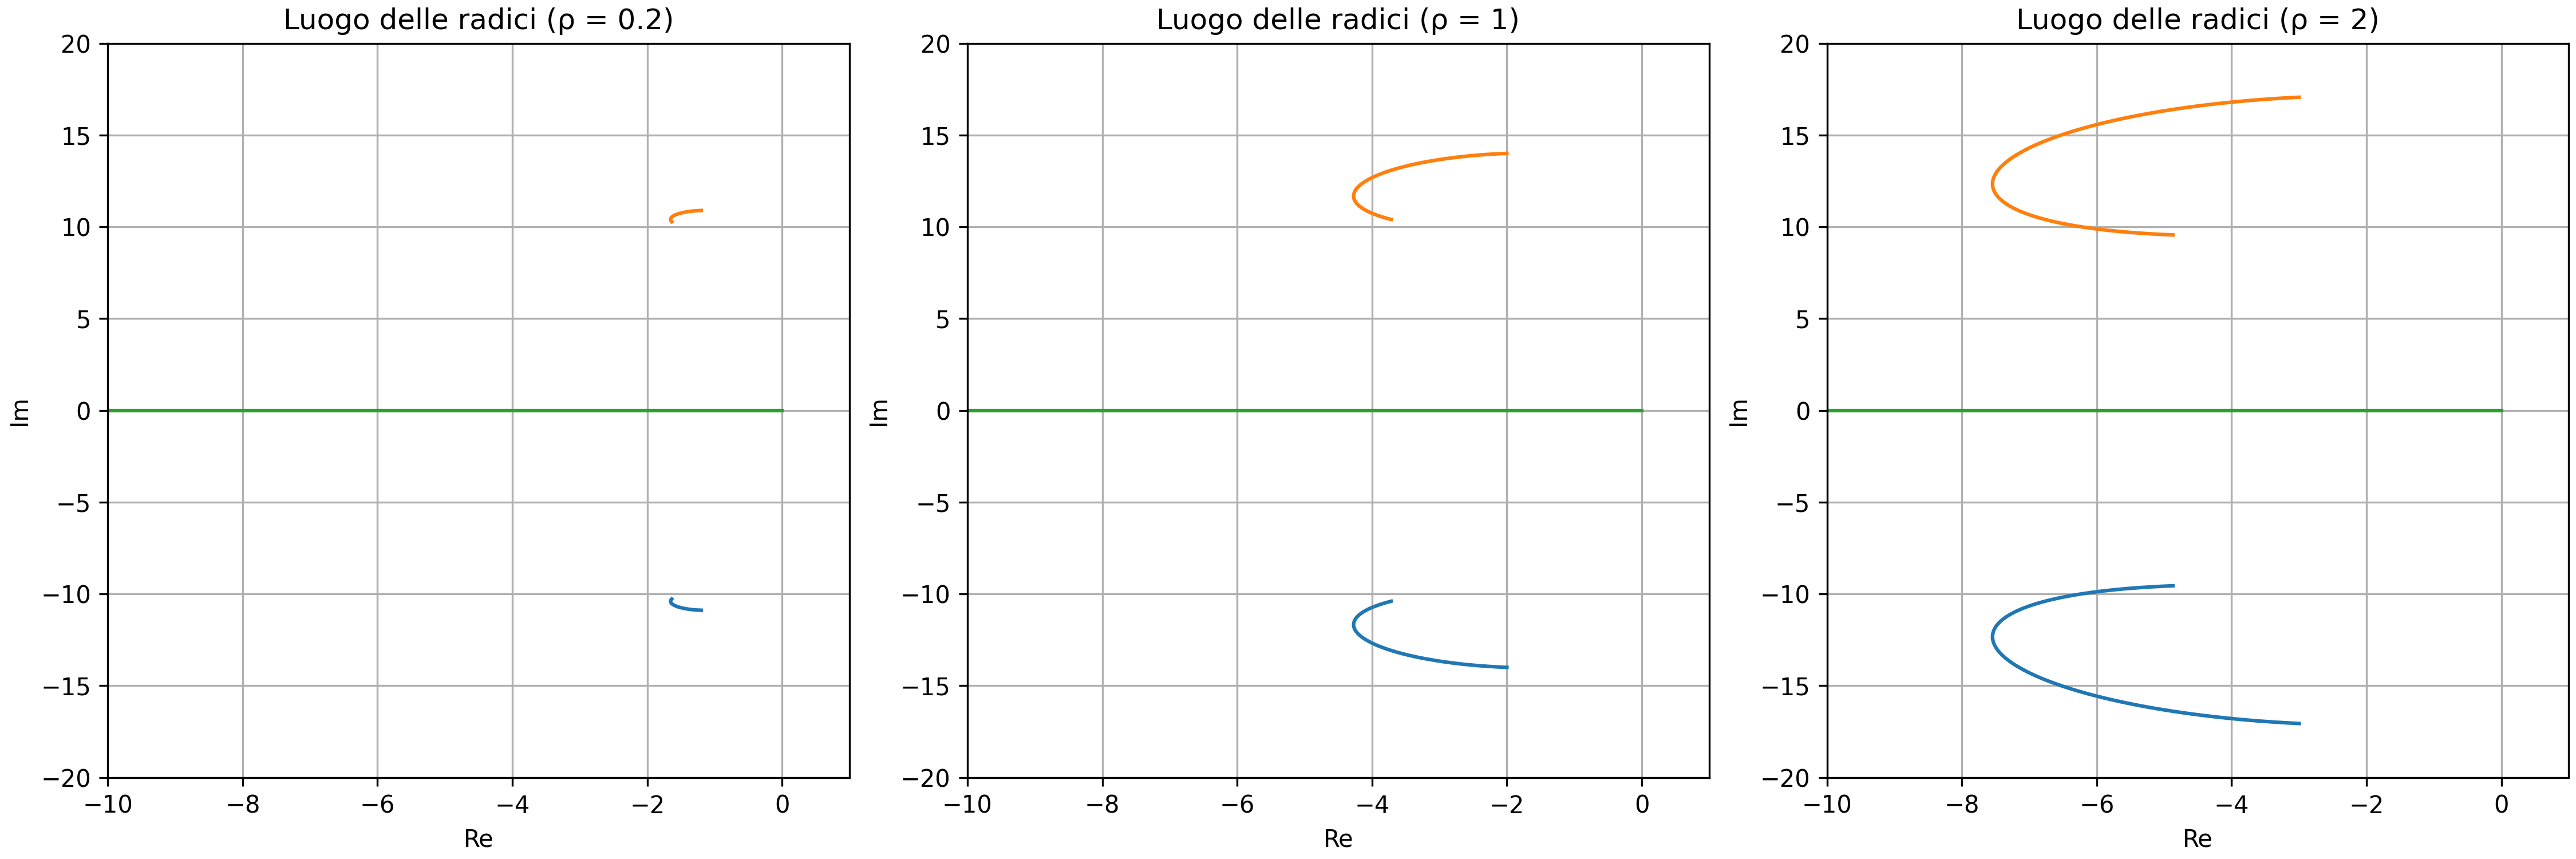
\includegraphics[width=0.8\textwidth]{Immagini/controllo_v_colocato_subplot_rho.png}
    \caption{Controllo Co-Locato per vari \(\rho\)}
\end{figure}

\paragrafo{Relazione smorzamento massimo di Wv e rho:}
Sussiste una relazione tra il massimo smorzamento dei poli di \(W_v\) e \(\rho\): \(\xi_{max} = \xi_p + \frac{\sqrt{1+\rho}}{2} - 1\). Questa relazione (non da sapere a memoria) evidenzia come lo smorzamento massimo dei poli di \(W_v\) sia maggiore di quello dei poli a catena aperta, ed è legato a quanto visto per il luogo delle radici in cui è evidente la dipendenza tra \(\rho\) e \(\alpha\).

\sottosezione{Rapporto di inerzia nullo}
Per \(\rho \rightarrow 0\) il controllo di motore è equivalente al controllo di un asse rigido, avente \(\omega_{bv}\) elevata. La banda elevata può portare il motore ad eccitare il carico, se comandato con legge di moto non dolce. 

Considero l'errore di posizione al carico: \(e_c(t) = \theta_c^{des}(t) - \theta_c^{mis}(t)\) considerando \(\tau=1\), solo per semplificare il ragionamento, e \(\theta_c^{mis} = \theta_c\) ossia che il motore venga controllato bene (ipotesi realistica, considerando che sto lavorando con un equivalente asse rigido) \(e_c(t) = \theta_M^{des}(t) - \theta_c(t)\), passando in Laplace si ottiene \(E(s) = \theta_M (s) - \theta_c(s) = \theta_M(s) (1 - T(s)) = \theta_M(s) \frac{\frac{s^2}{\omega_z^2}}{\frac{s^2}{\omega_z^2} + \frac{2\xi_z}{\omega_z}s + 1}\), da cui si ottiene la formulazione:
\[
E(s) = \frac{A_M(s)}{\omega_z^2} \frac{1}{\frac{s^2}{\omega_z^2} + \frac{2\xi_z}{\omega_z}s + 1}
\]

In cui viene evidenziata la relazione tra errore in posizione motore-carico e accelerazione del motore. Questo ha conseguenze sulla scelta della legge di moto perché avere accelerazione maggiore (a parità di altro), è associato ad accelerazioni maggiore. Inoltre viene evidenziato l'effetto della pulsazione dello zero \(\omega_z\) che va ad abbattere l'errore di posizione.

\begin{figure}[h]
    \centering
    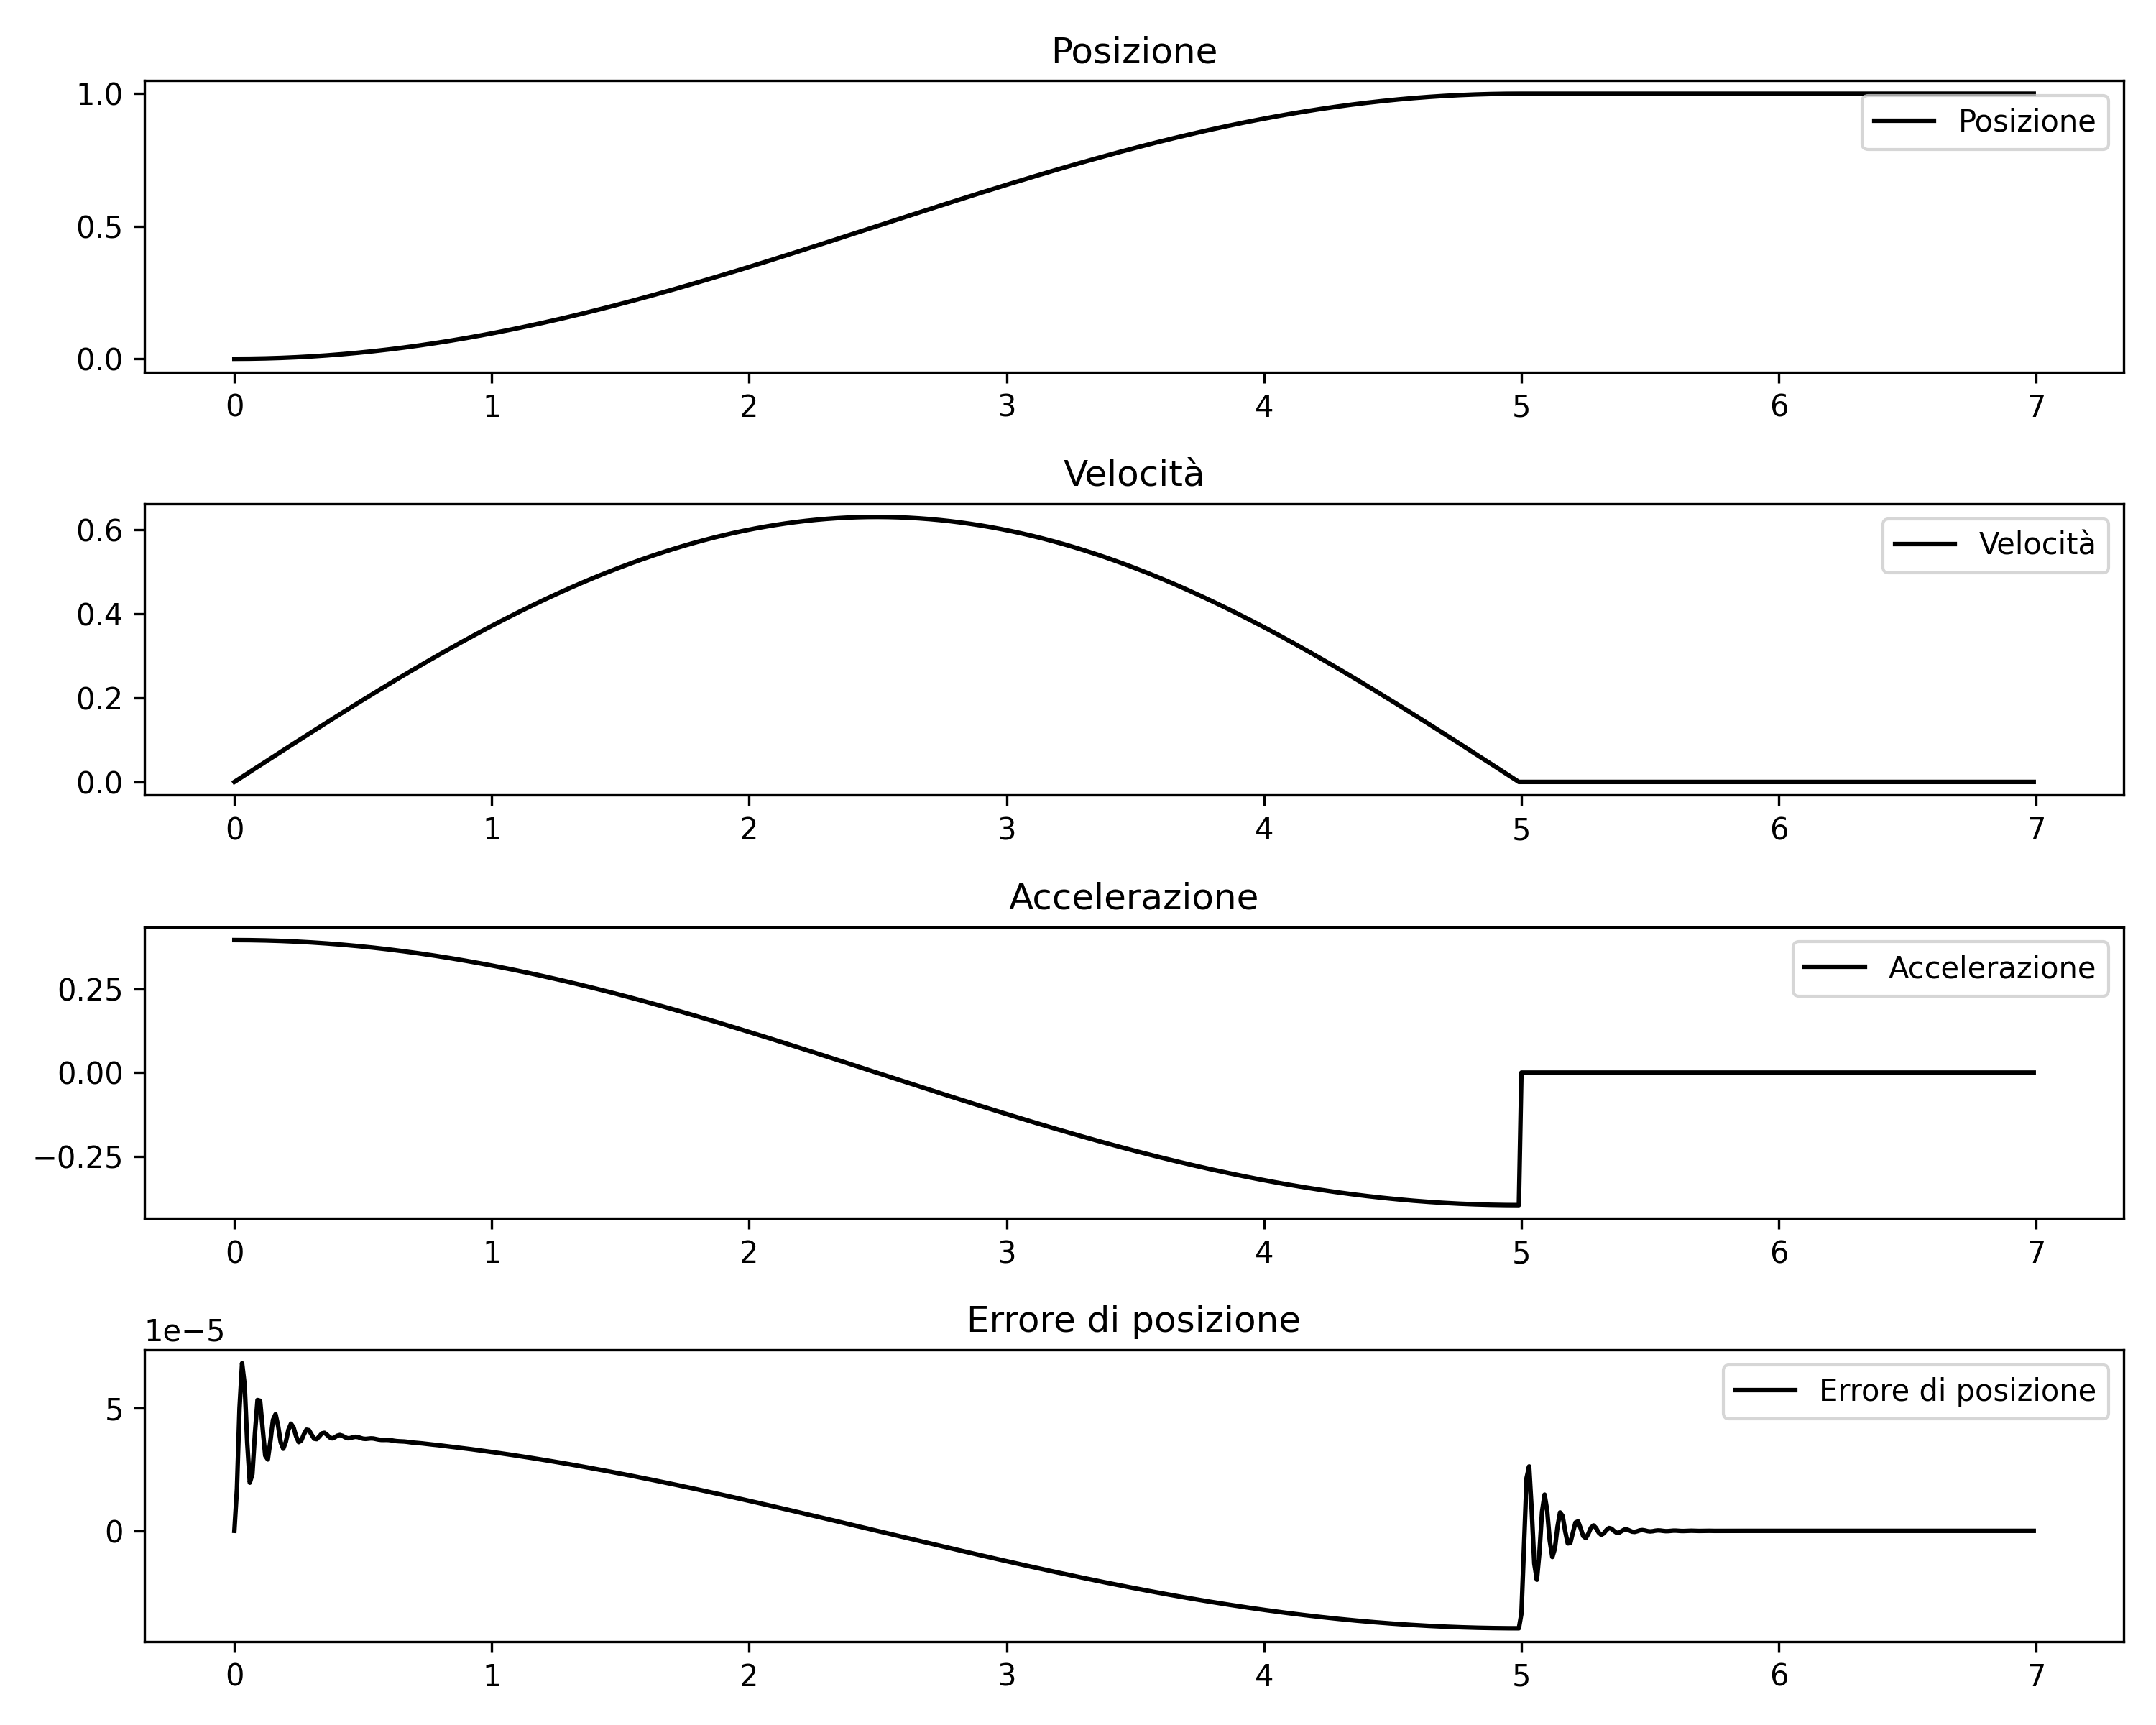
\includegraphics[width=0.45\textwidth]{Immagini/armonica_colocato_v.png}
    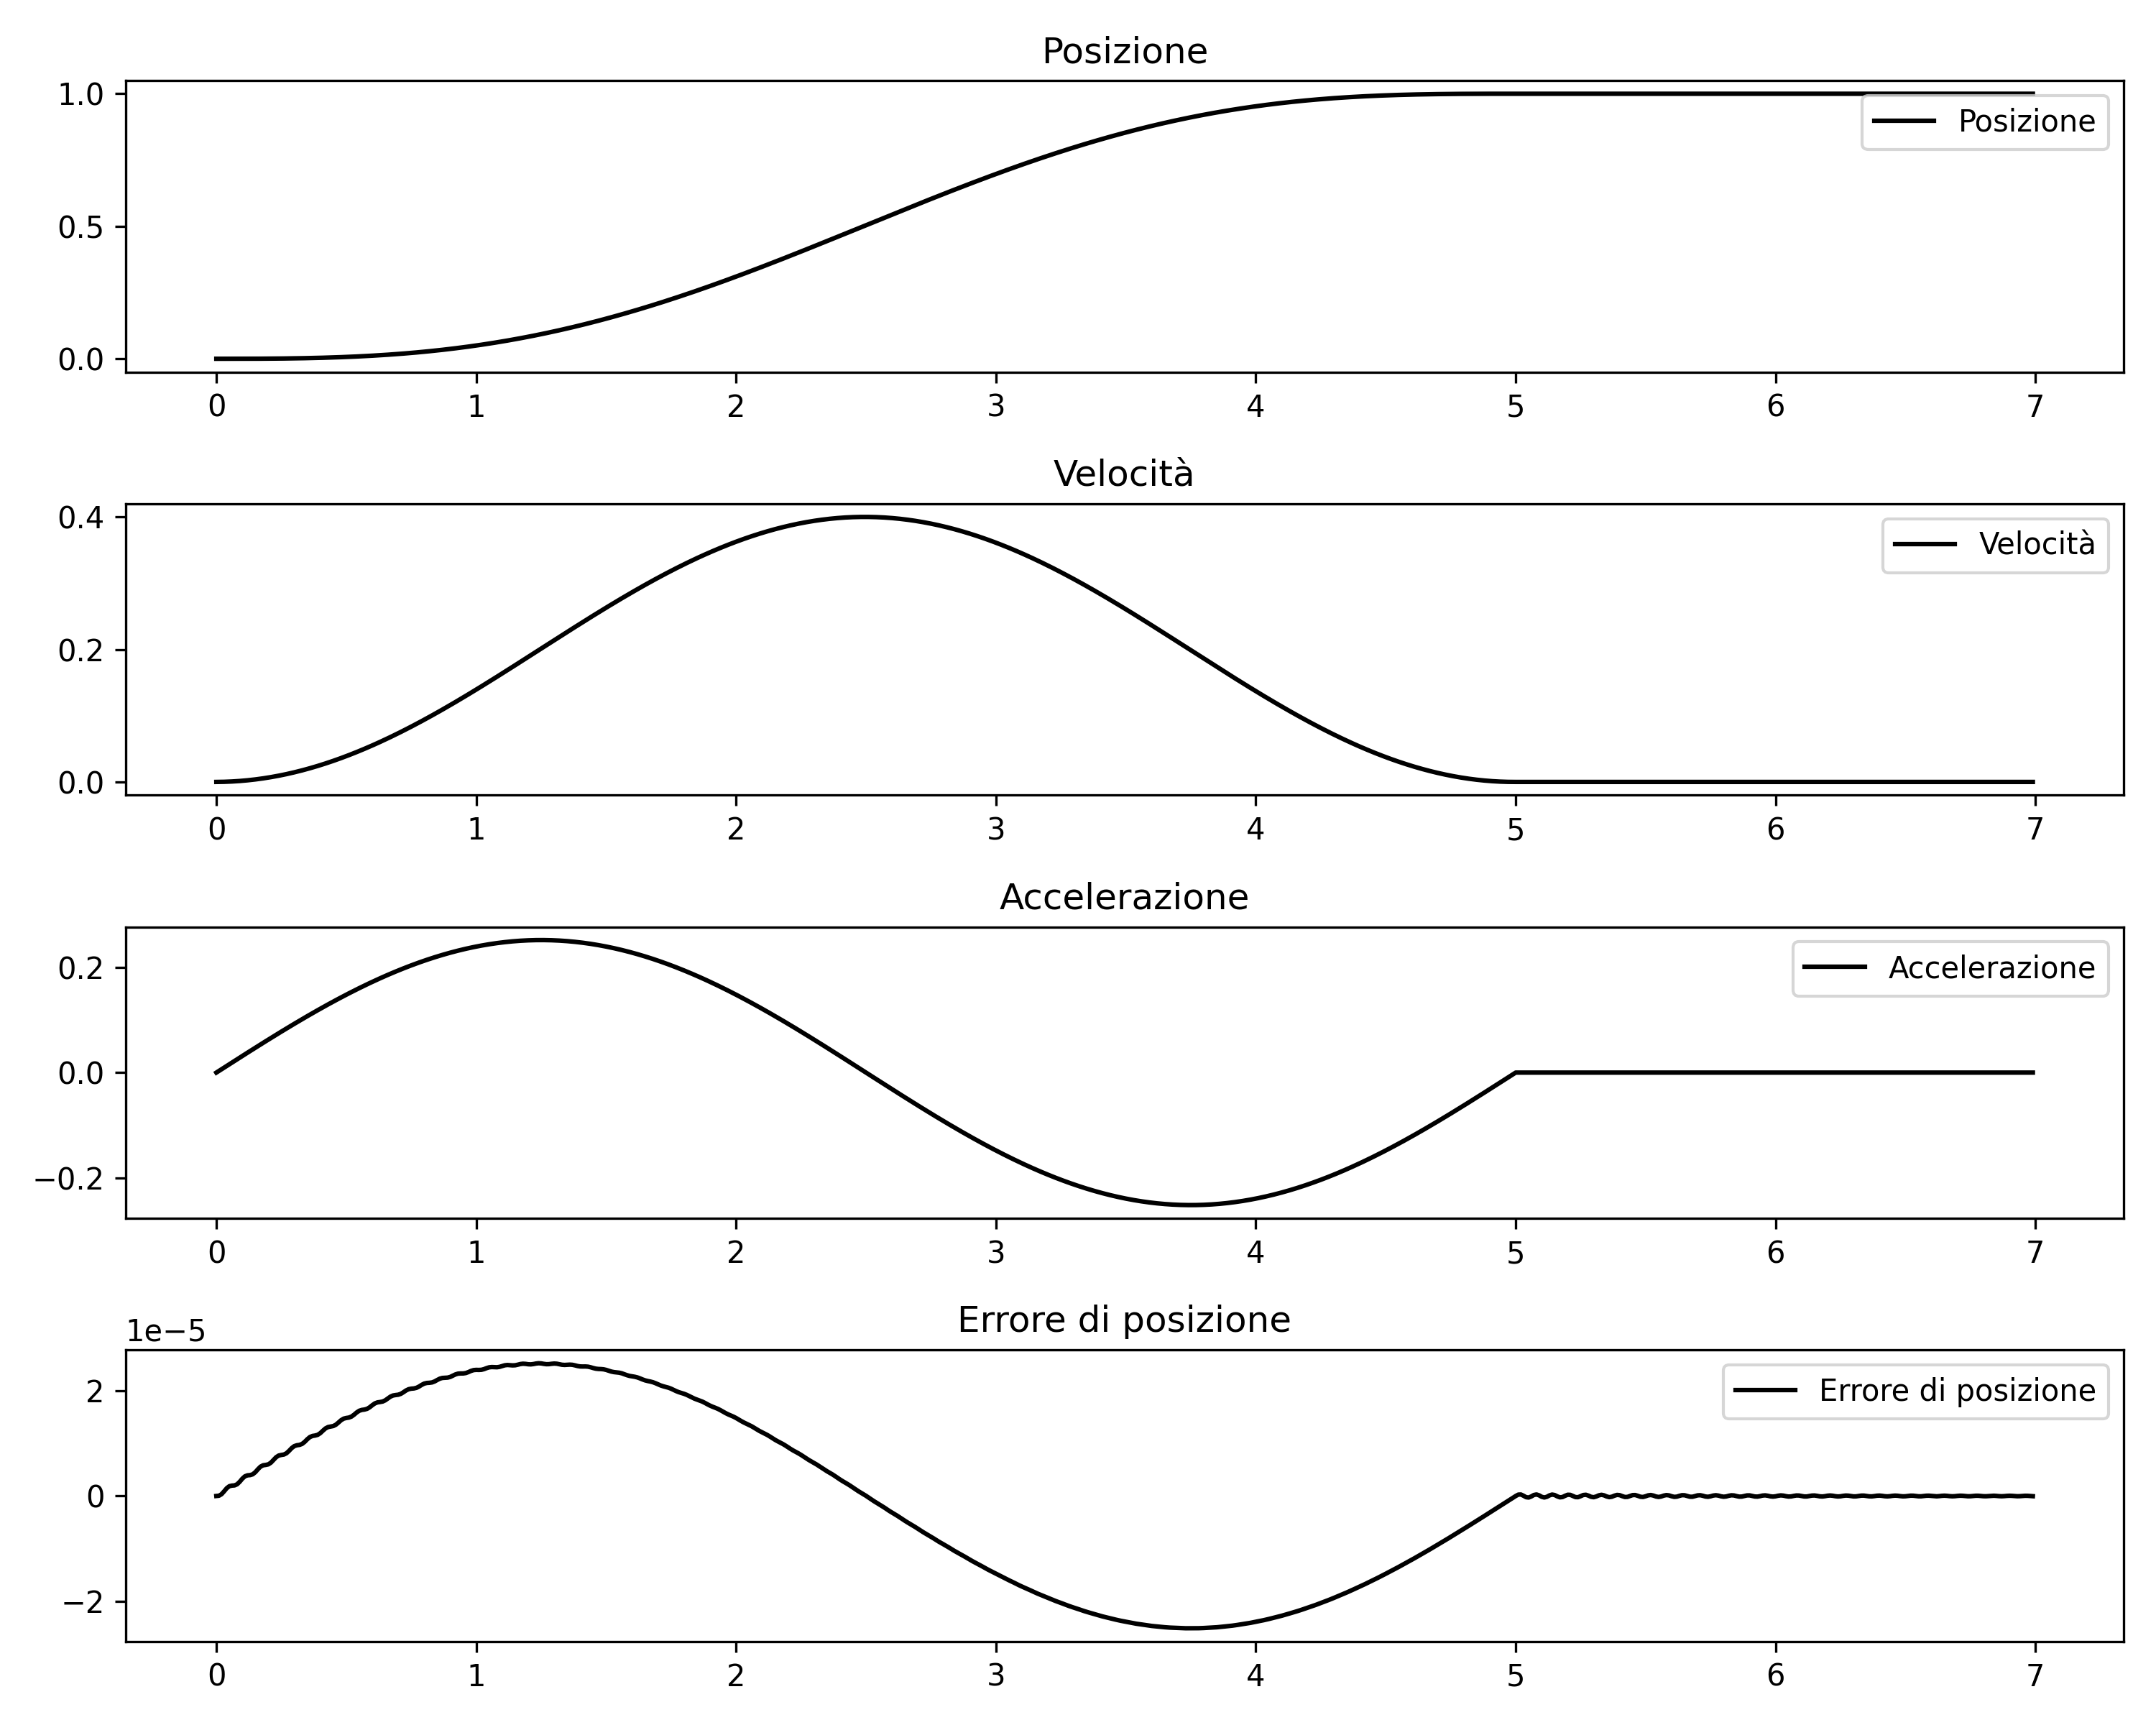
\includegraphics[width=0.45\textwidth]{Immagini/sinusoidale_colocato_v.png}
    \caption{Legge Armonica sx; Sinusoidale in accelerazione dx}
\end{figure}

\sottosezione{Rapporto di inerzia non nullo}
Per \(\rho > 0\) il controllo colocato permette di controllare indirettamente anche il carico.
Questo va diviso in più casi:
\begin{enumerate}
    \item Risonanza in "bassa" frequenza: \(\omega_p << \omega_{tv}, \omega_I\)
    \item Risonanza in "media" frequenza: \(\omega_z \simeq \omega_p \simeq \omega_{tv} \simeq \omega_I\)
    \item Risonanza in "alta" frequenza: \(\omega_z >> \omega_{tv}, \omega_I\)
\end{enumerate} 

\paragrafo{Risonanza in alta frequenza:}
Nel caso di risonanza in alta frequenza (circa un \(\times 2\) tra \(\omega_z\) e \(\omega_{tv},\omega_I\)) non possono essere misurate le oscillazioni dal trasduttore e il motore non può nè eccitare nè controllare le vibrazioni ad alta frequenza. Questo è il caso di un \textbf{equivalente sistema rigido} in cui le risonanza e antirisonanza sono filtrate da trasduttore e anello di corrente, perciò \(G_{vm}(s) \simeq \frac{1}{sJ}\) e l'anello aperto ha funzione di trasferimento \(L(s) \simeq \frac{1}{sJ} C_v K_T H_{trasd} W_I\).

\sottosottosezione{Risonanza in bassa frequenza}
Nel caso di risonanza in bassa frequenza (circa un \(\times 3;4\) tra \(\omega_z\) e \(\omega_{tv}, \omega_I\)) considero intanto il sistema senza gli effetti di trasduttore e anello di corrente che agiscono solo ad alta frequenza, interviene prima l'effetto \textbf{legato alla trasmissione elastica}.
Per facilitare la realizzazione pratica si può considerare la relazione \(\omega_z < \omega_p << \omega_\pi\), perché la pulsazione di attraversamento si verifica, nel controllo colocato, per effetto di trasduttore e anello di corrente.

\paragrafo{Valutazione sulla catena aperta:}
La funzione di trasferimento in catena aperta, dove entrano mobilità, costante di coppia, controllo di velocità, trasduttore e anello di corrente: 
\(L_v(s) = G_{vm}K_T C_v(s) H_{tv}(s) W_I(s)\)
Guardando il Bode dell'anello aperto e confrontandolo con lo stesso sistema in cui vengano trascurati trasduttore e anello di velocità ci si accorge di come abbiano influenza solo in alta frequenza.

\begin{figure}[h]
    \centering
    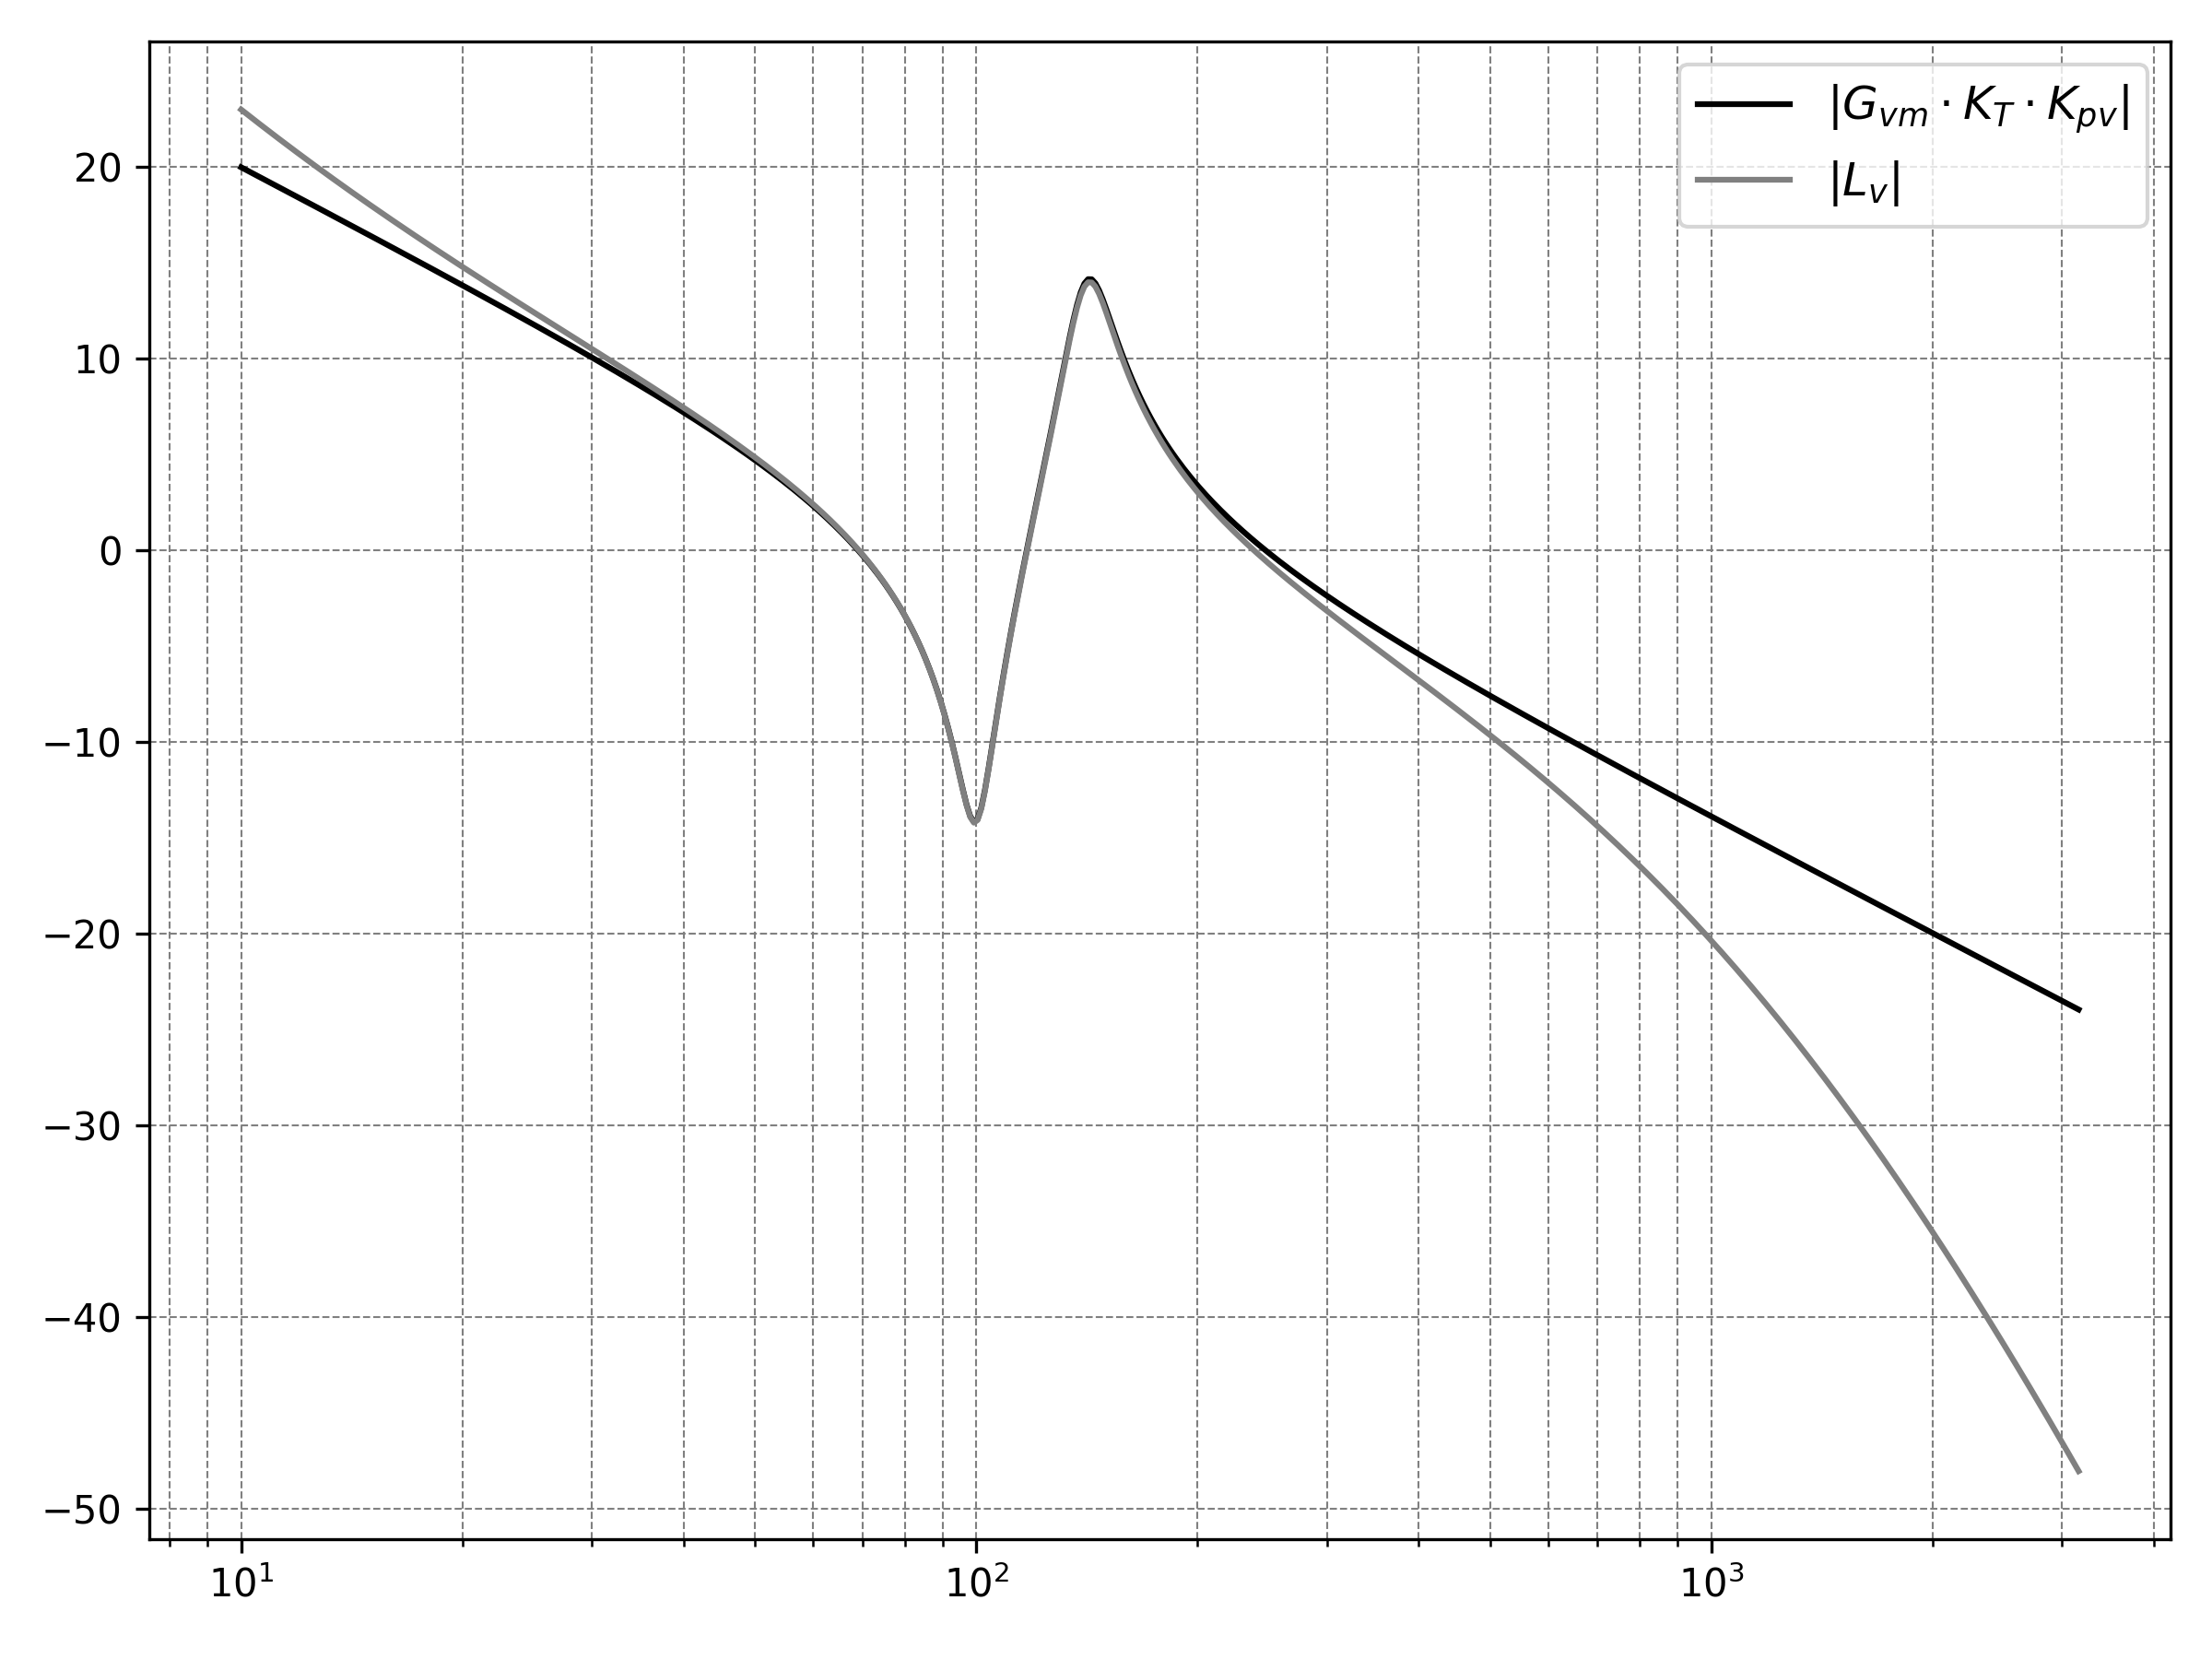
\includegraphics[width=0.35\textwidth]{Immagini/risonanza_bassa_f_Gvm_vs_Lv.png}
    \caption{Effetto di trasduttore e anello di corrente su anello aperto \(L_v\)}
\end{figure}

\paragrafo{Valutazione sulla catena chiusa:}
La funzione di trasferimento in catena chiusa è \(W_v(s) \simeq \frac{G_{vm}C_v K_T}{1+G_{vm}C_v K_T}\), i poli del sistema possono essere analizzati col luogo delle radici (i poli possono essere variati con il \(K_{pv}\)), mentre gli zeri del sistema sono legati a \(G_{vm}C_v\) che ha una coppia di zeri aventi \(\xi_z, \omega_z\), per cui l'antirisonanza della catena chiusa è la stessa di \(G_{vm}\) e uno zero reale \(s=-\frac{1}{T_{iv}}\).

\paragrafo{Con controllore PI:}
Abbiamo visto come il controllo di velocità convenga venire effettuato con controllore PI, di seguito il luogo delle radici in questo caso. A differenza del luogo delle radici con proporzionale si notano il polo nullo e lo zero sull'asse reale.

\begin{figure}[h]
    \centering
    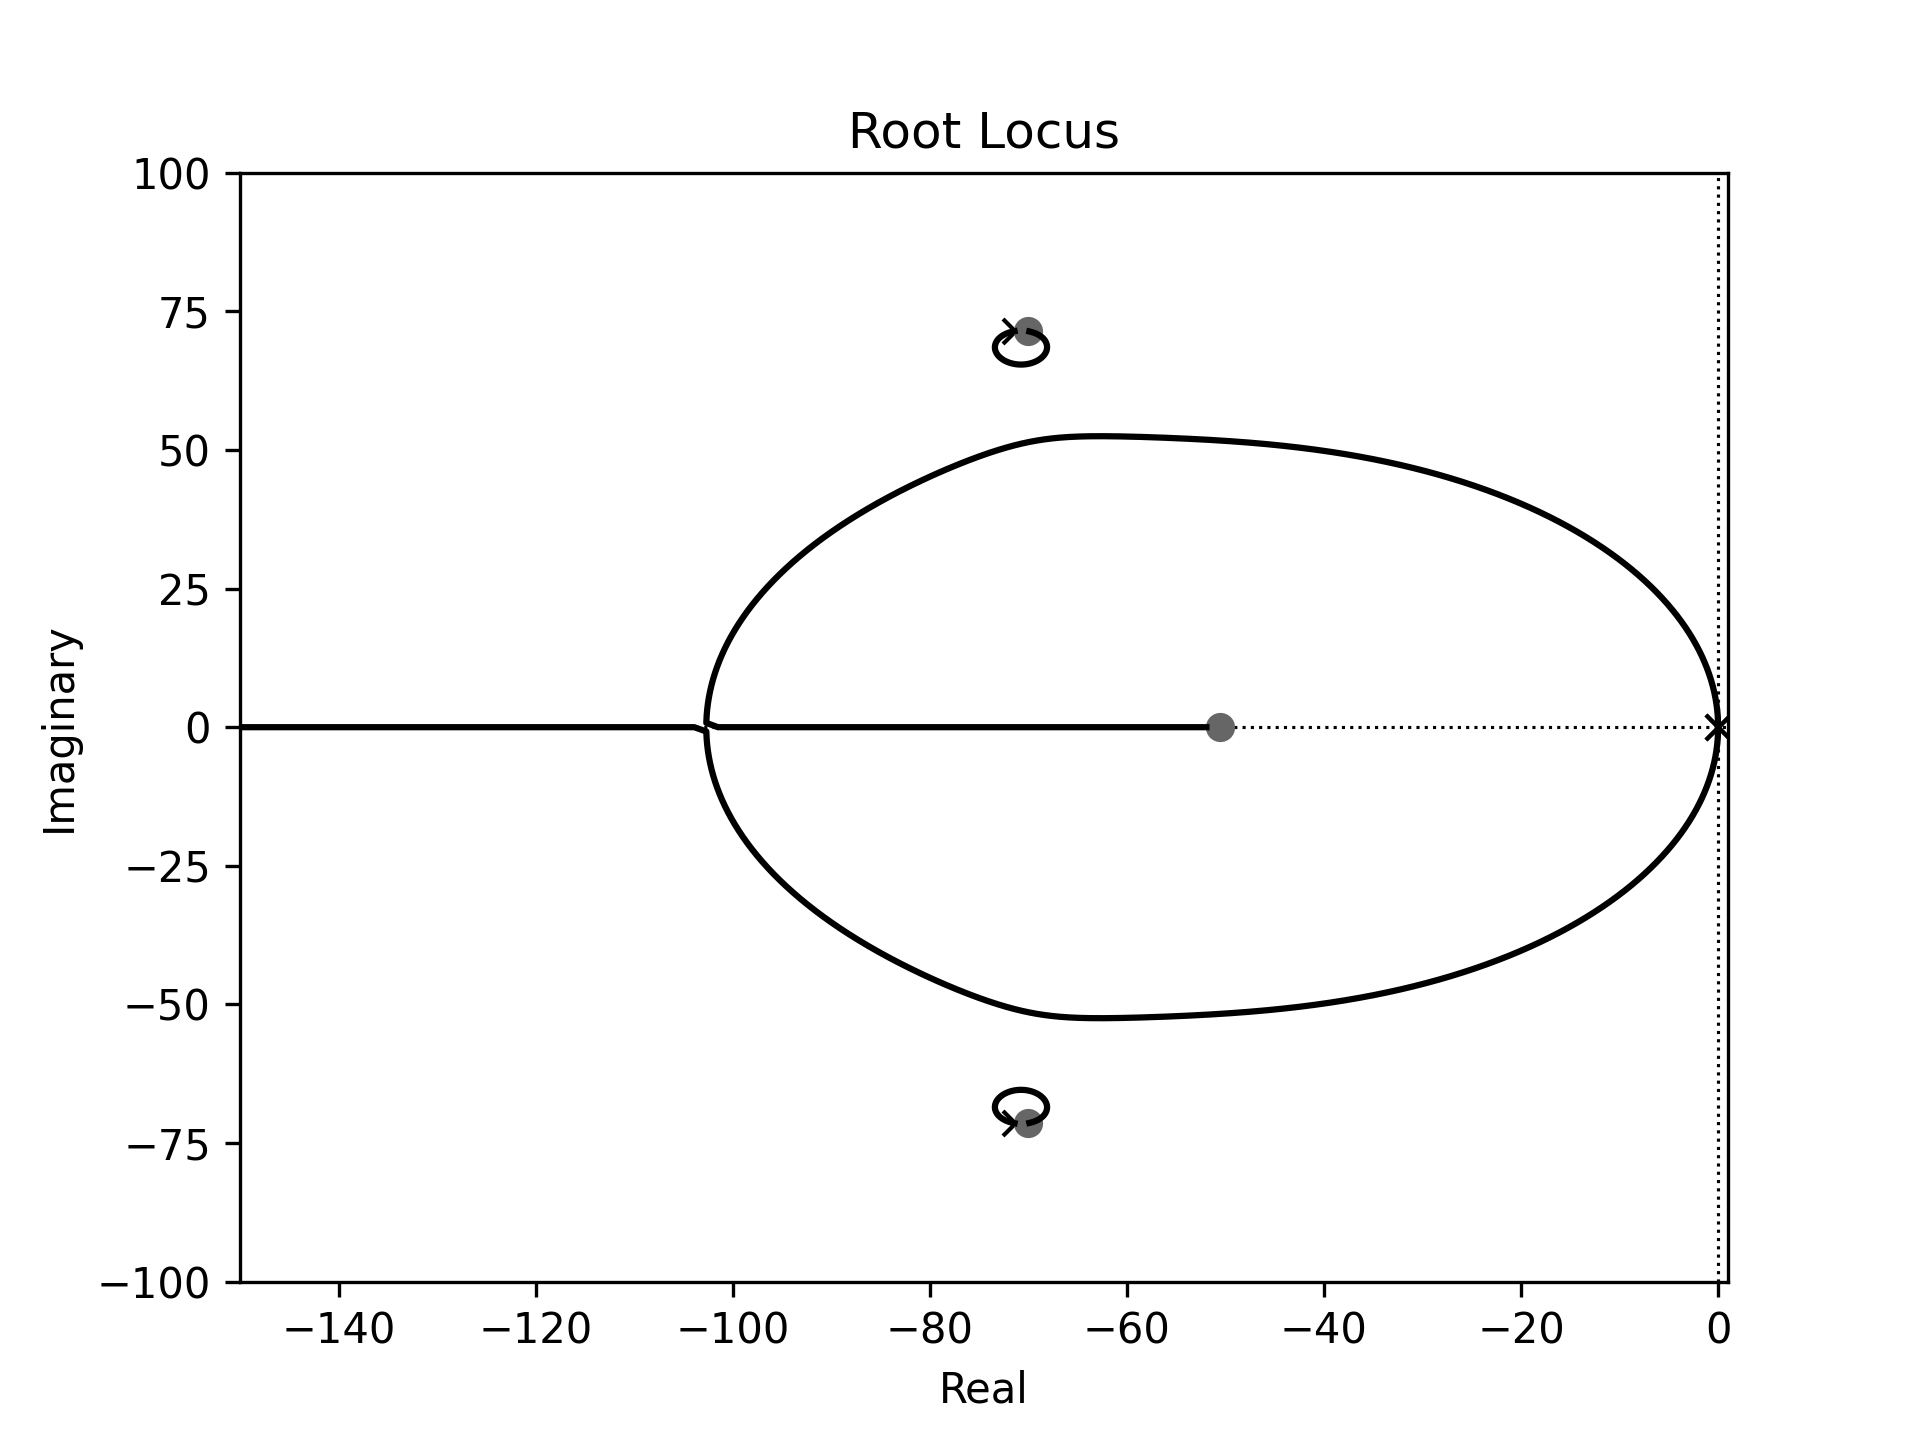
\includegraphics[width=0.4\textwidth]{Immagini/controllo_v_colocato_PI.png}
    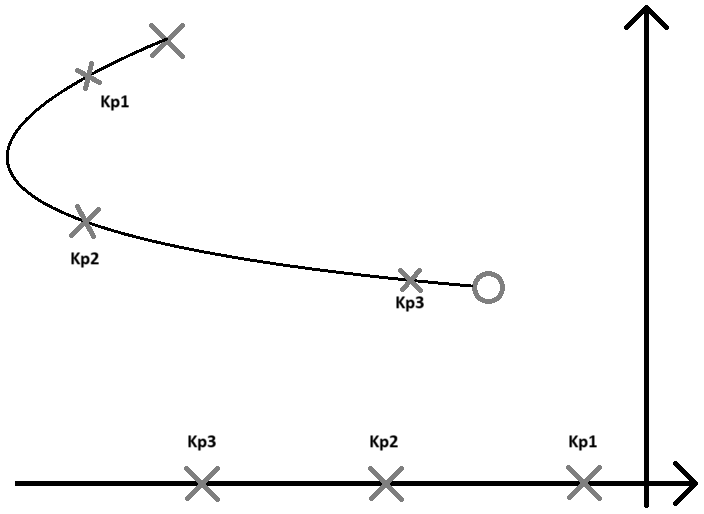
\includegraphics[width=0.35\textwidth]{Immagini/rlocus_vari_guadagni_controlloVel_PI.png}
    \caption{Controllo Colocato con controllore PI sx; guadagni \(K_{pv1},K_{pv2},K_{pv3}\) dx}
\end{figure}

\paragrafo{Tipici approcci di progetto:}
Fissato \(\omega_{bv}^{des} \simeq [0.5\div 0.7]\omega_z\), calcolo, approssimando il sistema ad un sistema rigido \footnote{Perchè considero di lavorare prima di risonanza e antirisonanza.}: \(K_{pv} \simeq \frac{\omega_{bv}^{des} J}{K_T}\) e \(\frac{1}{T_{iv}} \simeq \frac{\omega_{bv}^{des}}{4 \xi_{des}^2}\) con smorzamento del polo del sistema a catena chiusa \(\xi_{des} \geqslant 1\) (perché non conviene rischiare avendo trasmissione elastica).
Alternativamente è possibile partire considerando il luogo delle radici, e cercare \(K_{pv}\) tale che siano massimizzati \(\xi_\text{poli}\) o \(\mathbb{R}(\text{poli})\).
I due metodi portano a \(K_{pv}\) paragonabili e nella zona di ottimo.
Tenendo a mente che rimane da garantire \footnote{Vedi \ref{Teq} per condizioni per sistema con trasmissione rigida.} \(\omega_{bv} > \frac{\frac{1}{T_{eq}}}{4\xi^2}\).

\sottoparagrafo{Scelta del guadagno:}
Per quanto riguarda \(K_{pv}\), ci sono le seguenti tipologie di situazioni:
\begin{itemize}
    \item \(K_{pv,1}\) guadagno "basso": Un basso guadagno porta ad avere \(\omega_{bv}\) "bassa" perché viene fatta una scelta di parte reale non ottima, che porta ad uno smorzamento non ottimale \footnote{Per valutare la stabilità col luogo delle radici si considera la distanza dall'asse immaginario (più distante più stabile) in combinazione col valore di \(\alpha\), quindi di \(\xi\).}
    \item \(K_{pv,2}\) guadagno "ottimale": Un guadagno ottimale è associato ad una scelta di \(\xi\) massimo, quindi parte reale massima e \(\omega_{bv} < \omega_z\)
    \item \(K_{pv,3}\) guadagno "alto": Un guadagno alto porta ad avere una cancellazione polo zero, quindi una buona compensazione dell'antirisonanza
\end{itemize}

\paragrafo{Valutazioni sul carico:}
Il picco di risonanza della trasmissibilità "compensa" il picco di antirisonanza di \(W_v\), lato carico si ottiene un \(\omega_{bv}\) maggiore.
Bisogna quindi prestare attenzione a utilizzare guadagni troppo elevati (caso \(K_{pv,3}\)) perché, sebbene il motore possa beneficiarne, potrebbe portare ad avere una eccessiva compensazione, causata dalla trasmissibilità, lato carico, portando ad avere in uscita picchi di risonanza.
Per guadagno ottimale, invece, avere \(\omega_{bv} < \omega_z\), permette alla trasmissibilità di compensare bene l'antirisonanza, quindi lato carico si ottiene una buona risposta con una banda passante "grande".

\begin{figure}[h]
    \centering
    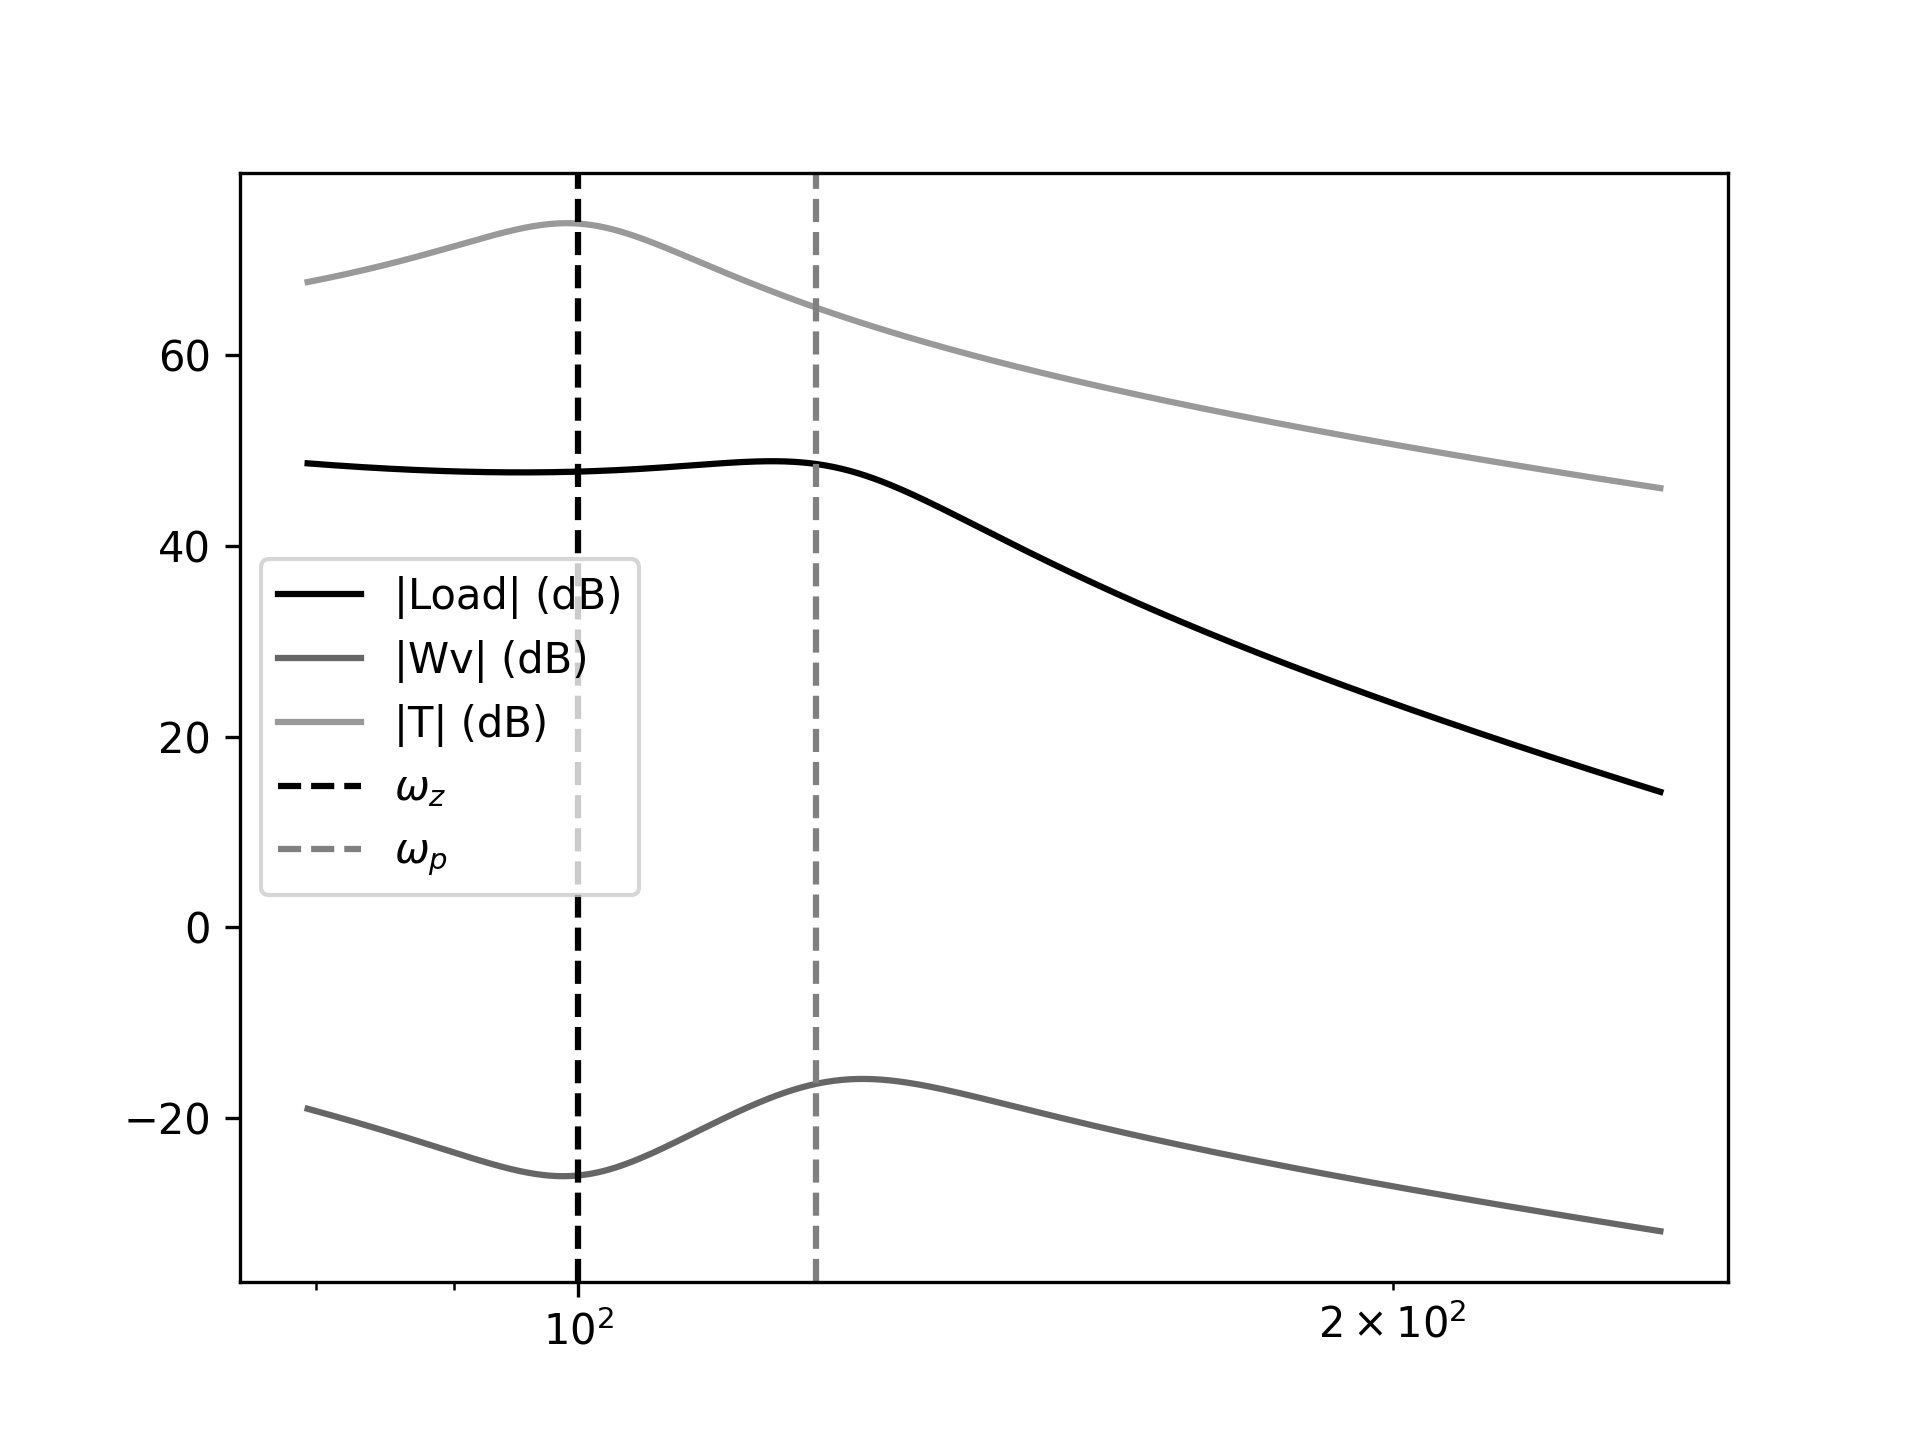
\includegraphics[width=0.45\textwidth]{Immagini/colocato_v_lato_carico.png}
    \caption{Effetto di compensazione dell'antirisonanza}
\end{figure}

\paragrafo{Risposta al gradino per vari guadagni:}
La risposta al gradino per un sistema che abbia impostato un guadagno \(K_{pv,2}\) "ottimo" \footnote{Nè troppo elevato, per cui lato carico si ottenga picco di risonanza per eccesso di compensazione, nè troppo ridotto, per cui si ottenga una bassa banda passante} ha una sovraelongazione dovuta allo zero a causa della scelta del gradino come legge di moto, ma carico e motore mantengono andamenti simili.
La risposta al gradino per un sistema che abbia impostato un guadagno \(K_{pv,3}\) "troppo elevato" vede grandi oscillazioni sia al motore sia al carico, che potrebbero avere andamenti differenti e peggiori al carico.

\begin{figure}[h]
    \centering
    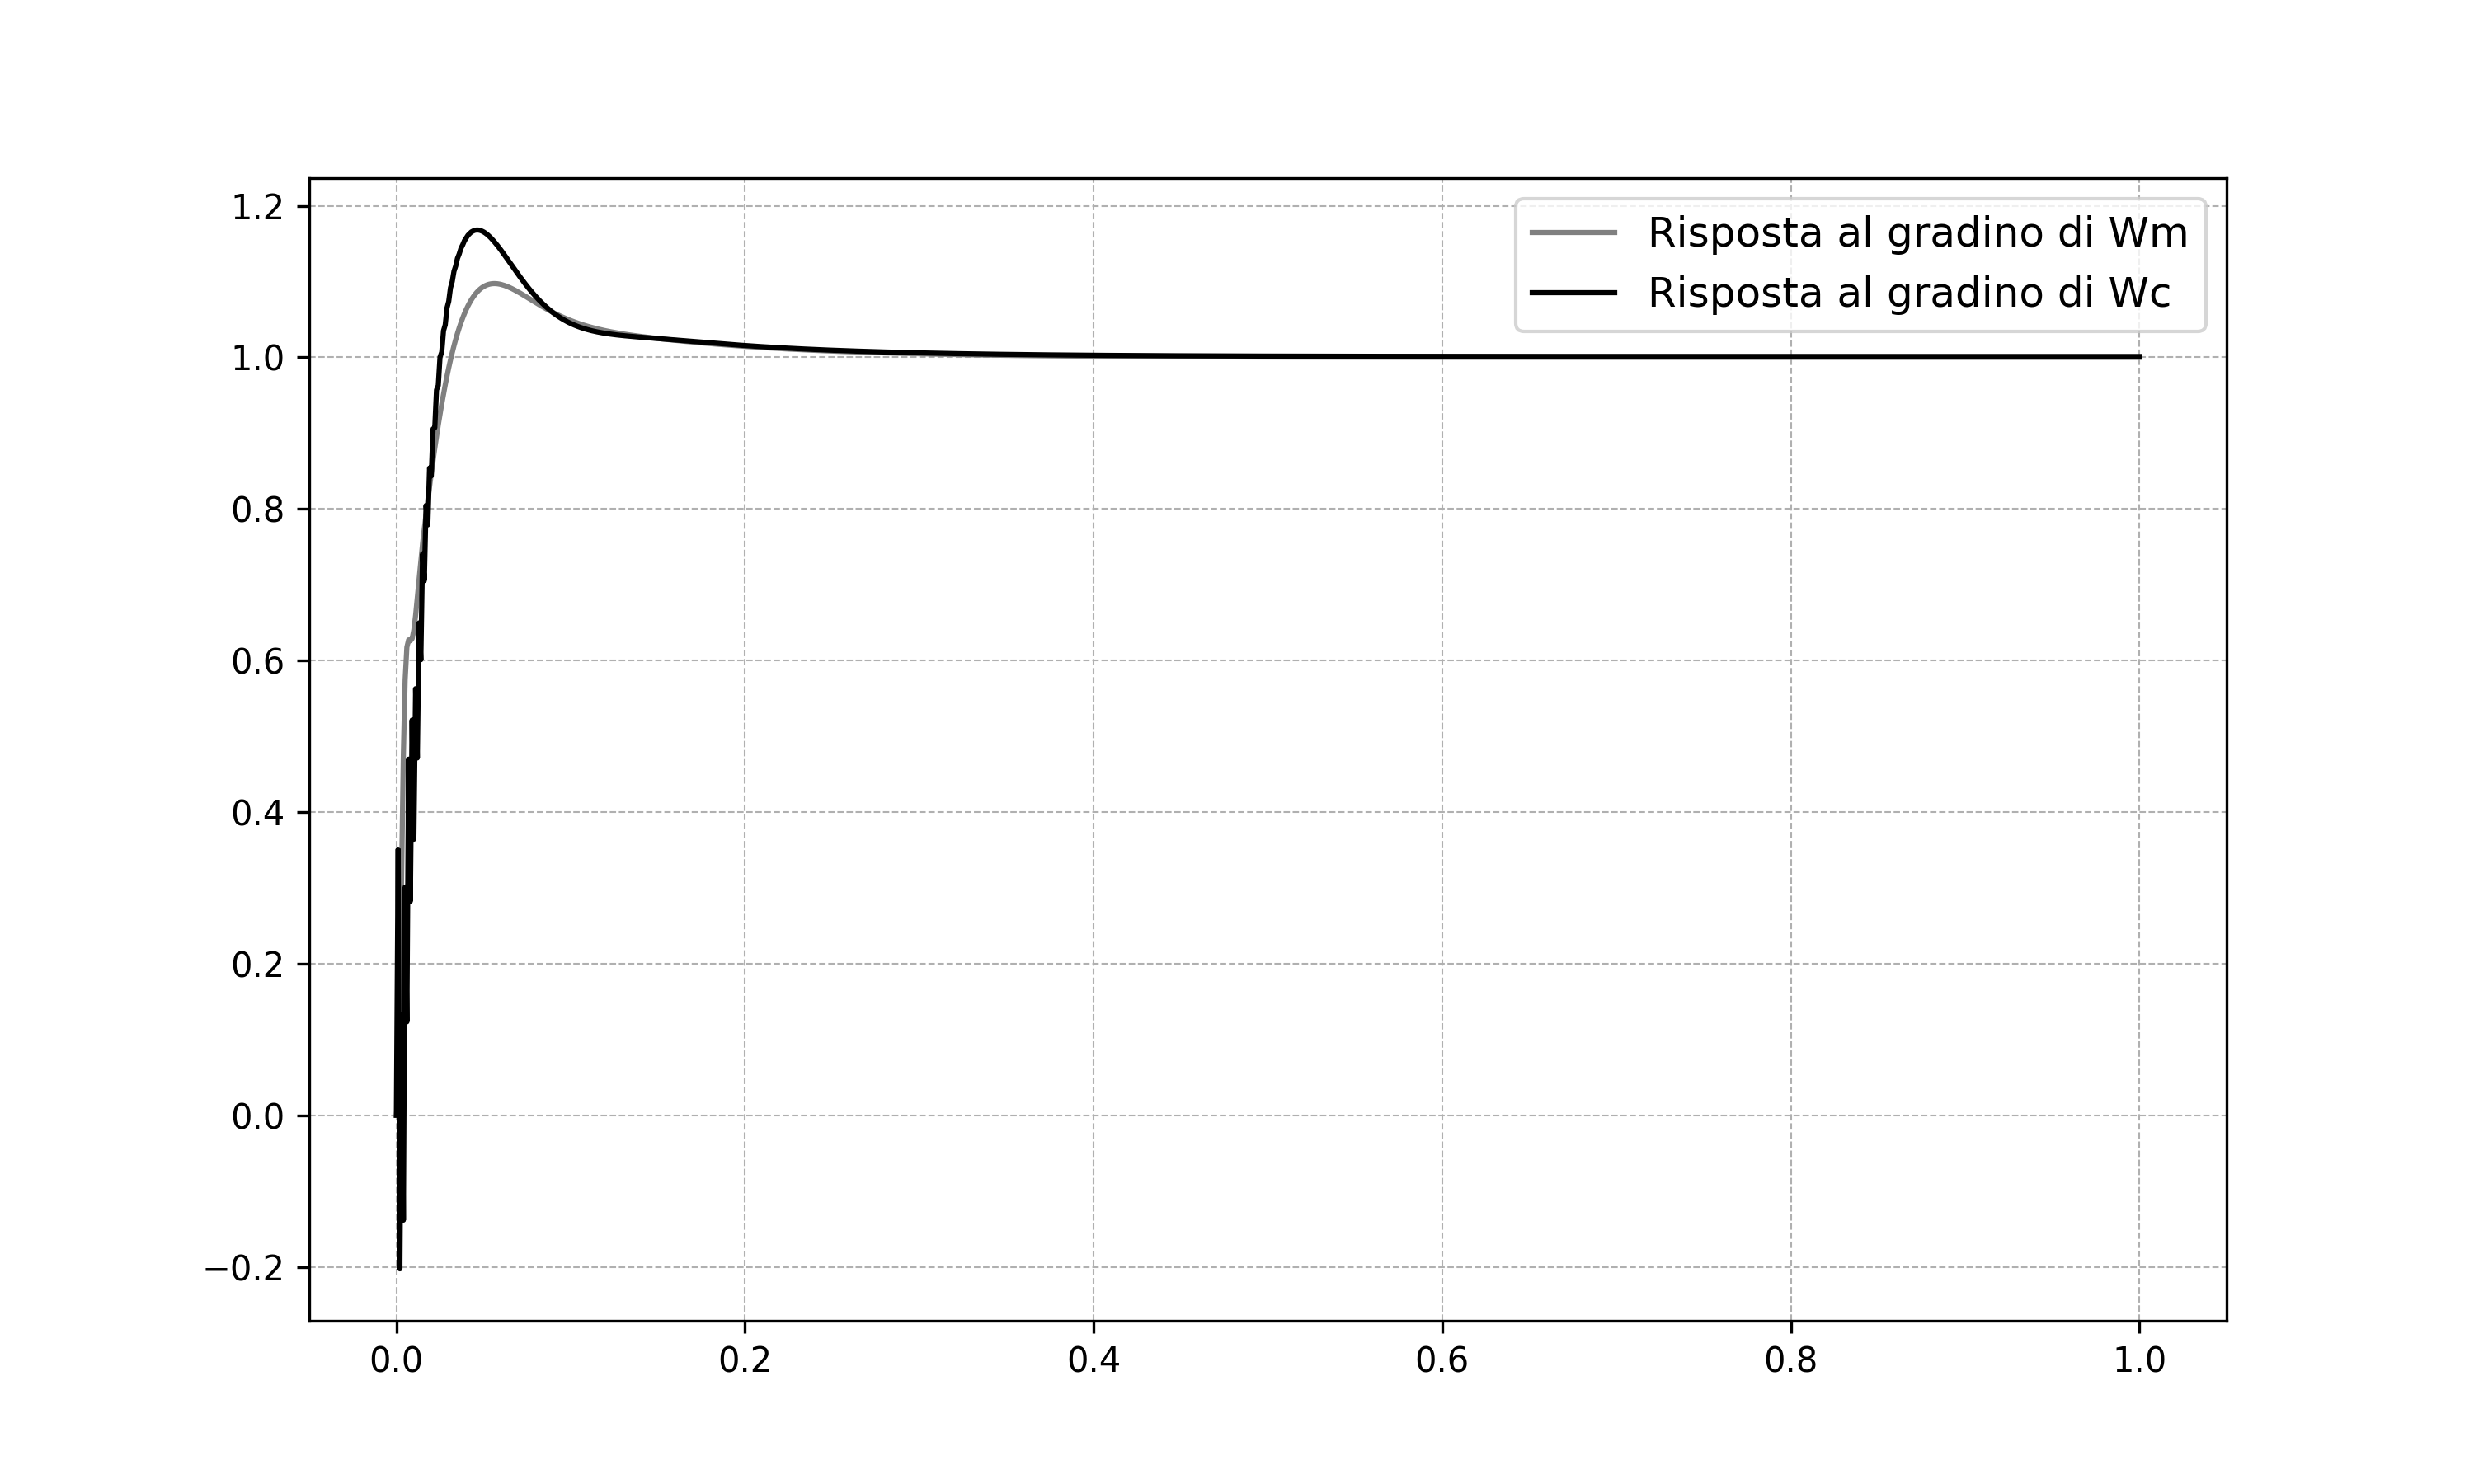
\includegraphics[width=0.4\textwidth]{Immagini/step_response_Kp2.png}
    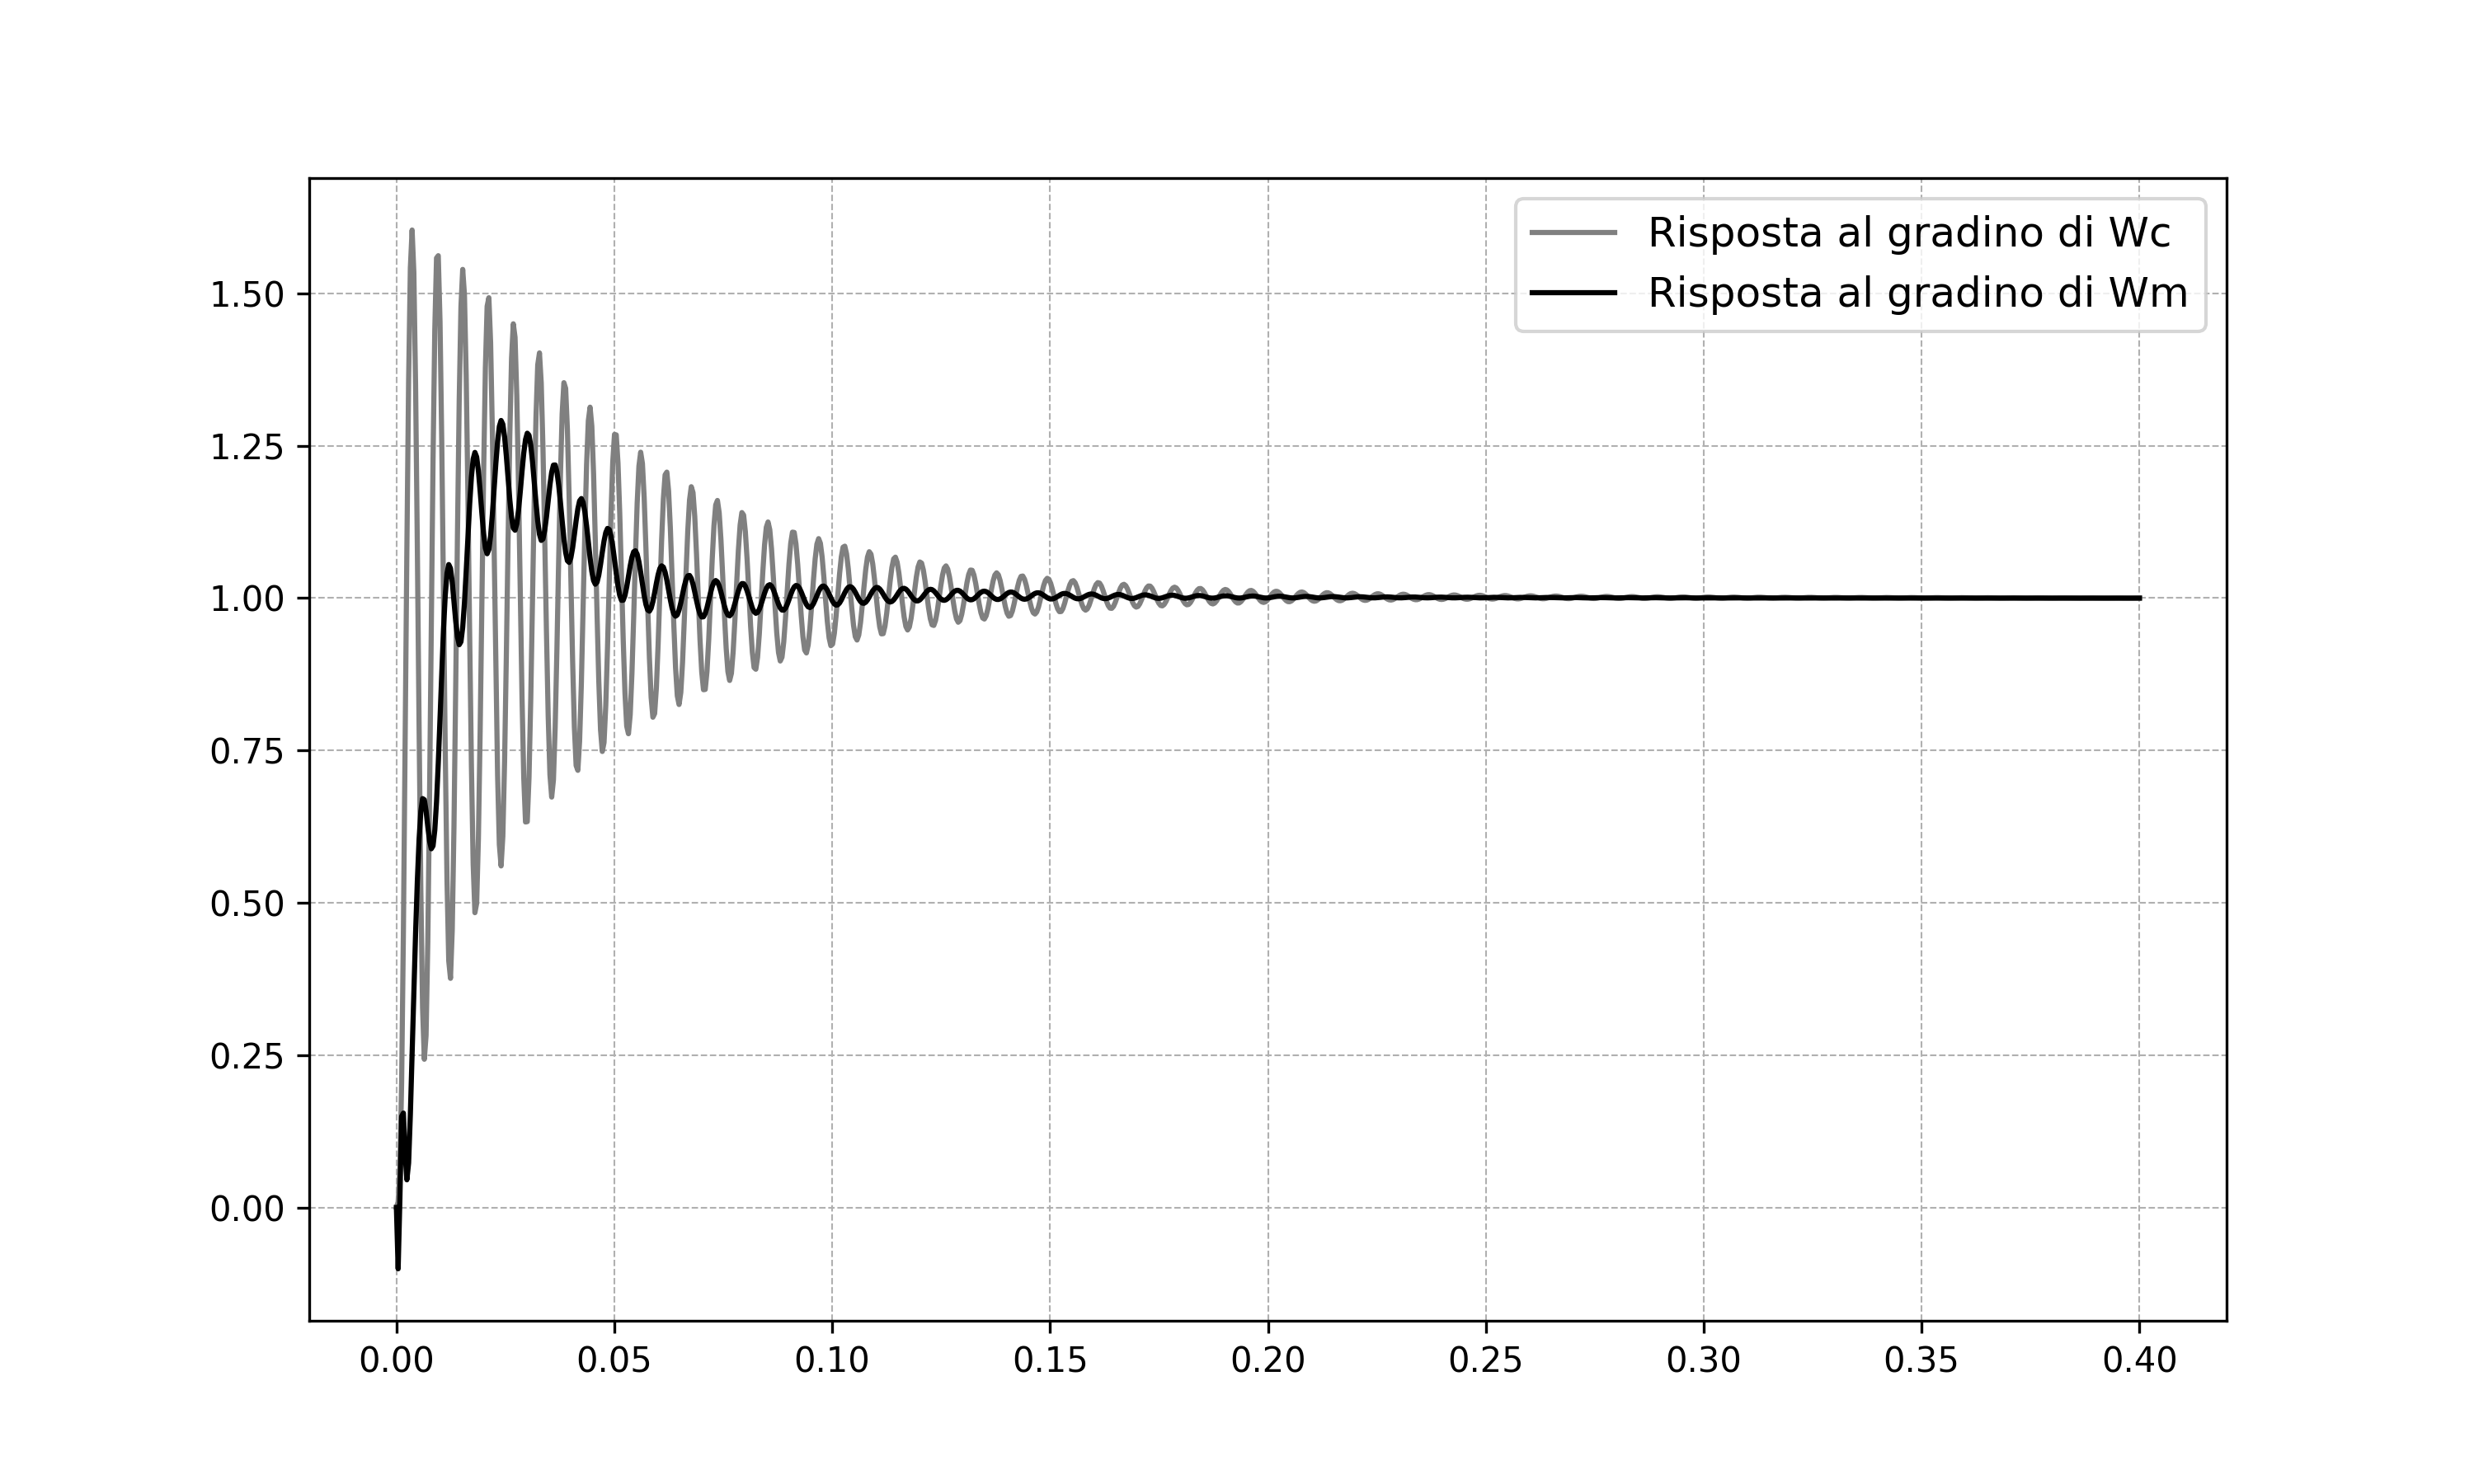
\includegraphics[width=0.4\textwidth]{Immagini/step_response_Kp3.png}
    \caption{Risposte al gradino \(K_{p2}\) sx, \(K_{p3}\) dx (inversione colori per questioni grafiche)}
\end{figure}

\sottosottosezione{Risonanza in media frequenza}
Avere risonanza in media frequenza significa \(\omega_z,\omega_p \simeq \omega_{tv},\omega_I,\omega_\pi\). Questo caso è il più complicato da gestire perché non esiste una regola euristica, il sistema non è nè sufficientemente rigido da poter fare l'analisi come visto nel capitolo precedente, nè sufficientemente elastico per poter considerare la risonanza in bassa frequenza.
La causa di questa complessità è legata alla presenza, in prossimità di \(\omega_p\), di una serie di poli che portano in catena aperta, \(L_v\), a perdita repentina di fase, portando ad avere in uno degli attraversamenti margine di fase negativo, ossia ad avere sistema instabile.

\begin{figure}[h]
    \centering
    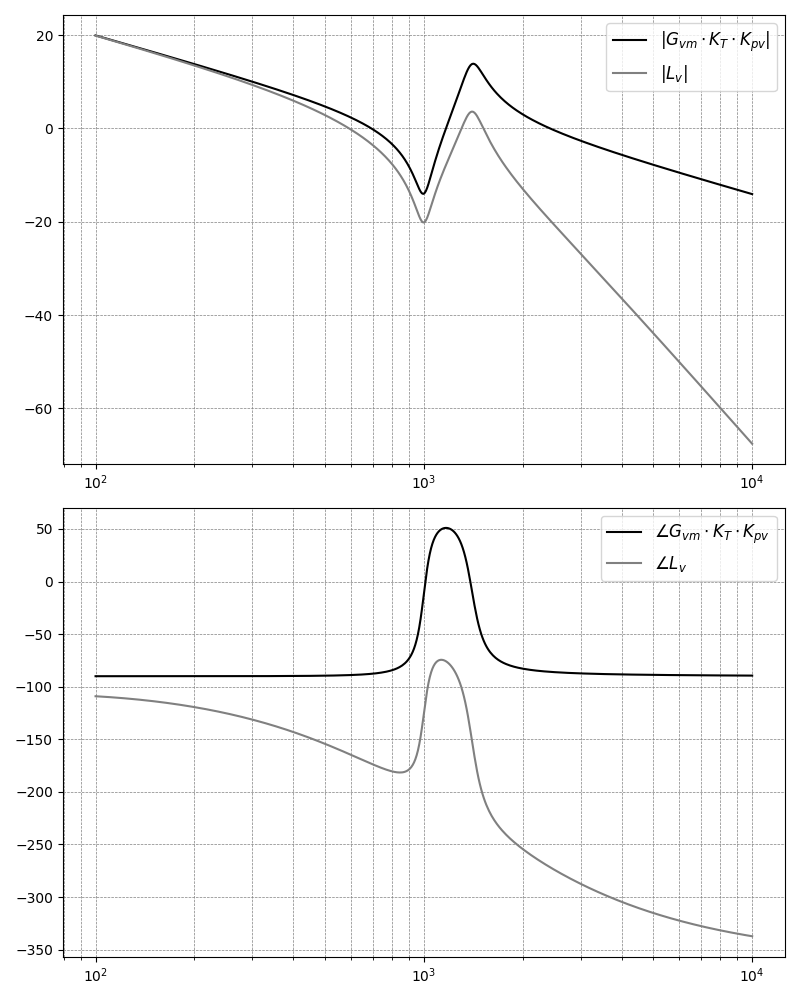
\includegraphics[width=0.35\textwidth]{Immagini/risonanza_media_f_Gvm_vs_Lv.png}
    \caption{Effetto trasduttore e anello di corrente su anello aperto \(L_v\)}
\end{figure}

\paragrafo{Soluzioni:}
Ci sono diverse possibili soluzioni attuabili, che considerano il controllo, il progetto e la meccanica.
\begin{enumerate}[label=\roman*.]
    \item Riduzione del guadagno \(\downarrow K_{pv}\): Questo permette di abbassare il modulo di \(L_v\) andando a "eliminare" le pulsazioni di attraversamento indesiderate. Tuttavia "eliminare" la risonanza richiede guadagni molto bassi, che portano ad avere banda passante bassa \(\downarrow \omega_{bv}\), compensabile con leggi di moto dolci e feedforward.
    In alternativa, volendo essere meno conservativi, è possibile tarare sul sistema\footnote{Vedi autotuning {\color{red} Aggiungere riferimento appena disponibile}} il valore di \(K_{pv}\) tale che si ottenga l'attraversamento in un punto in cui il margine di fase sia sufficiente, portando ad avere una banda passante maggiore. Questo secondo approccio però è rischioso, perché il cambio di fase può essere molto rapido e variazioni minime del guadagno possono avere conseguente disastrose sul sistema.
    \item Aumento di \(\omega_{tv}\), scelta di trasduttore con risoluzione maggiore: Il trasduttore è solitamente l'elemento critico, perciò sceglierne uno con risoluzione maggiore permette di spostare la frequenza di taglio del filtro. Scegliere encoder sin/cos, in combinazione con una \(K_{pv}\) "bassa" (rispetto quello che avrei per un sistema rigido), permette di considerare l'amplificazione del rumore trascurabile.
    \textbf{Attenzione}: utilizzare uno stimatore di velocità che non consideri l'elasticità, potrebbe portare a problemi soprattutto in stima di accelerazione dove lo stimatore lavora in alta frequenza.
    \item Aumento di \(\omega_I\): Solitamente il trasduttore è l'elemento critico in questi sistemi, tuttavia migliorare il trasduttore potrebbe portare l'anello di corrente ad essere il nuovo elemento critico.
    \item Aumento della rigidezza del riduttore: La rigidezza del riduttore influenza le pulsazioni di antirisonanza \(\omega_z = \sqrt{\frac{k}{J_c}}\) e risonanza \(\omega_p = \sqrt{\frac{k}{J_c}}\sqrt{1+\rho}\), tuttavia la presenza della radice porta ad un minor effetto, un aumento considerevole di rigidezza (comunque difficile da ottenere), non porta grandi benefici al sistema. 
    \item Rapporto di inerzia minore, \(\downarrow \rho\): Utilizzare \(\downarrow \rho\) fa sì che vi sia cancellazione polo-zero \(\omega_z,\omega_p\) in \(G_{vm}, L_v\), risultando in una perdita di pulsazioni di attraversamento indesiderate, o comunque in uno spostamento in frequenza degli attraversamenti, lontano da fase critica. \textbf{Nel caso di risonanza in media frequenza, lavorare con rapporto di inerzia ridotto è spesso il modo più semplice per facilitare il controllo lato motore. Occorre poi fare una pianificazione del moto ad hoc per il carico.}
    Come fare a variare il rapporto di inerzia \(\rho = \frac{\tau_R^2 J_c}{J_M}\):
        \begin{enumerate}[label=\alph*)]
            \item Se possibile diminuendo l'inerzia lato carico, prestando attenzione che \(J_c\) influenza \(\rho\), ma anche \(\omega_z\) e \(\omega_p\)
            \item Diminuendo il rapporto di trasmissione \(\downarrow \tau_R\), tenendo conto che questo porta a perdita dell'ottimo in termini di coppia, velocità, energia e che i riduttori multistadio sono caratterizzati da maggior \(\uparrow\) gioco e ridotta rigidezza \(\downarrow k\). Potrebbe avere senso utilizzare riduttori di nuovo tipo, vedi \ref{riduttori_speciali}.
            \item Utilizzo di volano lato motore di modo da aumentare il denominatore, però così facendo aumenta la taglia del motore, il progetto risulta sovradimensionato, e soprattutto aggiungere alberi e una massa porta ad aggiunta di risonanza e antirisonanza meccanica.
            \item Utilizzo di motori ad alta inerzia, sono costruttivamente diffenti rispetto i motori tradizionali, hanno un raggio maggiore e lunghezza minore, così \(J_M \uparrow \propto R^4 \) (perché si considera a parità di densità volumetrica). Questa è una alternativa al volano, risulta comunque inefficiente.
            \item Modifica virtuale di \(\rho\) con tecniche di controllo fornite dal costruttore:
            \begin{enumerate}
                \item Load observer (Rockwell, Bechoff)
                \item Acceleration Feedback (Kollmorgen)
            \end{enumerate}
        \end{enumerate}
        \item Utilizzo di filtri tra controllo di velocità e anello di corrente:
        In modo del tutto simile al caso con trasmissione rigida (vedi {\color{red} Aggiungere riferimento}), i filtri possono essere consideranti all'interno del \(T_{eq} = \frac{1}{\omega_{tv}}+\frac{1}{\omega_I}+\frac{T_c}{2}+\dots + \frac{1}{\omega_\text{b,filtro}}\), e dato che anche in questo caso si può considerare \(\omega_{bv}\simeq \frac{\frac{1}{T_{eq}}}{4}\), considerando il fattore 4 che li lega, dovrà valere: \[\omega_\text{b,filtro} > \omega_{bv} \cdot 4\]
        \begin{enumerate}[label=\alph*)]
            \item Passa basso: Il più semplice, tuttavia occorre tener conto della perdita di fase associata.
            Per valutarne l'efficacia occorre conoscere il tipo di filtro passa basso utilizzato e soprattutto l'ordine del filtro, che ha conseguenze positive in modulo, perché va a attenuare il picco di risonanza, ma negative in fase, che potrebbe portare ad instabilità.
            \item Filtri notch: Vedi in seguito
            \item Reti anticipatrici: Porta aumento di fase, che però si associa ad una amplificazione del modulo, perciò va a spostare l'attraversamento per pulsazioni superiori, dove la fase è peggiore, e amplifica rumore e disturbi.
            \item BIQUAD: Vedi in seguito
        \end{enumerate}
\end{enumerate}

\sottoparagrafo{Filtro Notch:}
Il filtro notch serve ad attenuare una specifica pulsazione, l'idea è quella di fase una cancellazione polo zero con \(G_{vm}\), di modo da poter scegliere lo smorzamento del polo complessivo. Nella pratica \(\xi_p,\xi_d\) diventano parametri di ottimizzazione del controllo.
La funzione di trasferimento associata al filtro è \(F(s) = \frac{\frac{s^2}{\omega_p^2} + \frac{2\xi_p}{\omega_p}s + 1}{\frac{s^2}{\omega_p^2} + \frac{2\xi_d}{\omega_p}s + 1}\):
\begin{itemize}
    \item Richiede conoscenza di \(\omega_p\)
    \item Ha fase negativa per \(\omega < \omega_p\)
    \item Richiede di avere \(\omega_p\) poco variabile (per esempio, non è adatto per viti a ricircolo di sfere in cui la pulsazione varia con la posizione della chiocciola)
    \item Fissato \(\xi_p\), aumentare \(\xi_d\) porta ad un aumento dell'attenuazione e allargamento della banda di attenuazione, ma anche ad un maggior disturbo in fase
    \item Fissato \(\frac{\xi_d}{\xi_p}\), vengono mantenute costante l'attenuazione e l'entità del disturbo in fase, aumentare \(\xi_p\) porta ad allargamento della banda di attenuazione e allargamento del disturbo di fase
    \item Fissato \(\xi_d\) che mantiene fissata la largezza di banda di attenuazione, aumentare \(\xi_p\) porta a riduzione dell'attenuazione e riduzione del disturbo in fase
\end{itemize}

\begin{figure}[h]
    \centering
    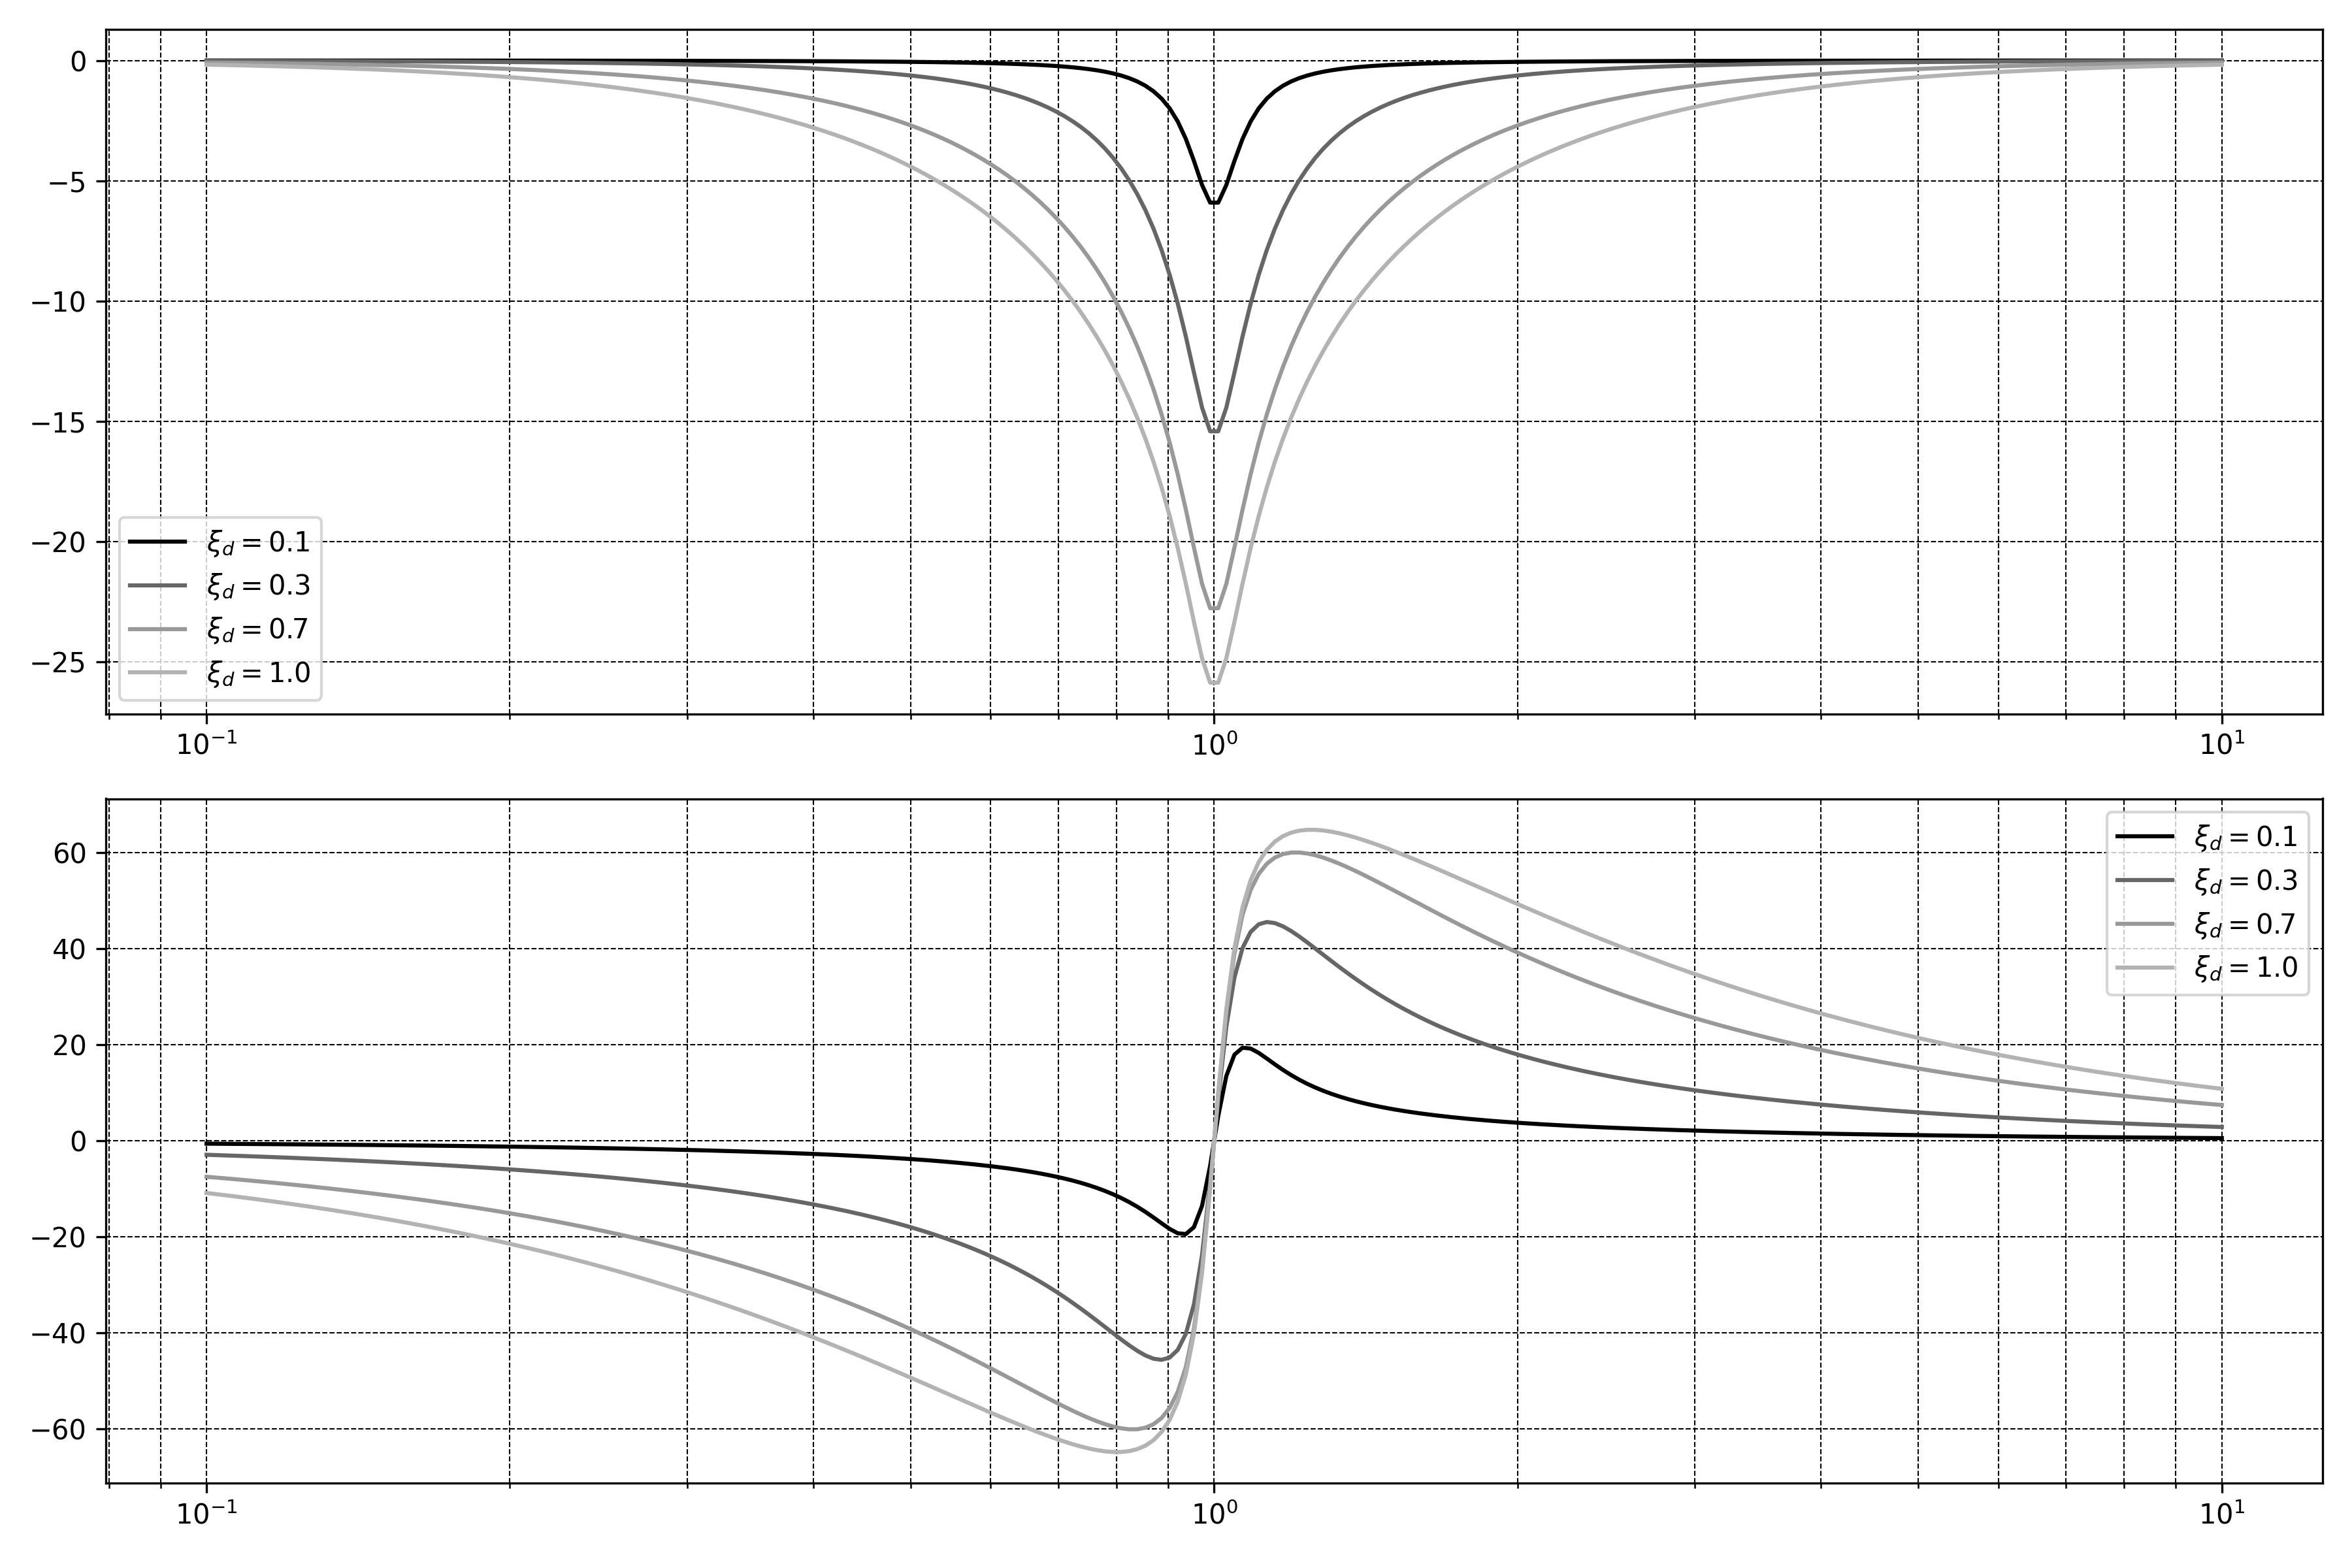
\includegraphics[width=0.3\textwidth]{Immagini/filtro_notch_xip_costante.png}
    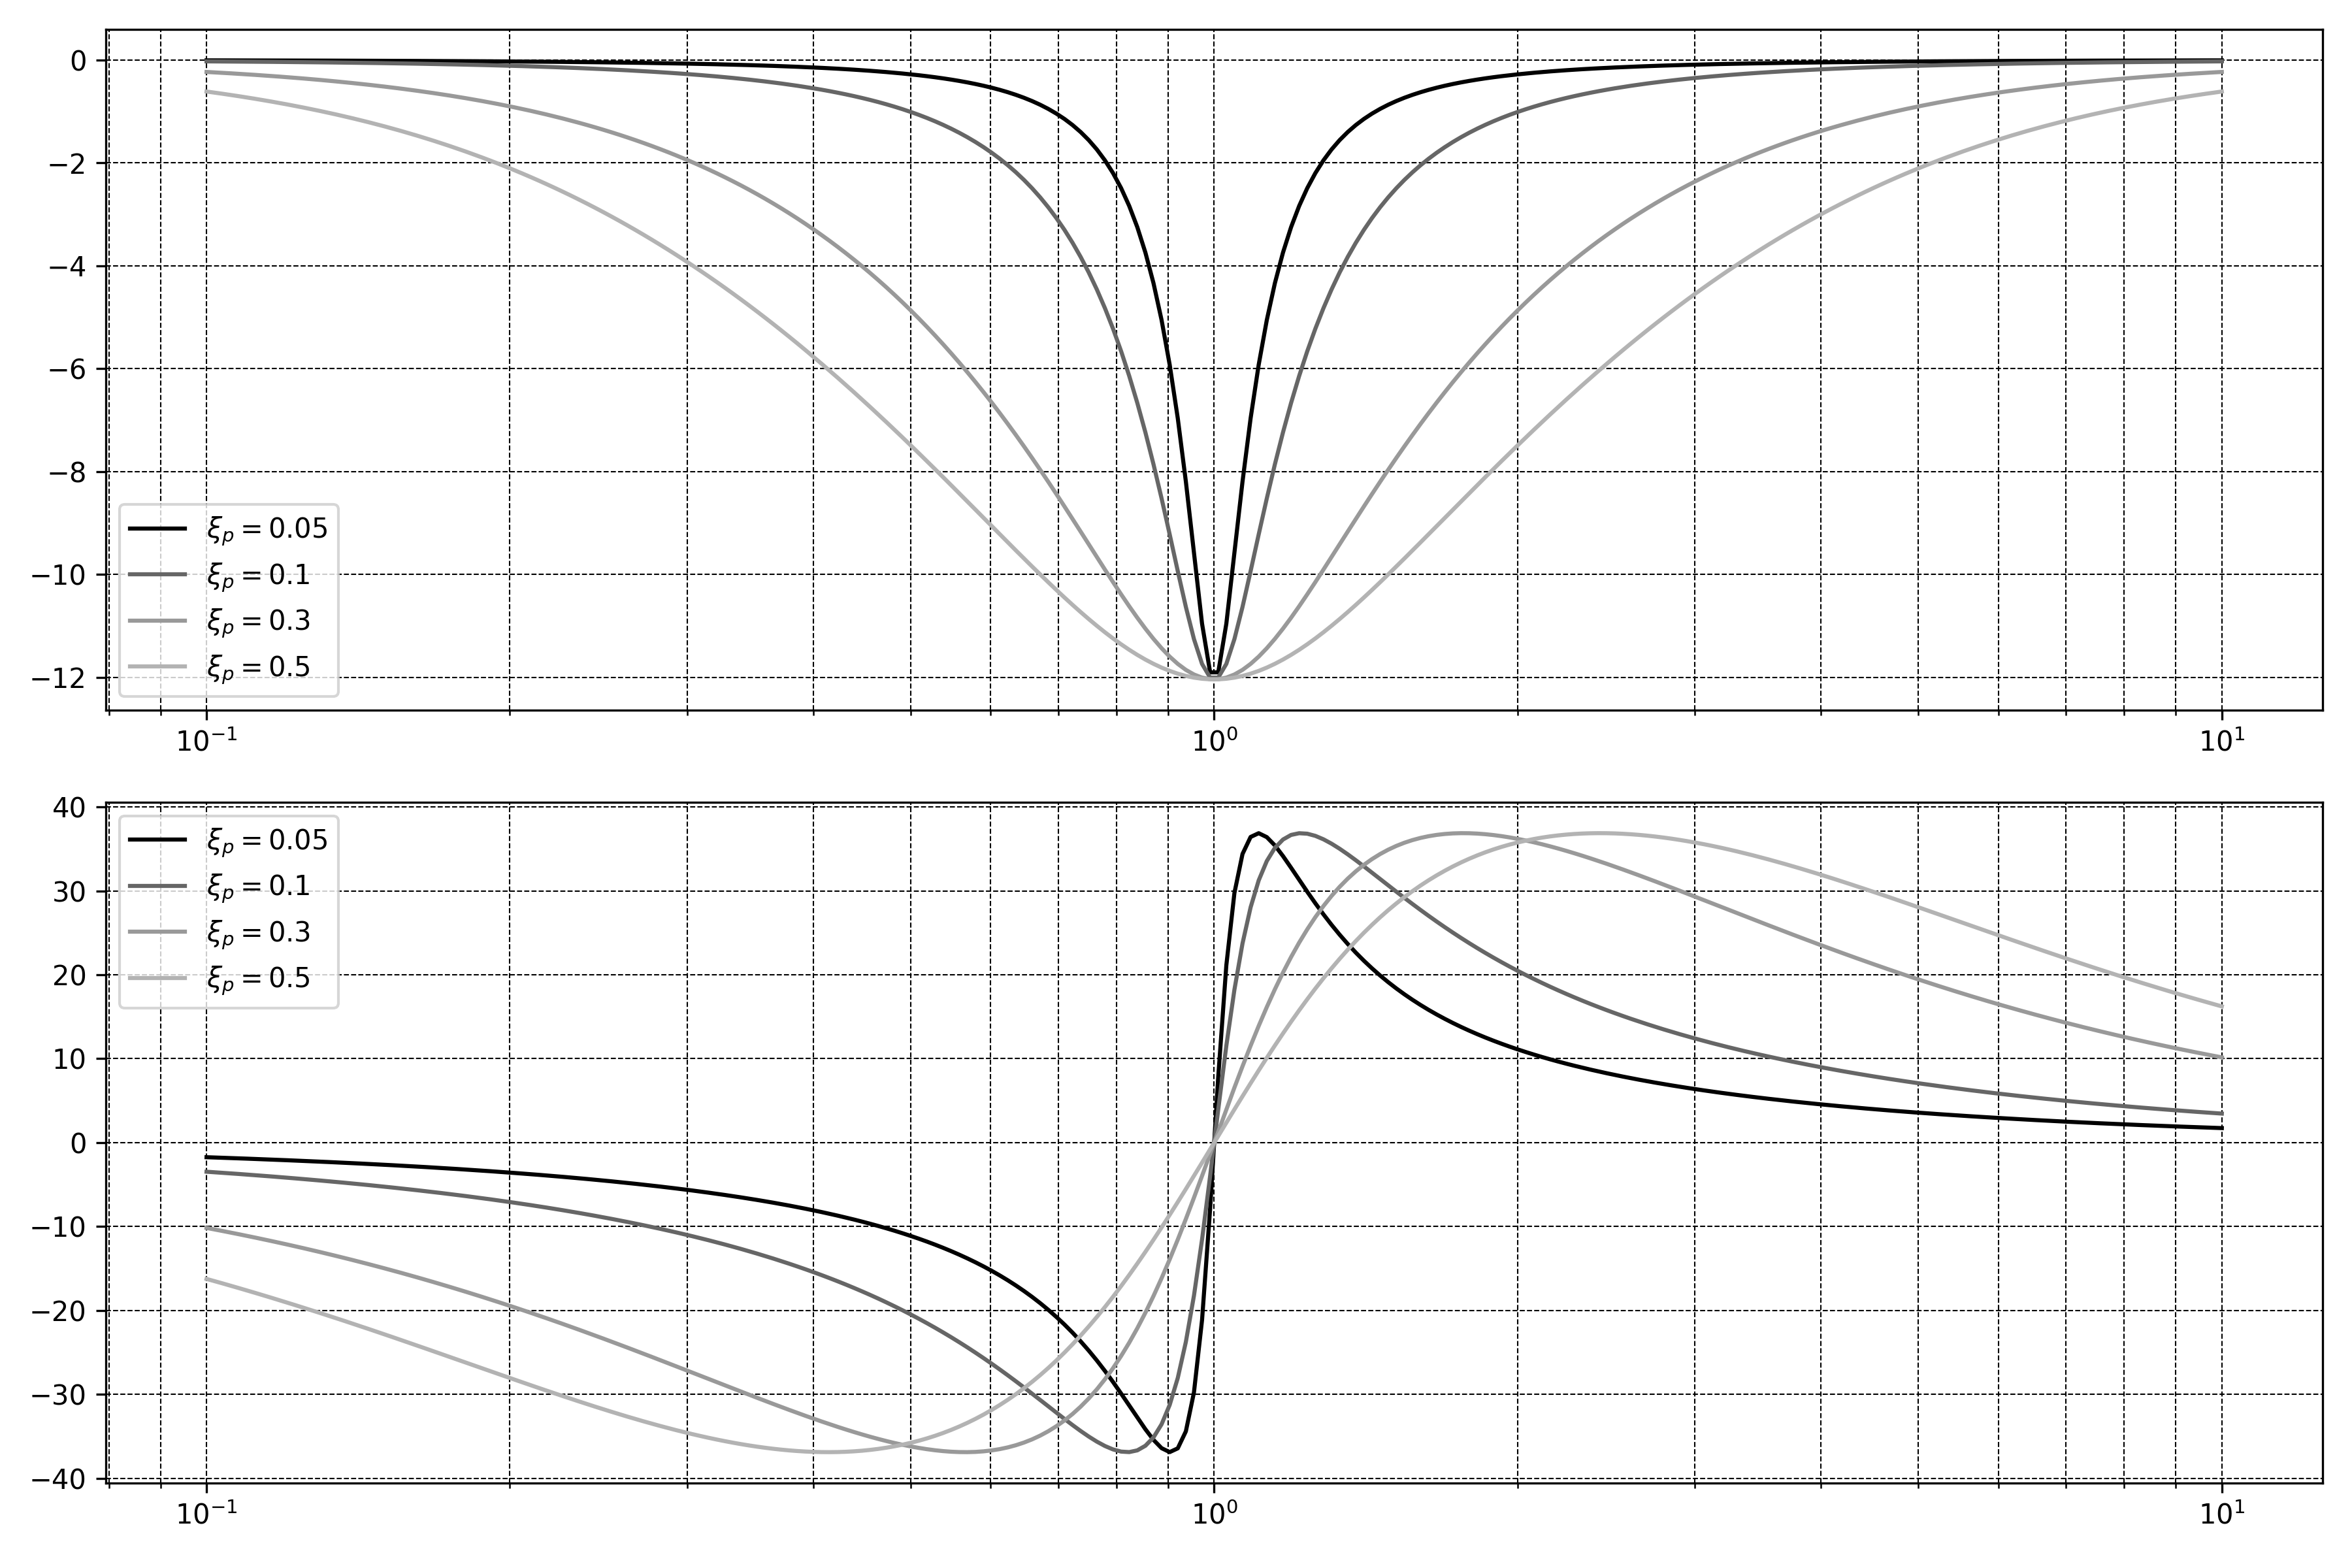
\includegraphics[width=0.3\textwidth]{Immagini/filtro_notch_xip_su_xid_costante.png}
    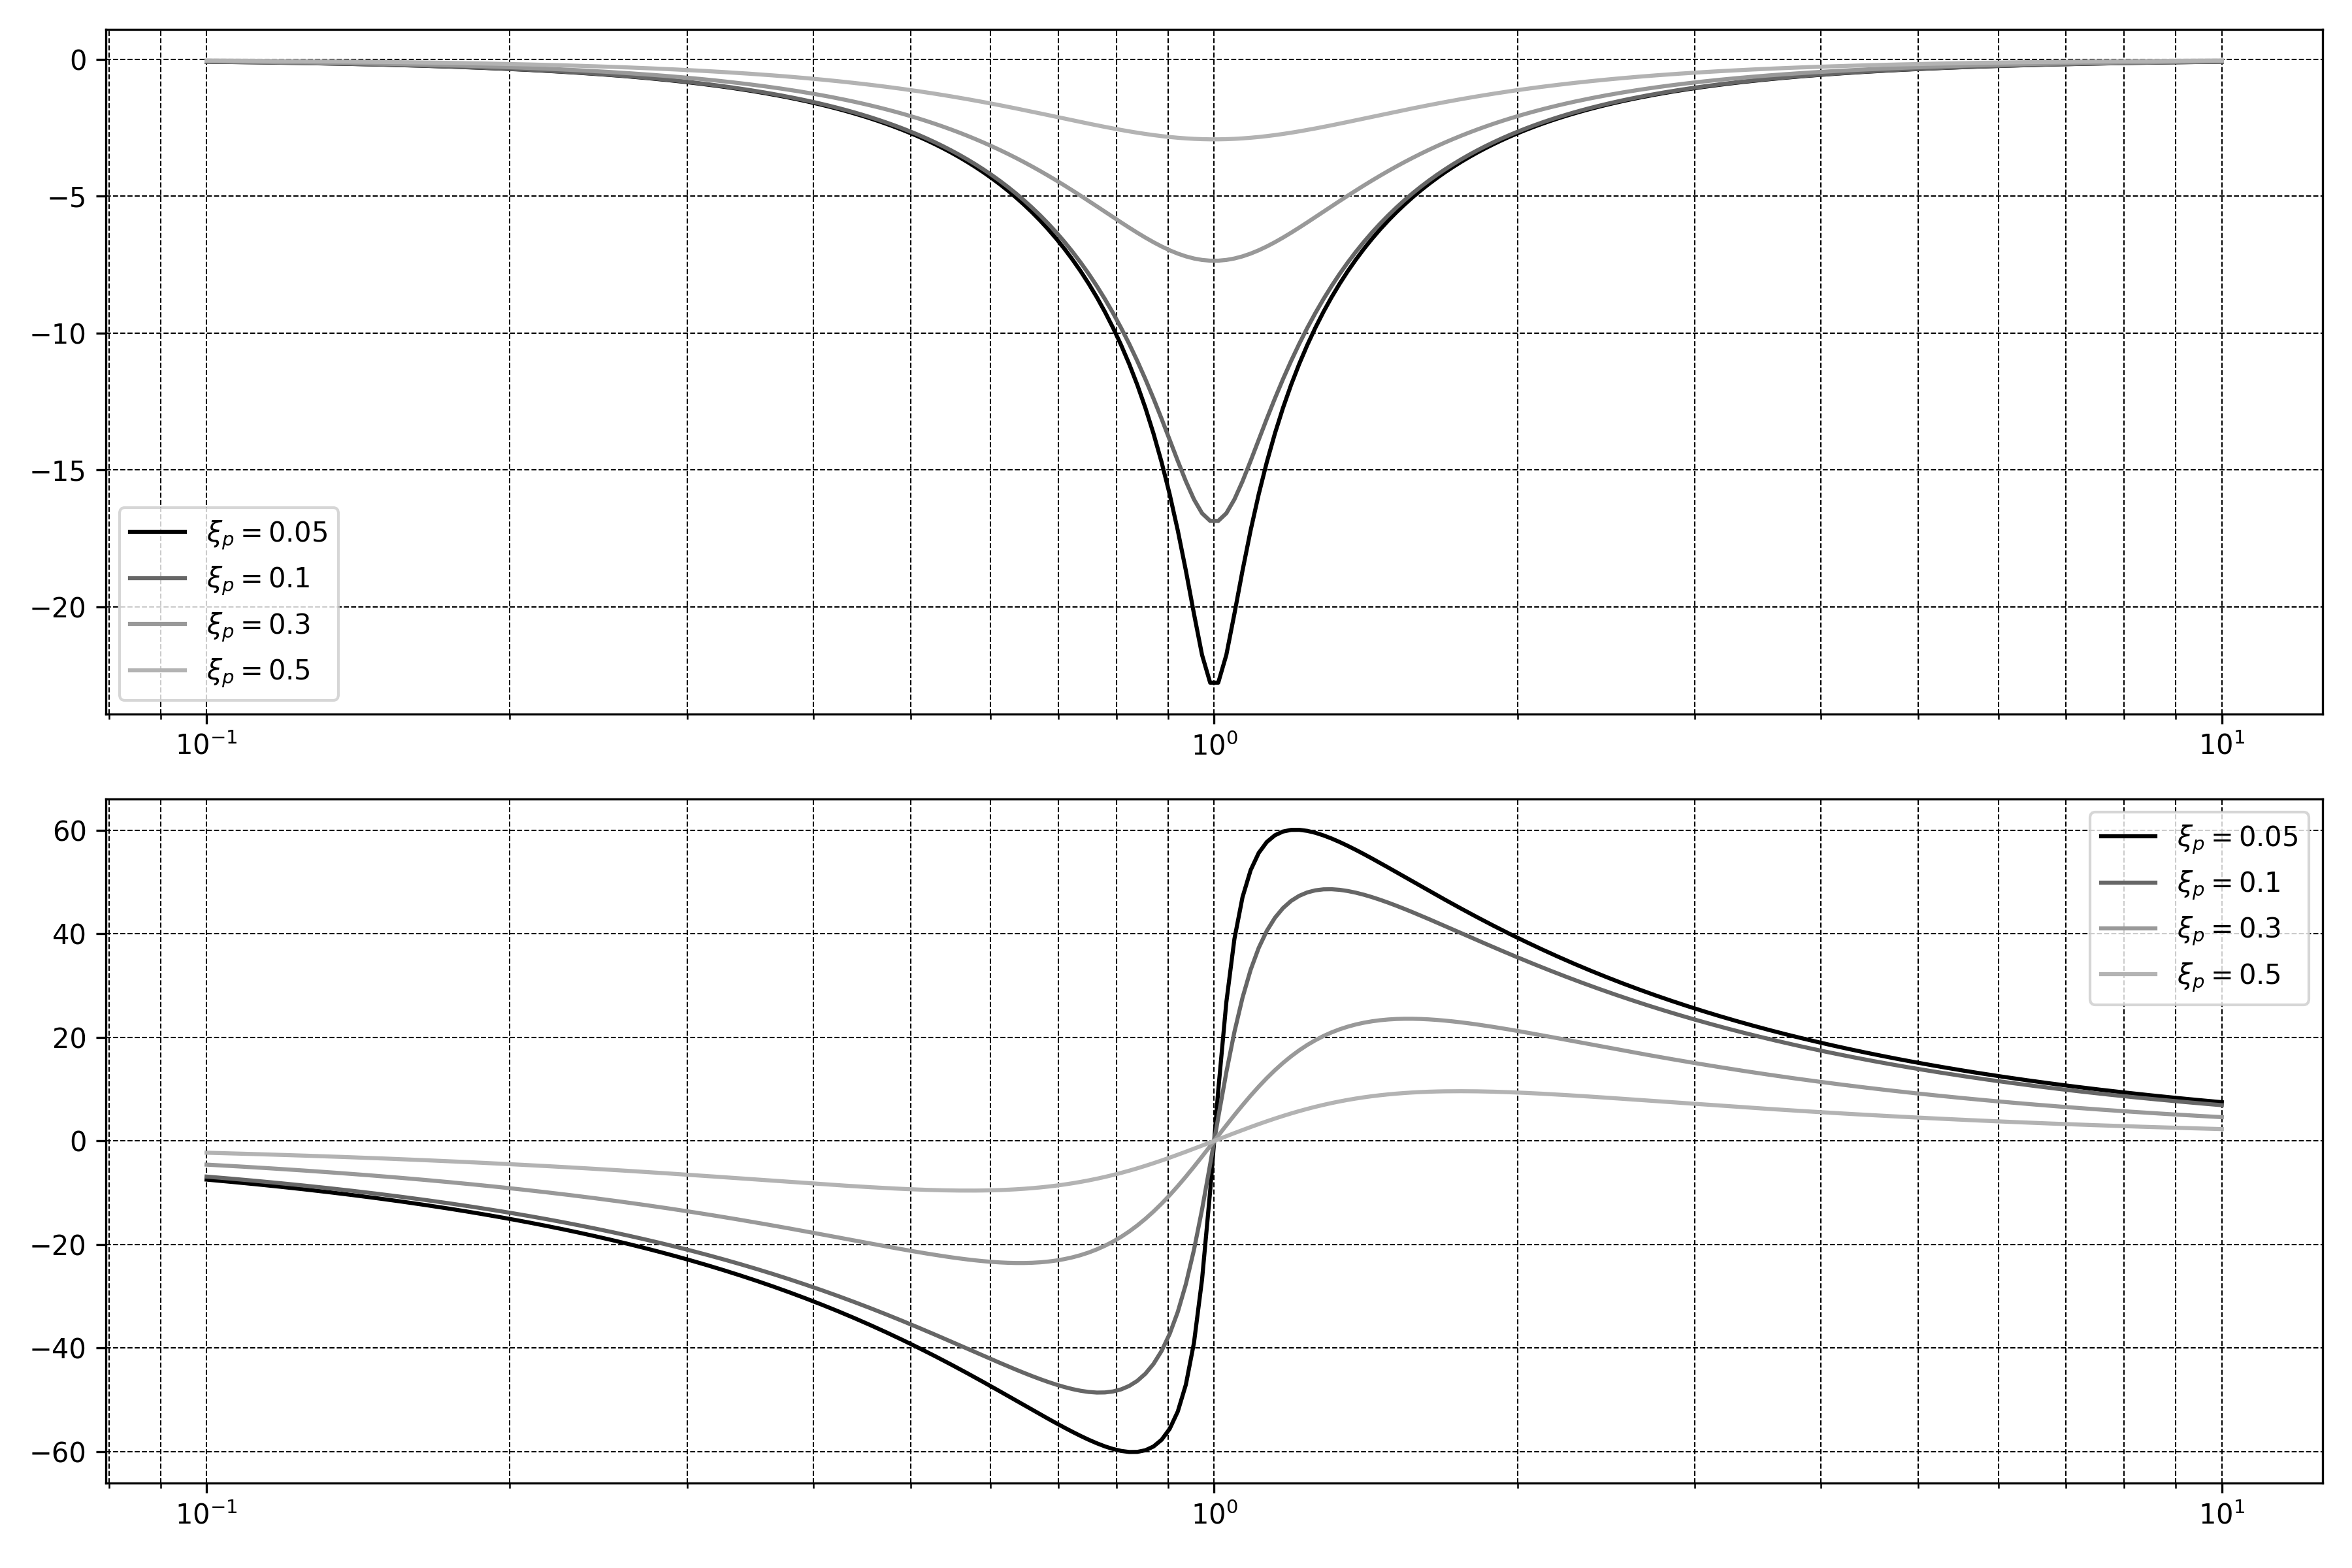
\includegraphics[width=0.3\textwidth]{Immagini/filtro_notch_xid_costante.png}
    \caption{Filtri notch: \(\xi_p\) costante sx, \(\frac{\xi_d}{\xi_p}\) costante centro, \(\xi_d\) costante dx}
\end{figure}

\sottoparagrafo{Biquadratici:}
L'idea dei filtri Biquadratici o BIQUAD è quella di implementare un filtro che sia l'inverso della mobilità di modo da cancellare poli e zeri \(F(s)=\frac{1}{G_{vm}(s)}\). Lato motore funziona molto bene, il controllo richiesto è quello per trasmissione rigida, tuttavia lato carico è presente il picco di risonanza legato alla presenza della trasmissibilità in catena aperta.
Richiede precisa sintonizzazione; aggiungere una risonanza nel filtro è rischioso se la sintonizzazione non è perfetta, perché potrebbe amplificare rumore bianco a quella frequenza.
Tuttavia potrebbe essere interessante se pensato come un "filtro notch a 4 parametri".

\sottoparagrafo{Filtri su Feedforward:}
Il filtro sul feedforward non modifica il margine di fase, nè la pulsazione di attraversamento, mentre rimuove le componenti armoniche di accelerazione prossime a \(\omega_p\) che potrebbero eccitare risonanza in caso di legge non dolce.
Resta importante la scelta della banda passante del filtro, perché il feedforward lavora soprattutto alle alte frequenze, perciò tagliare prima non permetterebbe un opportuno funzionamento.



\sezione{Anello di Posizione}
L'anello di posizione è l'anello più esterno del controllo, richiede perciò che l'anello di velocità sia stato ben sintonizzato, perché non ha modo di portare rimedio a problemi negli anelli più interni, anzi, semmai li peggiora.

\sottosezione{Controllo Co-Locato}

\import{Immagini}{anello_pos_colocato.tex}

Per una analisi semplificativa considero di trascurare: trasduttore di posizione, feedforward, anello di corrente e trasduttore di velocità.
Valuto i poli e gli zeri utilizzando il luogo delle radici, considerando che i poli di \(L_p\) sono i poli di \(W_v\) e il polo in \(s=0\) dovuto all'integrazione fisica; mentre gli zeri sono gli zeri di \(W_v\), che sono anche gli zeri di \(L_v\).

I poli di \(L_p\) sono i poli della della catena chiusa, tra i poli di \(L_v\) e \(W_v\) c'è il controllore, perciò occorre effettuare un opportuna scelta del guadagno di modo che i poli reali non diventino complessi coniugati.

\begin{figure}[h]
    \centering
    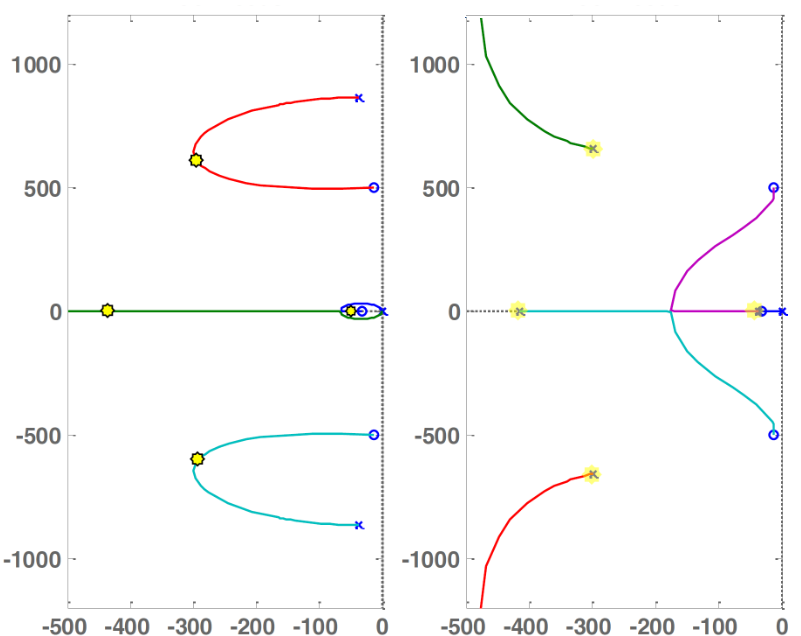
\includegraphics[width=0.4\textwidth]{Immagini/luogo_radici_colocato_vel_vs_pos.png}
    \caption{Luogo delle radici: velocità sx; posizione dx}
\end{figure}

\paragrafo{Analisi dei poli, scelta del guadagno:}
Il polo reale dell'integrale \(s=0\) per aumento del \(K_{pp}\) si muove verso lo zero reale, perciò, tanto più alto il guadagno, tanto più veloce diventa.
Tuttavia i poli reali "ereditati" dal controllo di velocità, per aumento di \(K_{pp}\) tenderebbero agli zeri dell'antirisonanza, quindi a diventare complessi coniugati, quindi a introdurre una bassa risonanza in bassa frequenza, motivo per cui è importante limitare il guadagno.
Per la scelta del guadagno si può utilizzare la formulazione empirica \(K_{pp}^{co} = \frac{\omega_{bv}}{4\xi_{des}^2}\), con \(\xi\in [1;1.5]\), mentre nel caso di risonanza in bassa o media frequenza è preferibile utilizzare \(\xi \simeq 1.4\), da cui \(K_{pp}^{co}\simeq \frac{\omega_{bv}}{8}\).

\begin{figure}[h]
    \centering
    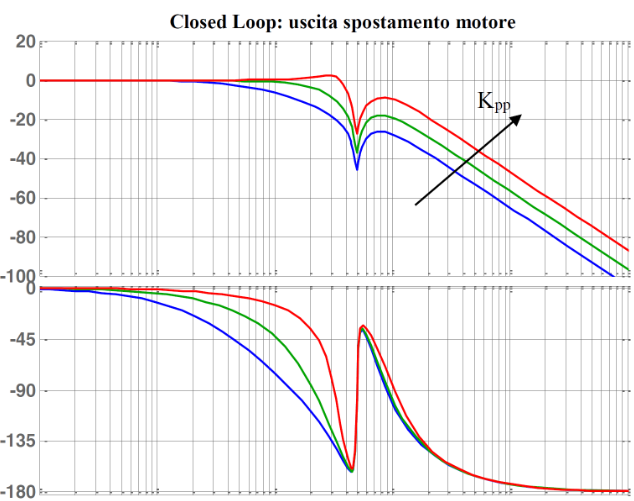
\includegraphics[width=0.35\textwidth]{Immagini/anello_chiuso_posizione_lato_motore.png}
    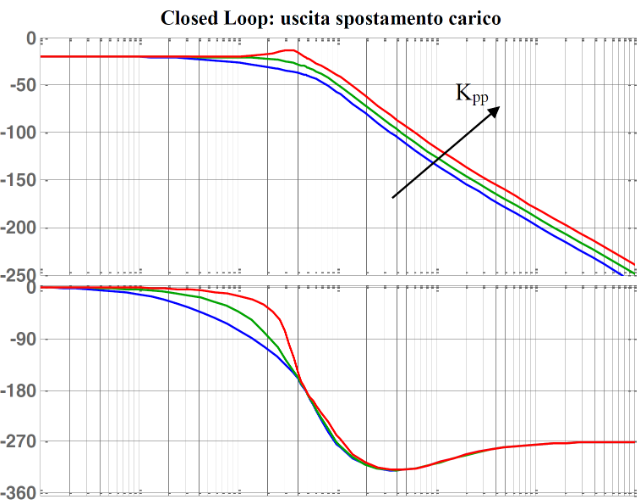
\includegraphics[width=0.35\textwidth]{Immagini/anello_chiuso_posizione_lato_carico.png}
    \caption{Anello chiuso posizione: lato motore sx; lato carico dx}
\end{figure}


\sottosezione{Controllo Non Co-Locato}

\import{Immagini}{anello_pos_non_colocato}

I poli di \(L_p\) sono i 4 poli di \(W_v\), 2 reali 2 complessi coniugati, il polo reale in \(s=0\) dovuto all'integrazione fisica e i 2 poli della trasmissibilità, che sono anche gli zeri complessi coniugati di \(W_v\).
Gli zeri di \(L_p\) sono i 3 zeri di \(W_v\), 2 complessi coniugati e uno reale, e lo zero della trasmissibilità.

%% inserire immagine rlocus

\paragrafo{Analisi controllo Non CoLocato, scelta guadagno:}
Per l'analisi del tipo di controllo si utilizza il luogo delle radici. Si vede come l'antirisonanza si cancelli con la risonanza in trasmissibilità; i due poli complessi coniugati tendono all'asse reale per \(K_{pp}\) elevati; polo reale in \(s=0\) tende a zero reale; infine, e parte più critica di questo controllo, i due poli reali tendono all'instabilità per \(K_{pp}\) elevati.
In modo simile al precedente, considero di dividere il controllo con un \(K_{pp}^{co}\) tra \(E_p^\text{carico}\), \(\Omega_{des}^\text{carico}\) e \(\frac{1}{\tau}\) tra \(\Omega_{des}^\text{carico}\), \(\Omega_{des}^\text{mot}\), risultando quindi in \(K_{pp}^{nc} = K_{pp}^{co} \frac{1}{\tau}\).
Attenzione che questo non significa che il guadagno è alzato dal riduttore, perché quel \(\frac{1}{\tau}\) va a elidersi con il \(\tau\) della trasmissibilità.

%% inserire immagine concetto del guadagno

\sottosottosezione{CoLocato vs Non CoLocato}
Il controllo di tipo CoLocato è incondizionatamente stabile\footnote{Teoricamente, in pratica ci sono delle dinamiche finora ignorate che renderanno instabile il controllo per \(K_{pp}\) eccessivamente elevati.}; il controllo Non CoLocato invece tende all'instabilità per \(K_{pp}\) elevati.
Per \(K_{pp}\) bassi i due hanno comportamenti molto simili, perciò in potenziali applicazioni si può usare uno o l'altro in base alle condizioni operative.

\paragrafo{Condizione di disturbo al carico:}
Il controllo di tipo Non CoLocato è da utilizzare nel caso di forze di disturbo al carico rilevanti. 

Partendo dall'equazione della dinamica lato carico \(J_c \AccAng_c = -k(\theta_c - \theta_m \tau_R) - D(\VelAng_c - \VelAng_m\tau_R) - C_c - f_c\VelAng_c\), considerando condizioni statiche, rapporto di trasmissione unitario, si ottiene \(C_c = k(\theta_c - \theta_m)\).
Applicando un gradino di coppia di carico, si ottiene che a regime vale \(\theta_c - \theta_m = \frac{C_c}{k}\), ossia motore e carico non avranno la stessa posizione finale.

Con controllo di tipo colocato questa differenza non viene percepita, perché il motore verrà correttamente portato al suo valore finale, mentre il carico sarà ad una posizione non nota e scorretta.
Con il controllo non colocato invece, misurando la posizione del carico, questa sarà corretta, e il motore andrà a compensare la differenza.

La scelta tra i due quindi è legata a valutazione del tipo \(\frac{C_c^\text{attesa}}{K^\text{stimata}} < \text{precisione desiderata lato carico}\), se viene rispettata questa disuguaglianza si può utilizzare un controllo colocato, altrimenti occorre usare uno non colocato.

\paragrafo{Quando NON usare controllo non colocato:}
Il controllo non colocato è legato a margine di fase minore e necessità di opportune scelte, dimensionamento, implementazione\footnote{L'encoder richiede installazione accurata, deve essere installato utilizzando un elemento rigido, altrimenti si potrebbe aggiungere risonanza e antirisonanza indesiderata nella misura.} di trasduttori lato carico, perciò meno di forze di disturbo al carico elevate, non è conveniente rispetto un CoLocato.

Il controllo non colocato va evitato in caso di gioco elevato, perché avere gioco significa avere una zona di incertezza in cui non si può sapere esattamente dov'è il carico; però il controllo tenderebbe ugualmente alla posizione desiderata, ma se l'incertezza è tale da portare il carico fuori dalla zona di incertezza, questo tenterebbe di riportarlo in posizione desiderata, ma con alto errore, quindi alta compensazione, quindi tenderebbe a uscire dalla zona di incertezza lato opposto, portando a oscillazione di posizione del carico oltre la zona di incertezza. Fenomeno peggiorato per \(K_{pp}\) elevato.
Risolvere questa problematica richiede utilizzo di guadagni variabili con la velocità e in particolare ulteriormente ridotti per basse velocità, quindi prossimi a regime.